\documentclass[11pt,a4paper]{article}
\usepackage[latin1]{inputenc}
\usepackage{amsmath}
\usepackage{amsfonts}
\usepackage[super,sort&compress,comma]{natbib}
\usepackage{amssymb}
\usepackage{graphicx}
\usepackage{hyperref}
\usepackage{siunitx}
\author{Andrew R. McCluskey,\textit{$^{ab}$}$^{\ddag}$ Adrian Sanchez-Fernandez,\textit{$^{ac}$}$^{\ddag\P}$ \\
Karen J. Edler,\textit{$^{a}$}$^{\ast}$ Stephen C. Parker,\textit{$^{a}$} Andrew J. Jackson,\textit{$^{cd}$} \\
Richard A. Campbell,\textit{$^{ef}$} and Thomas Arnold\textit{$^{abcg}$}$^{\ast}$ \\
 \\
\textit{$^{a}$~Department of Chemistry, University of Bath, Claverton} \\
\textit{Down, Bath, BA2 7AY, UK.} \\
\textit{$^{b}$~Diamond Light Source, Harwell Campus, Didcot, OX11 0DE,} \\
\textit{UK.} \\
\textit{$^{c}$~European Spallation Source, SE-211 00 Lund, Sweden.} \\
\textit{$^{d}$~Department of Physical Chemistry, Lund University,} \\
\textit{SE-211 00 Lund, Sweden.} \\
\textit{$^{e}$~Institut Laue-Langevin, 71 avenue des Martyrs, 38000,} \\
\textit{Grenoble, France.} \\
\textit{$^{f}$~Division of Pharmacy and Optometry, University of} \\
\textit{Manchester, Manchester, M13 9PT, UK.} \\
\textit{$^{g}$~ISIS Neutron and Muon Source, Science and Technology} \\
\textit{Facilities Council, Rutherford Appleton Laboratory, Harwell} \\
\textit{Oxford, Didcot OX11 0QX, UK.} \\
\textit{$^{\P}$~Present address: Department of Food Technology, Lund} \\
\textit{University, SE-211 00 Lund, Sweden}}
\title{ESI for ``Bayesian determination of the effect of a deep eutectic solvent on the structure of lipid monolayers''}
\date{}
\begin{document}

\maketitle
\section{Grazing incident X-ray diffraction (GIXD)}
GIXD was measured for DPPC and DMPC at \SI{30}{\milli\newton\per\meter} at \SI{22}{\celsius} (and \SI{7}{\celsius} for DMPC), and are shown in Figures \ref{fig:dppcgixd}-\ref{fig:dmpcgixd7}. All figures contain an artifact from the X-ray beam interacting with the Teflon of the Langmuir trough. However, in figures \ref{fig:dppcgixd} and \ref{fig:dmpcgixd7} it is possible to identify a (2, 0) diffraction peak that indicates the presence of a similar structure to that found under the same conditions in water.\cite{Watkins2009} Based on this information we believe that, similar to water, the phase of the lipid tails is likely to be in the liquid phase at all surface pressures measured.
\begin{figure}[h]
	\centering
	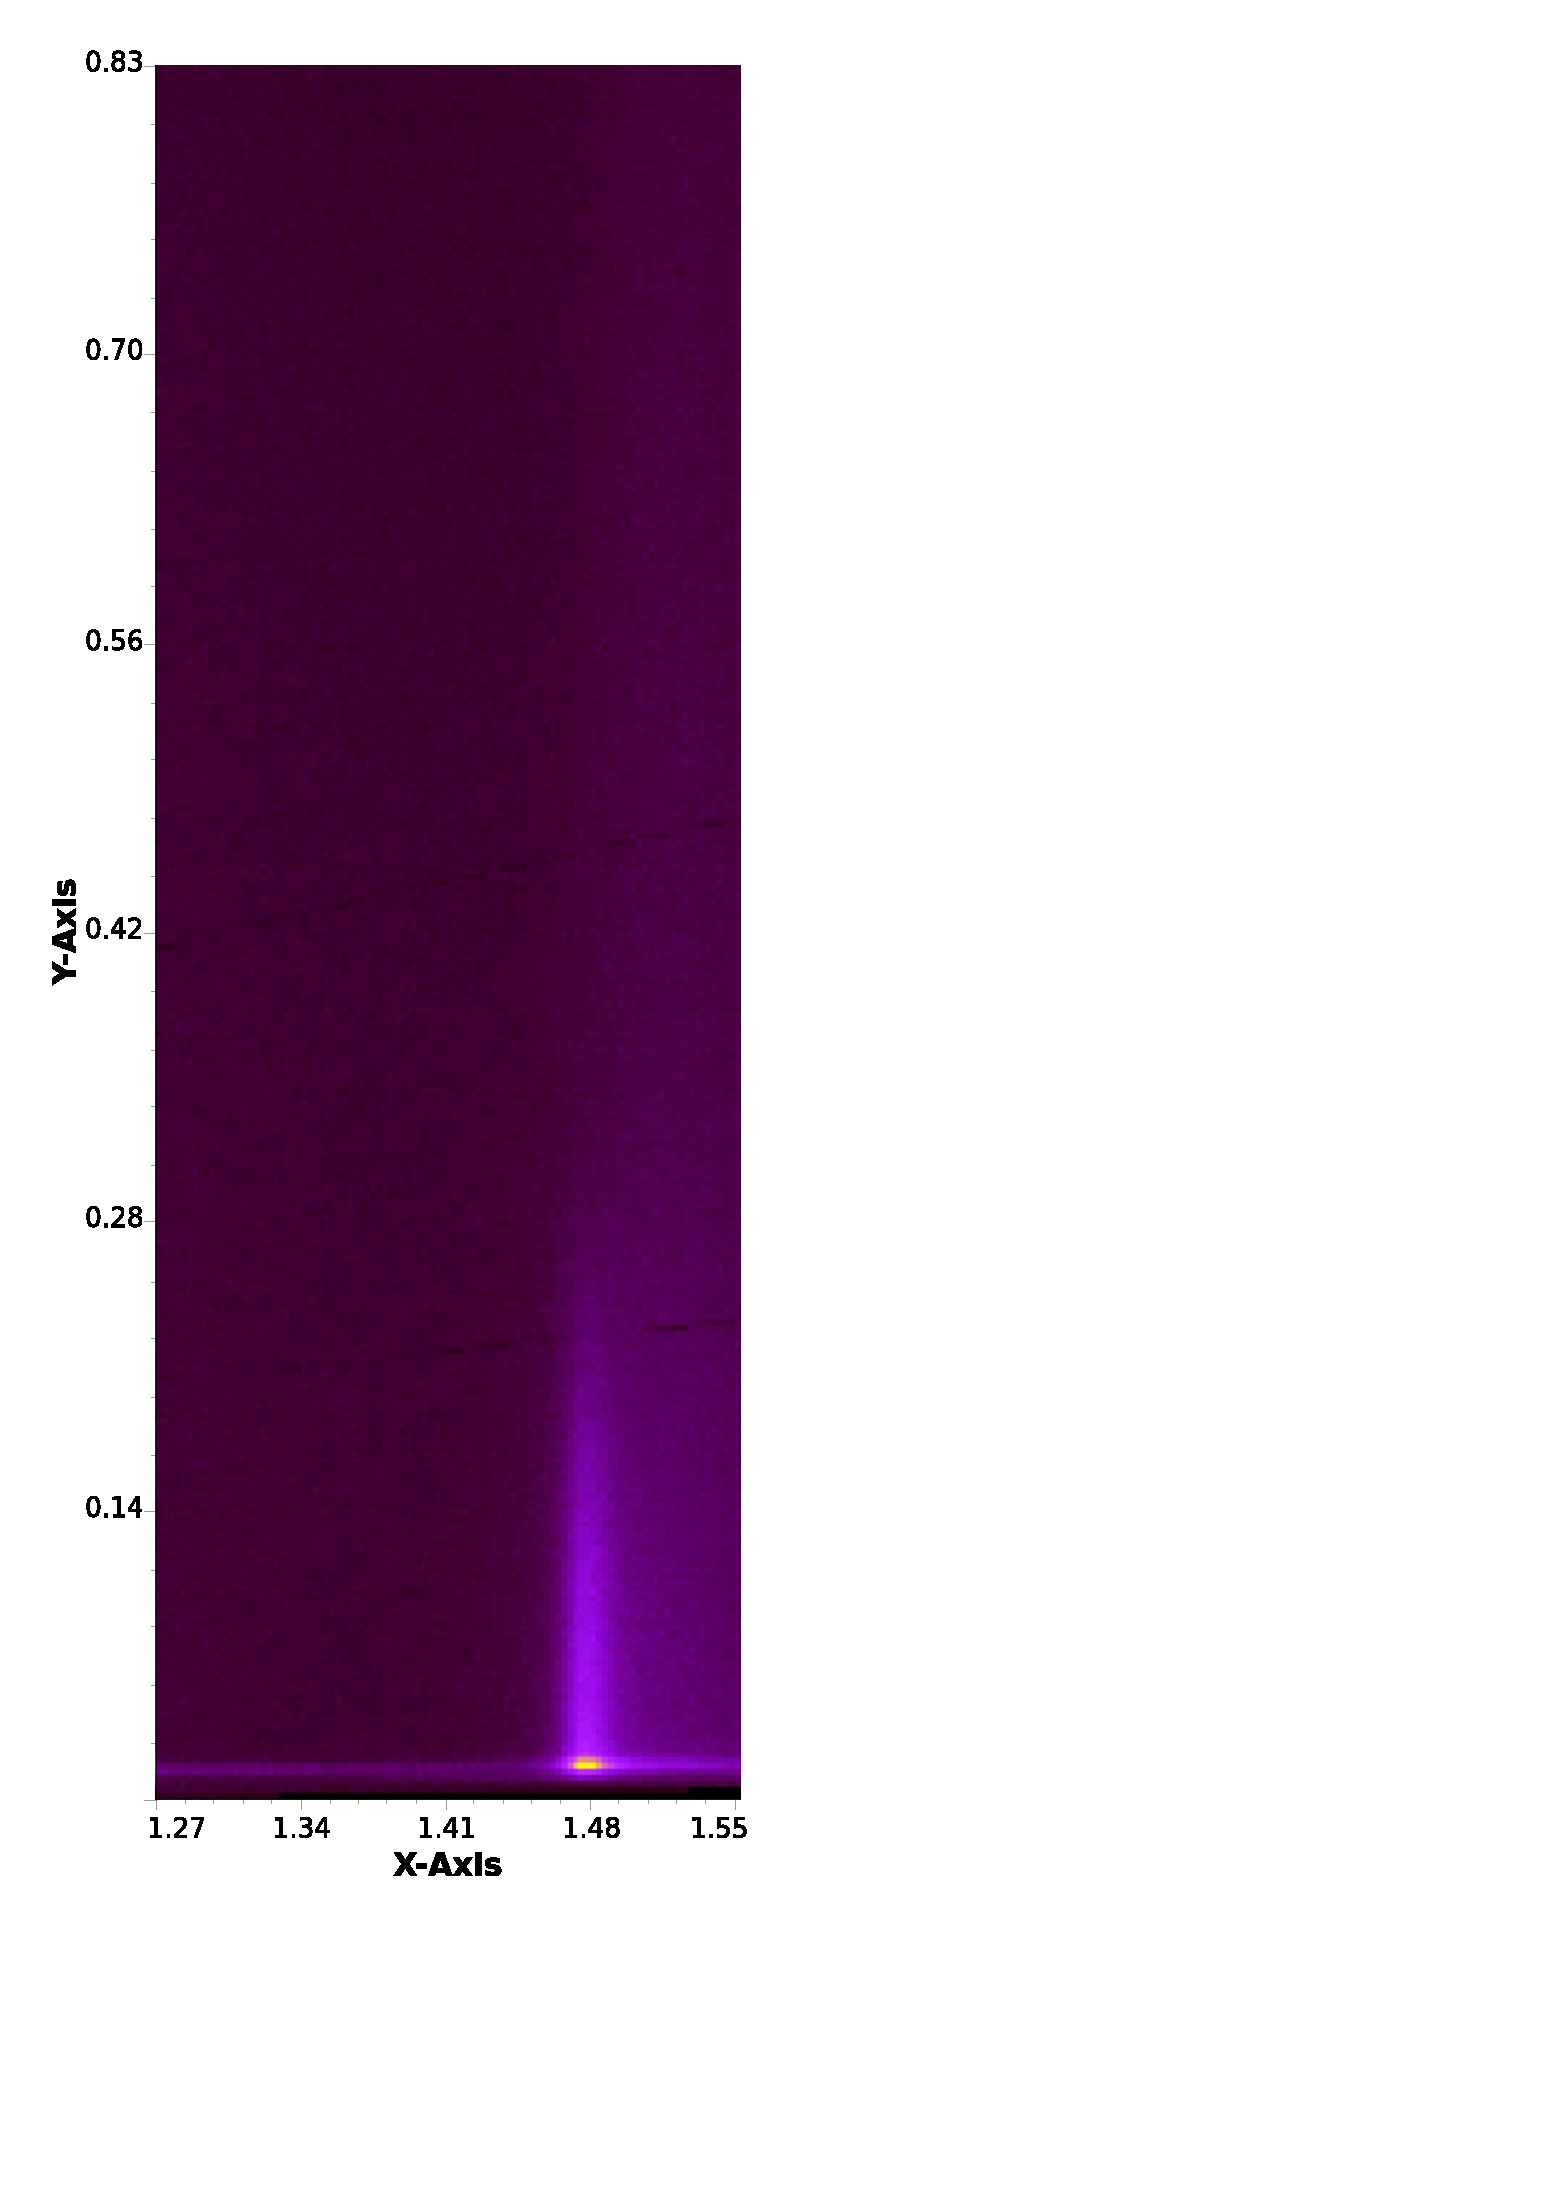
\includegraphics[width=0.50\textwidth]{figures/206041}
	\caption{The GIXD pattern for DPPC at \SI{30}{\milli\newton\per\meter} at \SI{22}{\celsius}, the axes at in units of \si{\per\angstrom}. Source: Datasets, figure files and running/plotting scripts are available under CC-BY.\cite{mccluskey_2018}}
	\label{fig:dppcgixd}
\end{figure}
\begin{figure}[h]
	\centering
	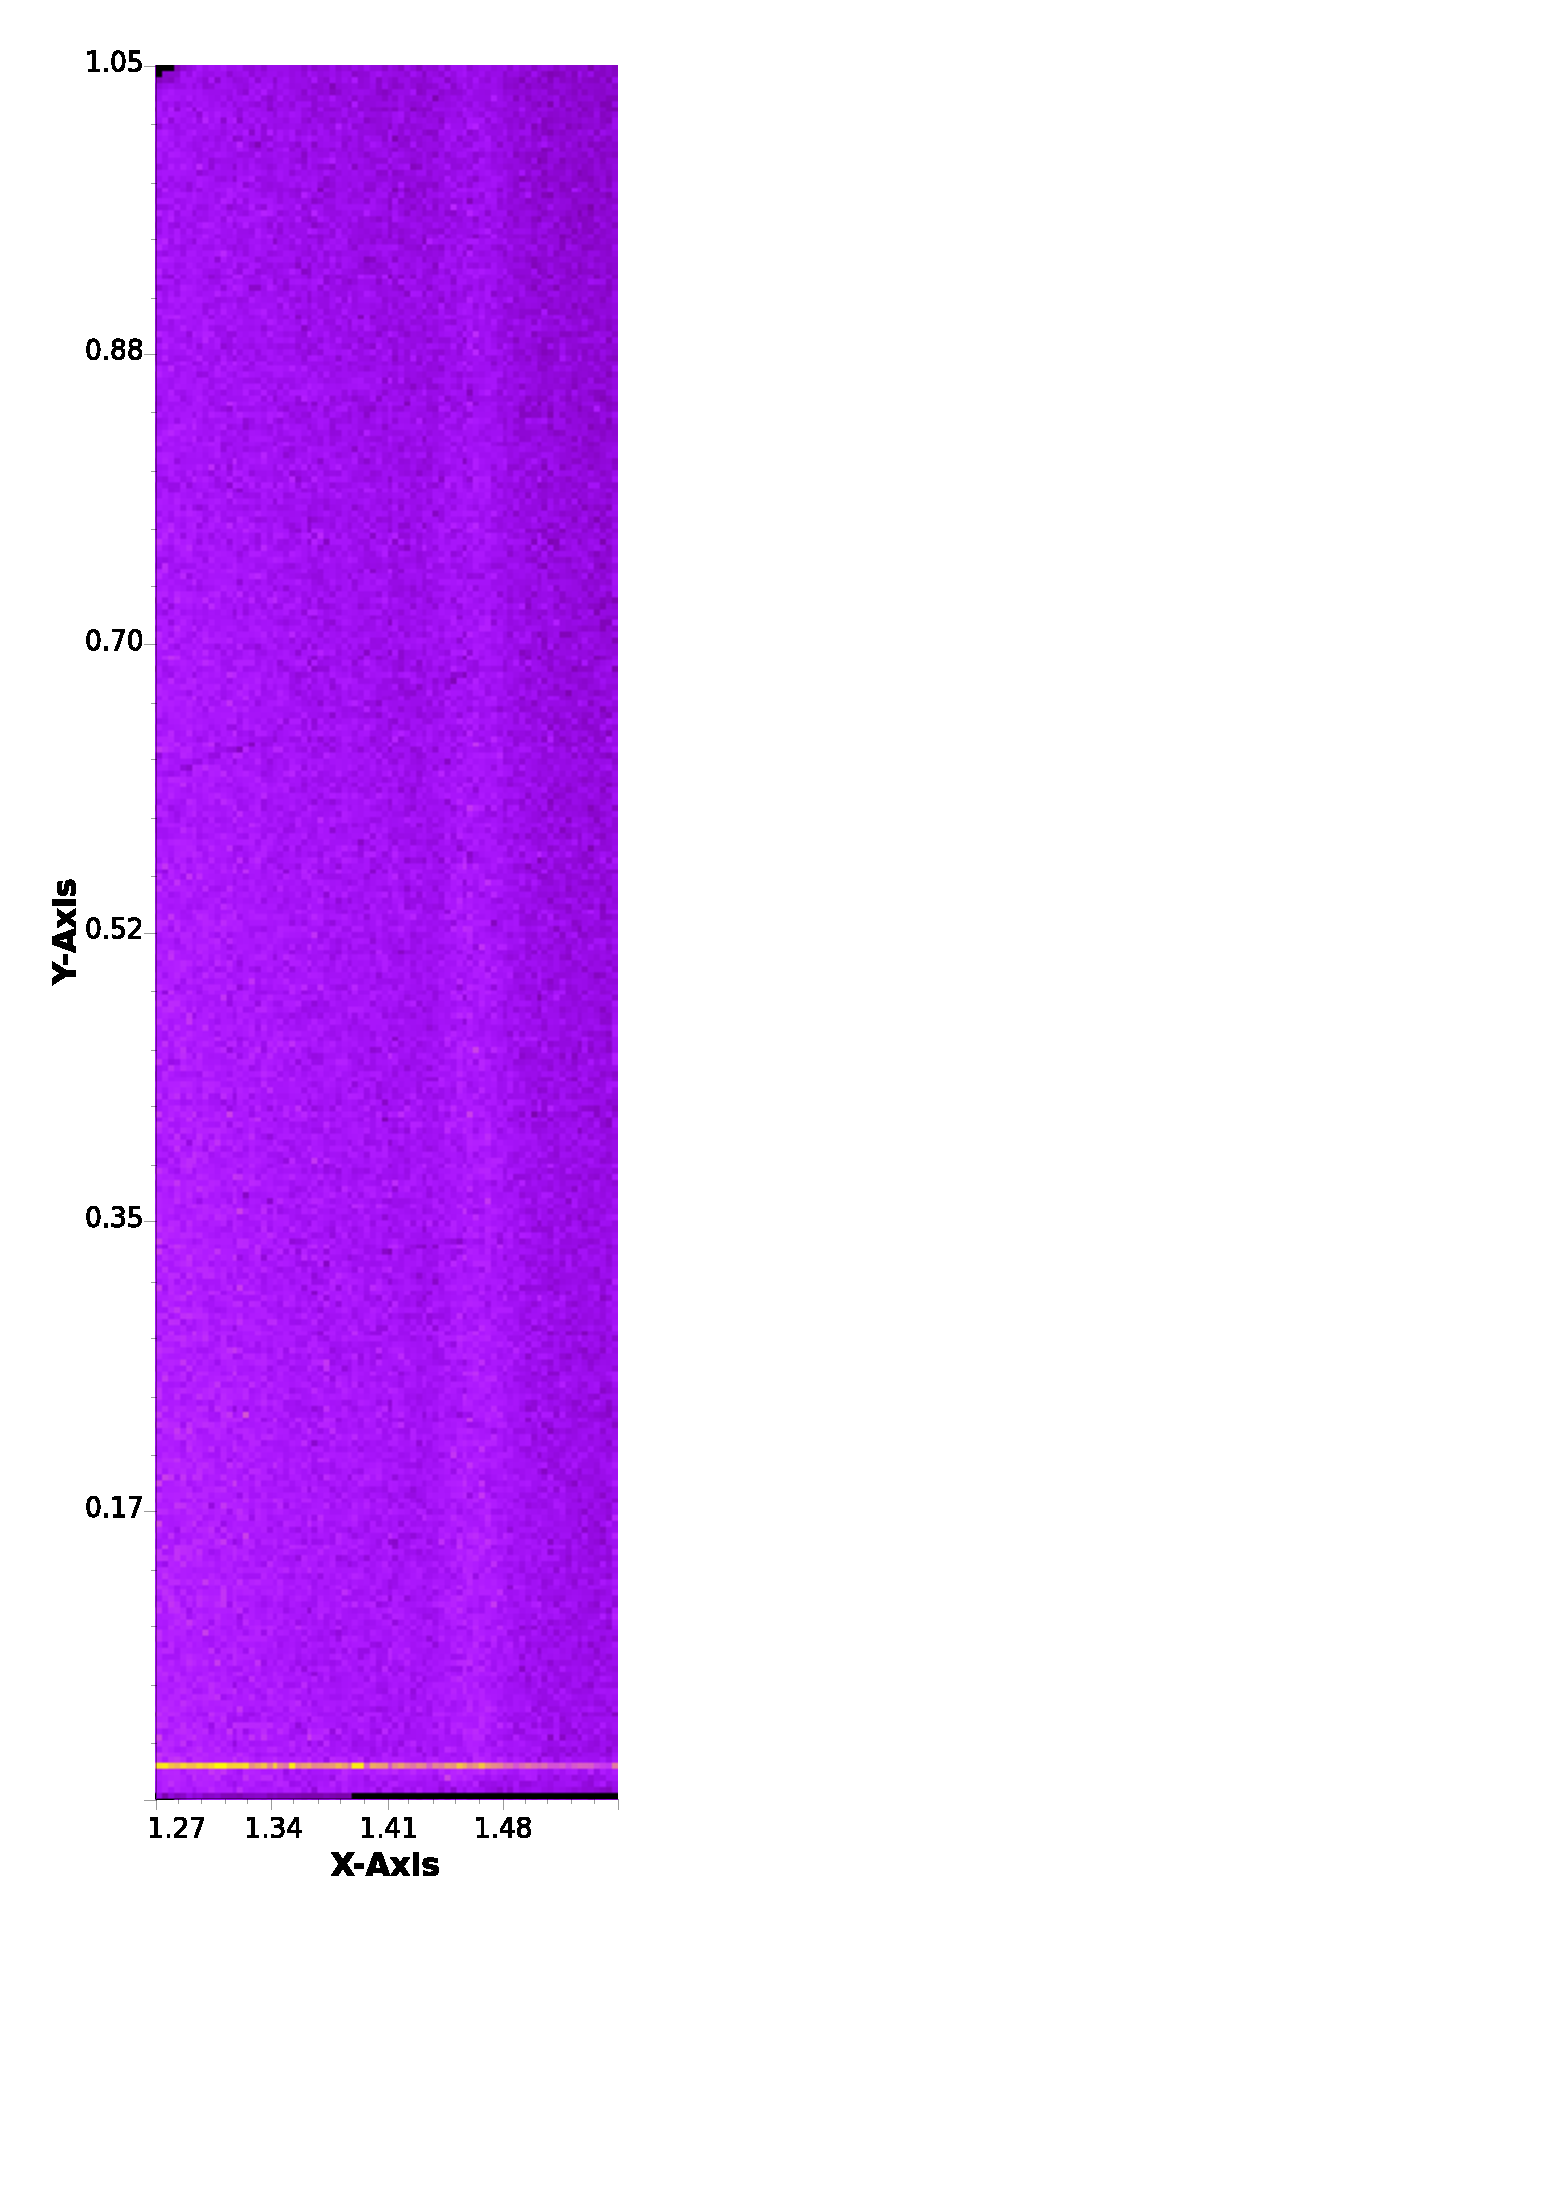
\includegraphics[width=0.50\textwidth]{figures/206151}
	\caption{The GIXD pattern for DMPC at \SI{30}{\milli\newton\per\meter} at \SI{22}{\celsius}, the axes at in units of \si{\per\angstrom}. Source: Datasets, figure files and running/plotting scripts are available under CC-BY.\cite{mccluskey_2018}}
	\label{fig:dmpcgixd}
\end{figure}
\begin{figure}[h]
	\centering
	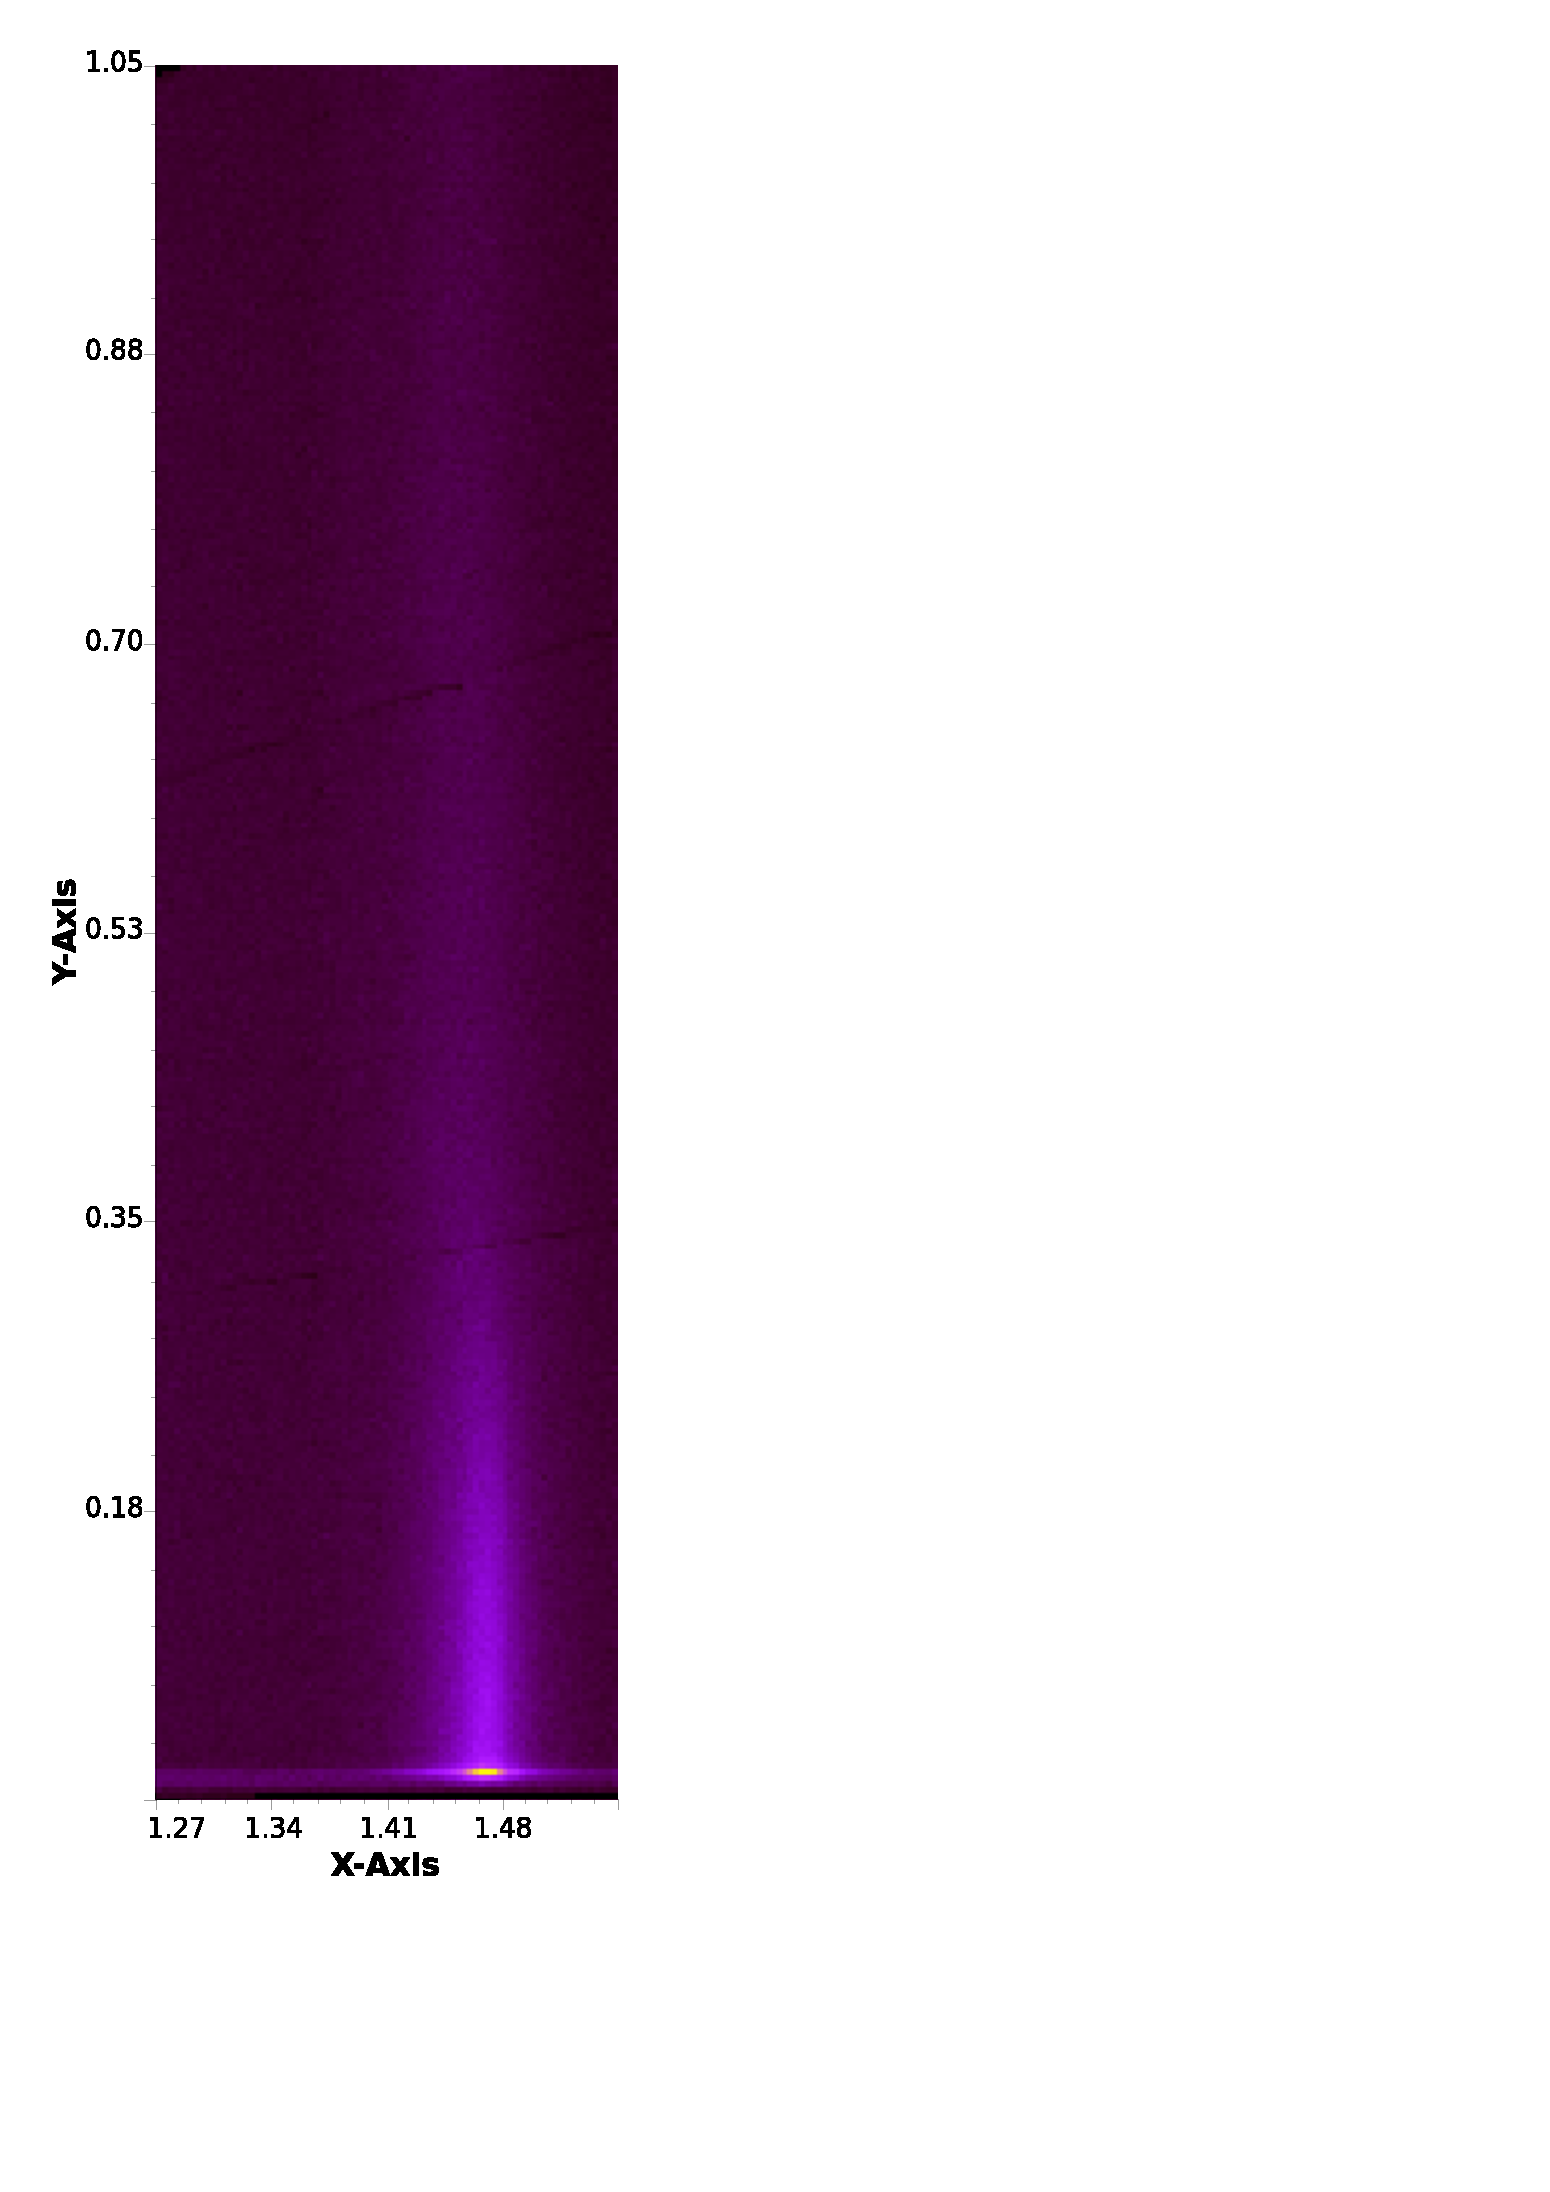
\includegraphics[width=0.50\textwidth]{figures/206161}
	\caption{The GIXD pattern for DMPC at \SI{30}{\milli\newton\per\meter} at \SI{7}{\celsius}, the axes at in units of \si{\per\angstrom}. Source: Datasets, figure files and running/plotting scripts are available under CC-BY.\cite{mccluskey_2018}}
	\label{fig:dmpcgixd7}
\end{figure}

\section{XRR parameters at each surface pressure}

%
\begin{table}
	\caption{\ The best-fit values, and associated 95 \% confidence intervals for the varying parameters in the XRR models, at the second highest surface pressure (SP) measured. The values of $d_t$ were found from the values of $\theta_t$ using Eqn. \ref{equ:tl} and the values for $\phi_h$ were obtained from the use of Eqn. \ref{equ:phih}}
	\label{tab:liptab1}
	\begin{tabular*}{0.48\textwidth}{@{\extracolsep{\fill}}lllll}
		\hline
		Lipid & DLPC & DMPC & DPPC & DMPG \\
    SP/mNm$^{-1}$ & 30 & 30 & 25 & 25 \\
		\hline
		$\theta_t$/$^\circ$ & \input{../output/dlpc/angle30.txt} & \input{../output/dmpc/angle30.txt} & \input{../output/dppc/angle25.txt} & \input{../output/dmpg/angle25.txt} \\
		$\sigma_{t,h,s}$/\AA & \input{../output/dlpc/rough30.txt} & \input{../output/dmpc/rough30.txt} & \input{../output/dppc/rough25.txt} & \input{../output/dmpg/rough25.txt} \\
    \hline
    $V_t$/\AA$^3$ & \input{../output/dlpc/vt.txt} & \input{../output/dmpc/vt.txt} & \input{../output/dppc/vt.txt} & \input{../output/dmpg/vt.txt} \\
		$V_h$/\AA$^3$ & \input{../output/dlpc/vh.txt} & \input{../output/dmpc/vh.txt} & \input{../output/dppc/vh.txt} & \input{../output/dmpg/vh.txt} \\
		$d_h$/\AA & \input{../output/dlpc/head.txt} & \input{../output/dmpc/head.txt} & \input{../output/dppc/head.txt} & \input{../output/dmpg/head.txt} \\
    \hline
    $\phi_h$/$\times10^{-2}$ & \input{../output/dlpc/solh30.txt} & \input{../output/dmpc/solh30.txt} & \input{../output/dppc/solh25.txt} & \input{../output/dmpg/solh25.txt} \\
		$d_t$/\AA & \input{../output/dlpc/tail30.txt} & \input{../output/dmpc/tail30.txt} & \input{../output/dppc/tail25.txt} & \input{../output/dmpg/tail25.txt} \\
		\hline
	\end{tabular*}
\end{table}
%
%
\begin{table}
	\caption{\ The best-fit values, and associated 95 \% confidence intervals for the varying parameters in the XRR models, at the second lowest surface pressure (SP) measured. The values of $d_t$ were found from the values of $\theta_t$ using Eqn. \ref{equ:tl} and the values for $\phi_h$ were obtained from the use of Eqn. \ref{equ:phih}}
	\label{tab:liptab2}
	\begin{tabular*}{0.48\textwidth}{@{\extracolsep{\fill}}lllll}
		\hline
		Lipid & DLPC & DMPC & DPPC & DMPG \\
    SP/mNm$^{-1}$ & 25 & 25 & 20 & 20 \\
		\hline
		$\theta_t$/$^\circ$ & \input{../output/dlpc/angle25.txt} & \input{../output/dmpc/angle25.txt} & \input{../output/dppc/angle20.txt} & \input{../output/dmpg/angle20.txt} \\
		$\sigma_{t,h,s}$/\AA & \input{../output/dlpc/rough25.txt} & \input{../output/dmpc/rough25.txt} & \input{../output/dppc/rough20.txt} & \input{../output/dmpg/rough20.txt} \\
    \hline
    $V_t$/\AA$^3$ & \input{../output/dlpc/vt.txt} & \input{../output/dmpc/vt.txt} & \input{../output/dppc/vt.txt} & \input{../output/dmpg/vt.txt} \\
		$V_h$/\AA$^3$ & \input{../output/dlpc/vh.txt} & \input{../output/dmpc/vh.txt} & \input{../output/dppc/vh.txt} & \input{../output/dmpg/vh.txt} \\
		$d_h$/\AA & \input{../output/dlpc/head.txt} & \input{../output/dmpc/head.txt} & \input{../output/dppc/head.txt} & \input{../output/dmpg/head.txt} \\
    \hline
    $\phi_h$/$\times10^{-2}$ & \input{../output/dlpc/solh25.txt} & \input{../output/dmpc/solh25.txt} & \input{../output/dppc/solh20.txt} & \input{../output/dmpg/solh20.txt} \\
		$d_t$/\AA & \input{../output/dlpc/tail25.txt} & \input{../output/dmpc/tail25.txt} & \input{../output/dppc/tail20.txt} & \input{../output/dmpg/tail20.txt} \\
		\hline
	\end{tabular*}
\end{table}
%
%
\begin{table}
	\caption{\ The best-fit values, and associated 95 \% confidence intervals for the varying parameters in the XRR models, at the lowest surface pressure (SP) measured. The values of $d_t$ were found from the values of $\theta_t$ using Eqn. \ref{equ:tl} and the values for $\phi_h$ were obtained from the use of Eqn. \ref{equ:phih}}
	\label{tab:liptab3}
	\begin{tabular*}{0.48\textwidth}{@{\extracolsep{\fill}}lllll}
		\hline
		Lipid & DLPC & DMPC & DPPC & DMPG \\
    SP/mNm$^{-1}$ & 20 & 20 & 15 & 15 \\
		\hline
		$\theta_t$/$^\circ$ & \input{../output/dlpc/angle20.txt} & \input{../output/dmpc/angle20.txt} & \input{../output/dppc/angle15.txt} & \input{../output/dmpg/angle15.txt} \\
		$\sigma_{t,h,s}$/\AA & \input{../output/dlpc/rough20.txt} & \input{../output/dmpc/rough20.txt} & \input{../output/dppc/rough15.txt} & \input{../output/dmpg/rough15.txt} \\
    \hline
    $V_t$/\AA$^3$ & \input{../output/dlpc/vt.txt} & \input{../output/dmpc/vt.txt} & \input{../output/dppc/vt.txt} & \input{../output/dmpg/vt.txt} \\
		$V_h$/\AA$^3$ & \input{../output/dlpc/vh.txt} & \input{../output/dmpc/vh.txt} & \input{../output/dppc/vh.txt} & \input{../output/dmpg/vh.txt} \\
		$d_h$/\AA & \input{../output/dlpc/head.txt} & \input{../output/dmpc/head.txt} & \input{../output/dppc/head.txt} & \input{../output/dmpg/head.txt} \\
    \hline
    $\phi_h$/$\times10^{-2}$ & \input{../output/dlpc/solh20.txt} & \input{../output/dmpc/solh20.txt} & \input{../output/dppc/solh15.txt} & \input{../output/dmpg/solh15.txt} \\
		$d_t$/\AA & \input{../output/dlpc/tail20.txt} & \input{../output/dmpc/tail20.txt} & \input{../output/dppc/tail15.txt} & \input{../output/dmpg/tail15.txt} \\
		\hline
	\end{tabular*}
\end{table}
%

\section{Probability distribution functions}

The two-dimensional probability distribution functions (PDFs) for all parameters and all lipids from the X-ray reflectometry models are given in Figures \ref{fig:dlpc2}-\ref{fig:dmpg5}. The two-dimensional probability distribution functions (PDFs) for all parameters and all lipids from the neutron reflectometry models are given in Figures \ref{fig:dmpcn1}-\ref{fig:dppcn2}.
\begin{figure}[h]
	\centering
	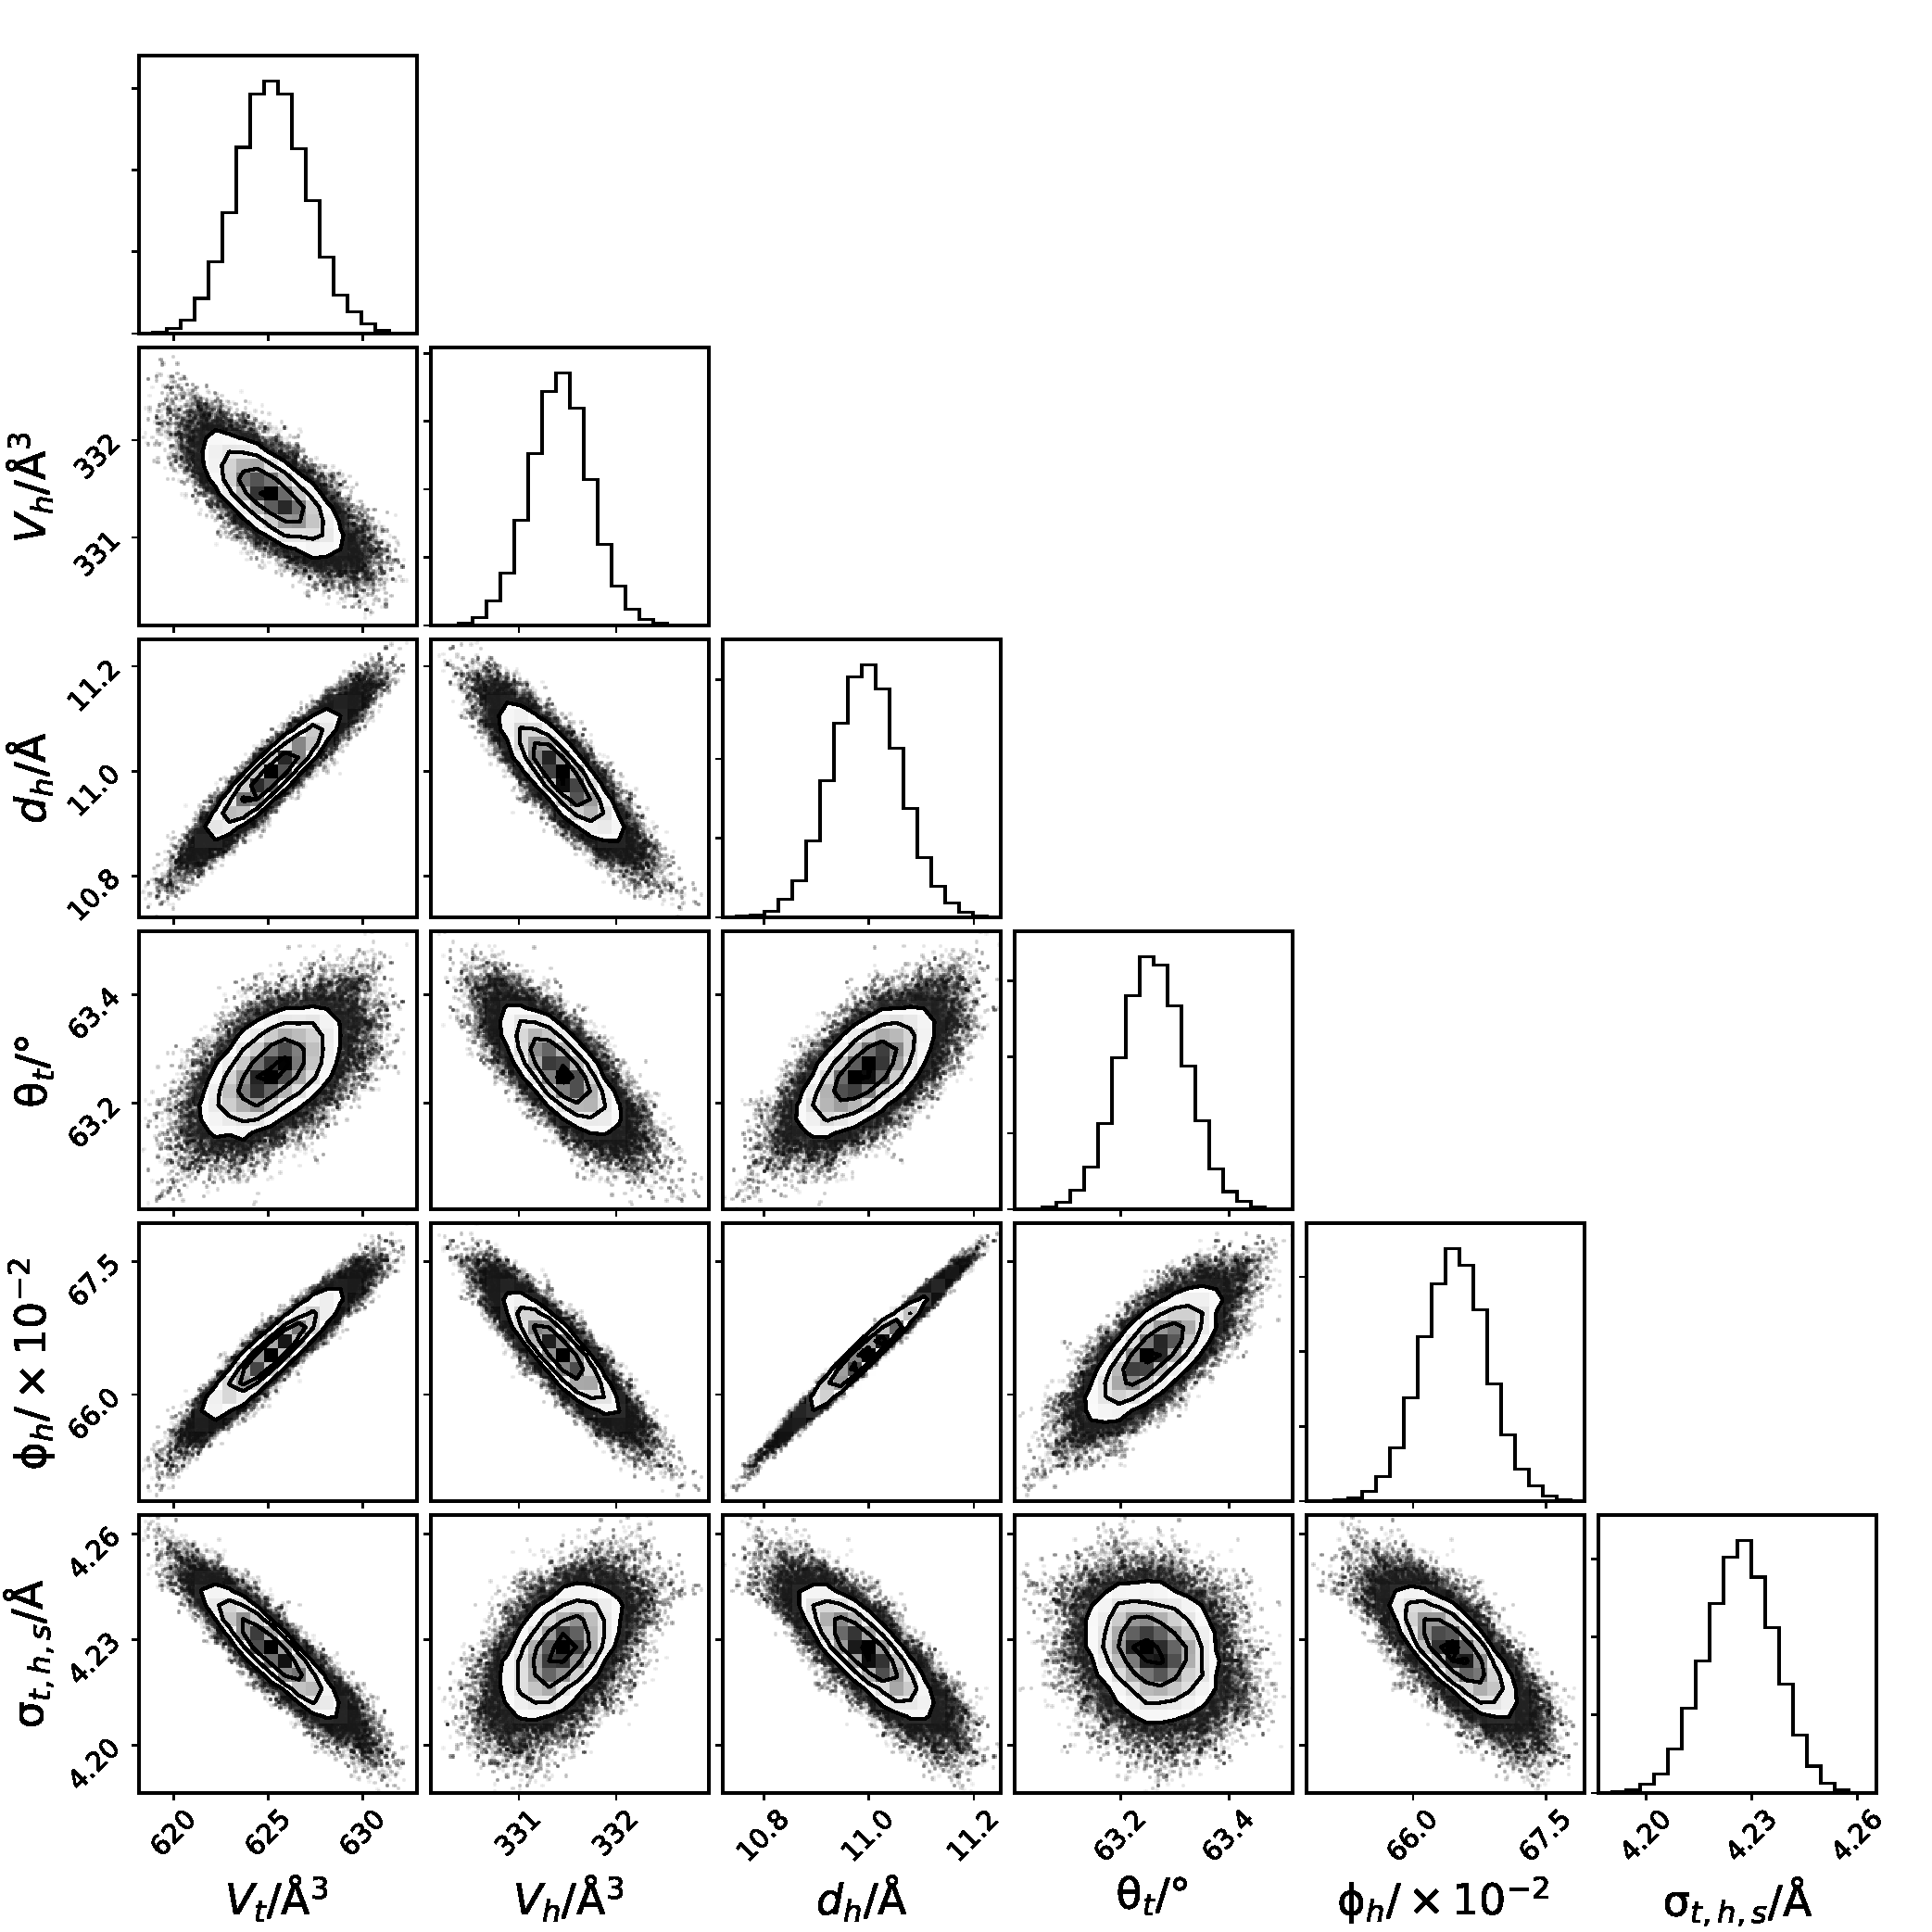
\includegraphics[width=0.50\textwidth]{figures/dlpc1_all_corner}
	\caption{The multi-parameter PDFs for the chemically-relevant model of DLPC X-ray reflectometry data at 20 mNm$^{-1}$. Source: Datasets, figure files and running/plotting scripts are available under CC-BY.\cite{mccluskey_2018}}
	\label{fig:dlpc2}
\end{figure}
\begin{figure}[h]
	\centering
	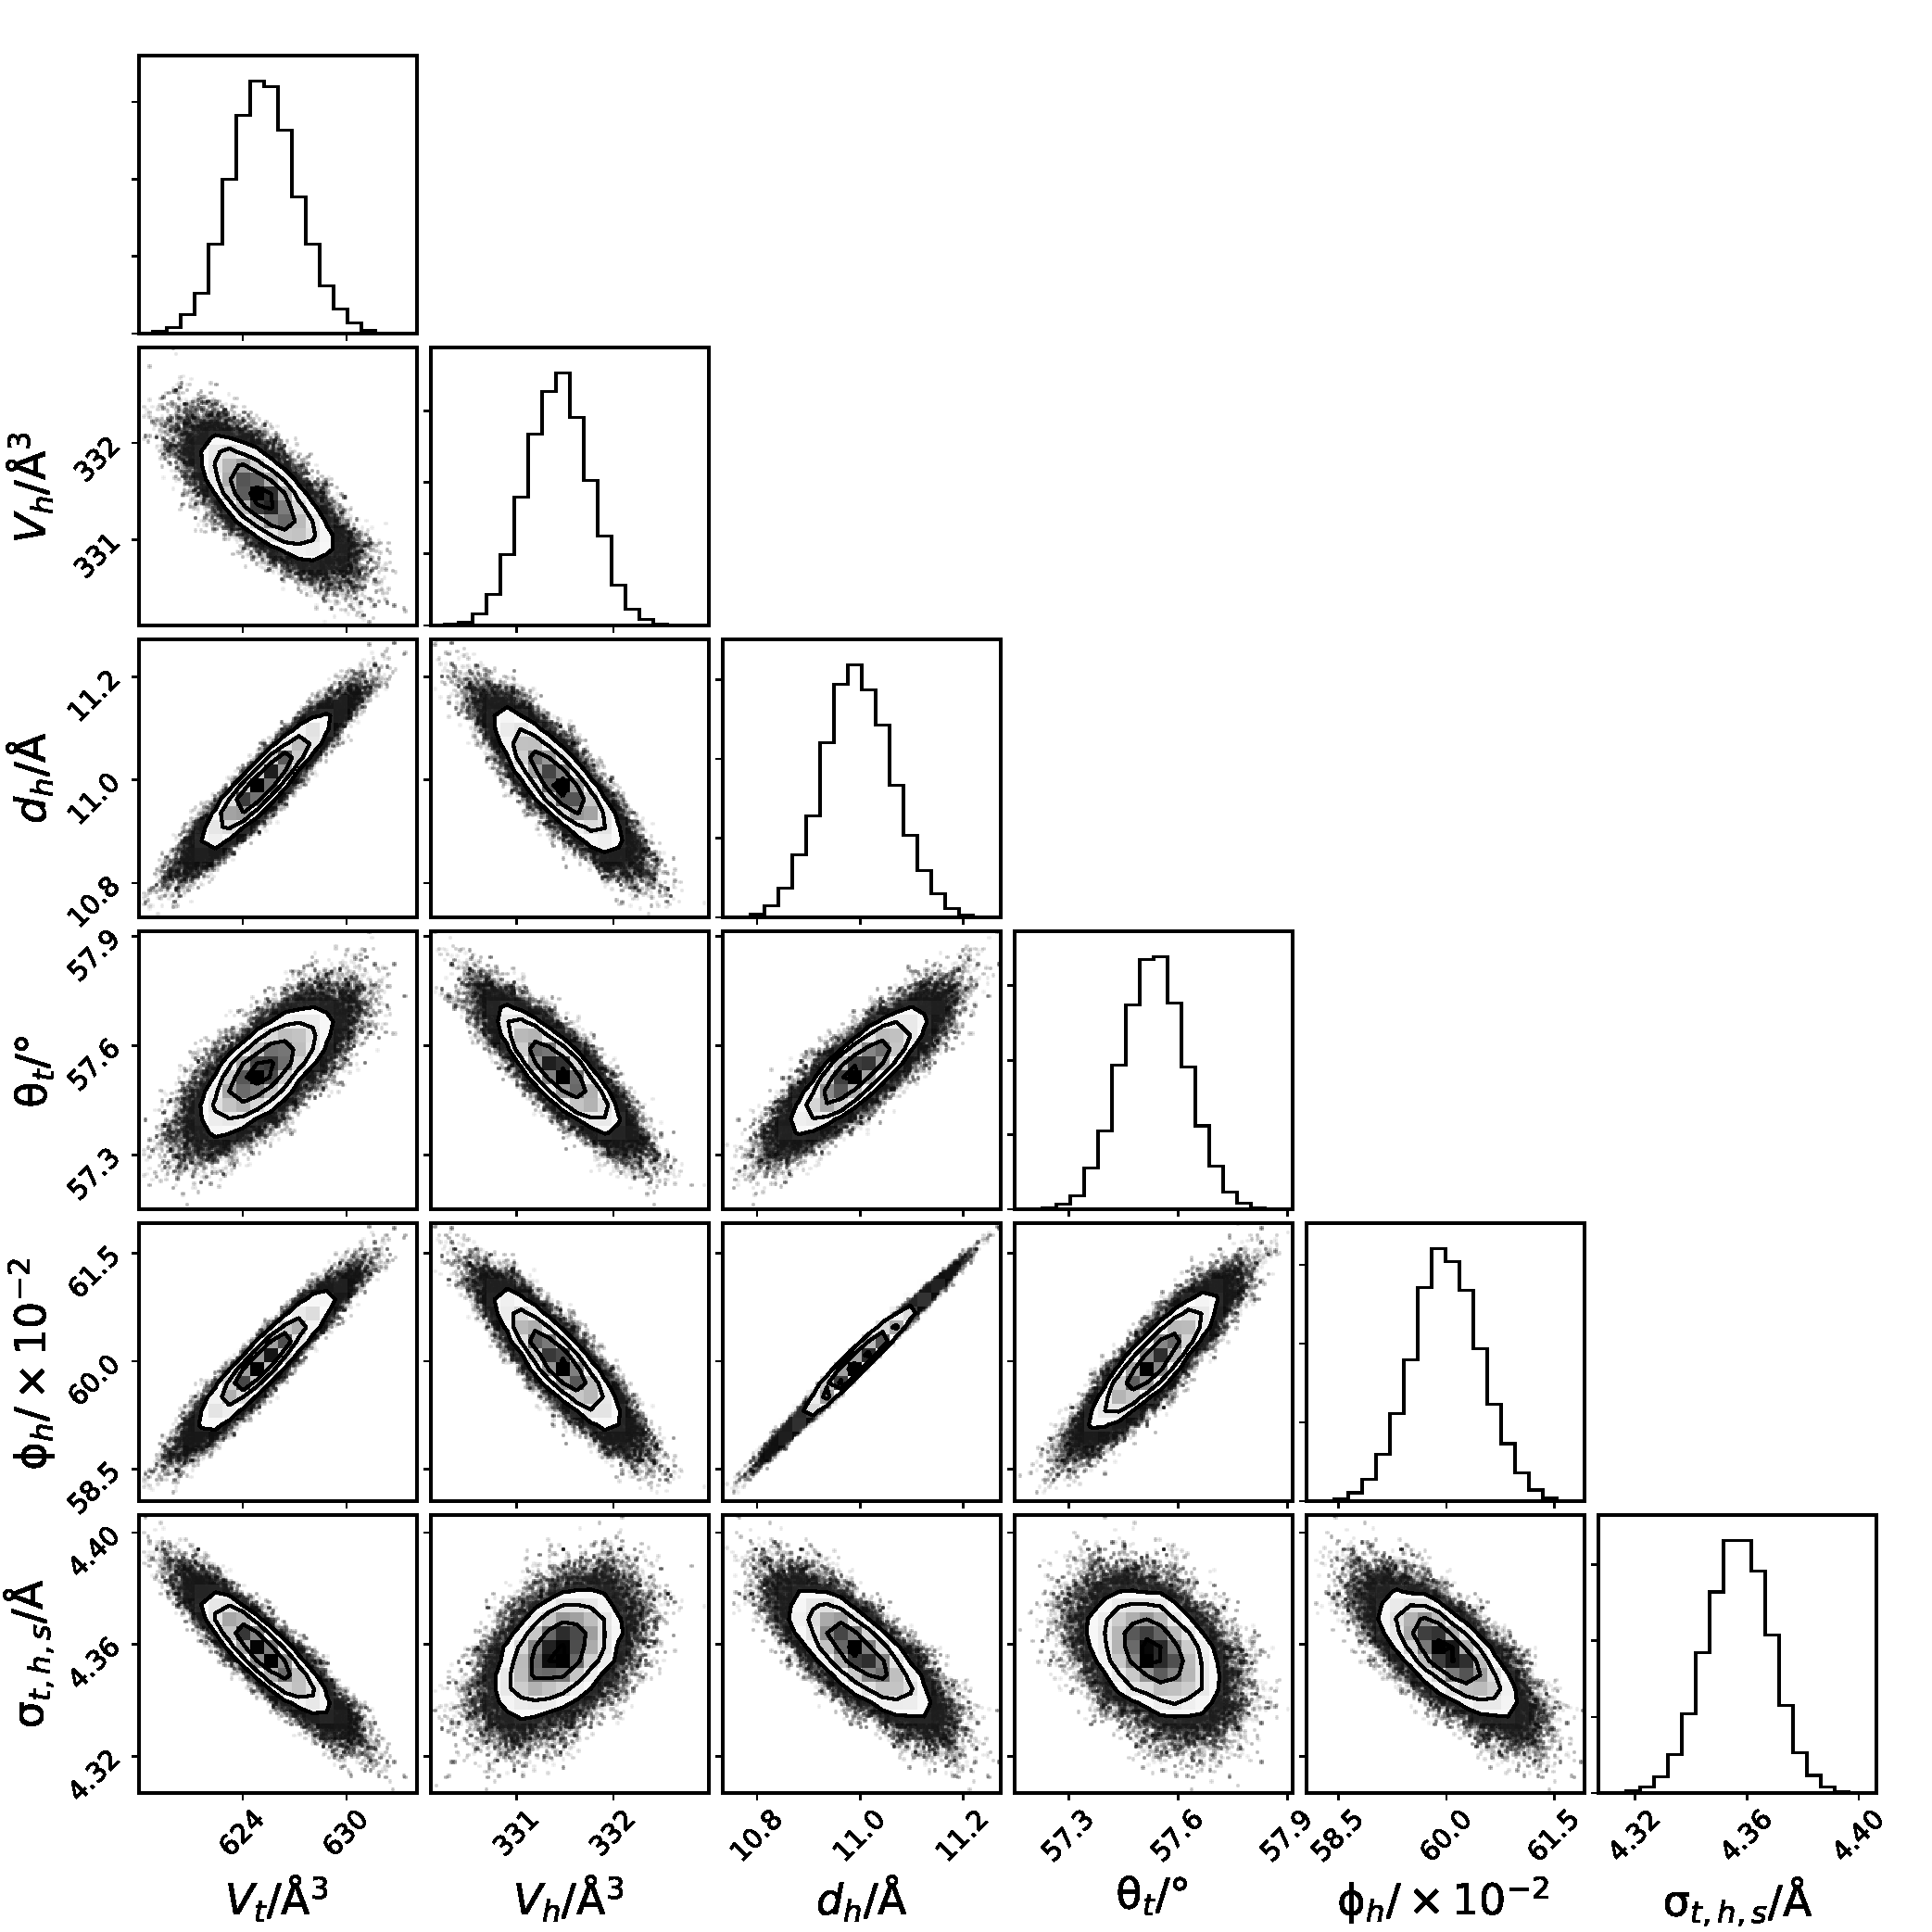
\includegraphics[width=0.50\textwidth]{figures/dlpc2_all_corner}
	\caption{The multi-parameter PDFs for the chemically-relevant model of DLPC X-ray reflectometry data at 25 mNm$^{-1}$. Source: Datasets, figure files and running/plotting scripts are available under CC-BY.\cite{mccluskey_2018}}
	\label{fig:dlpc3}
\end{figure}
\begin{figure}[h]
	\centering
	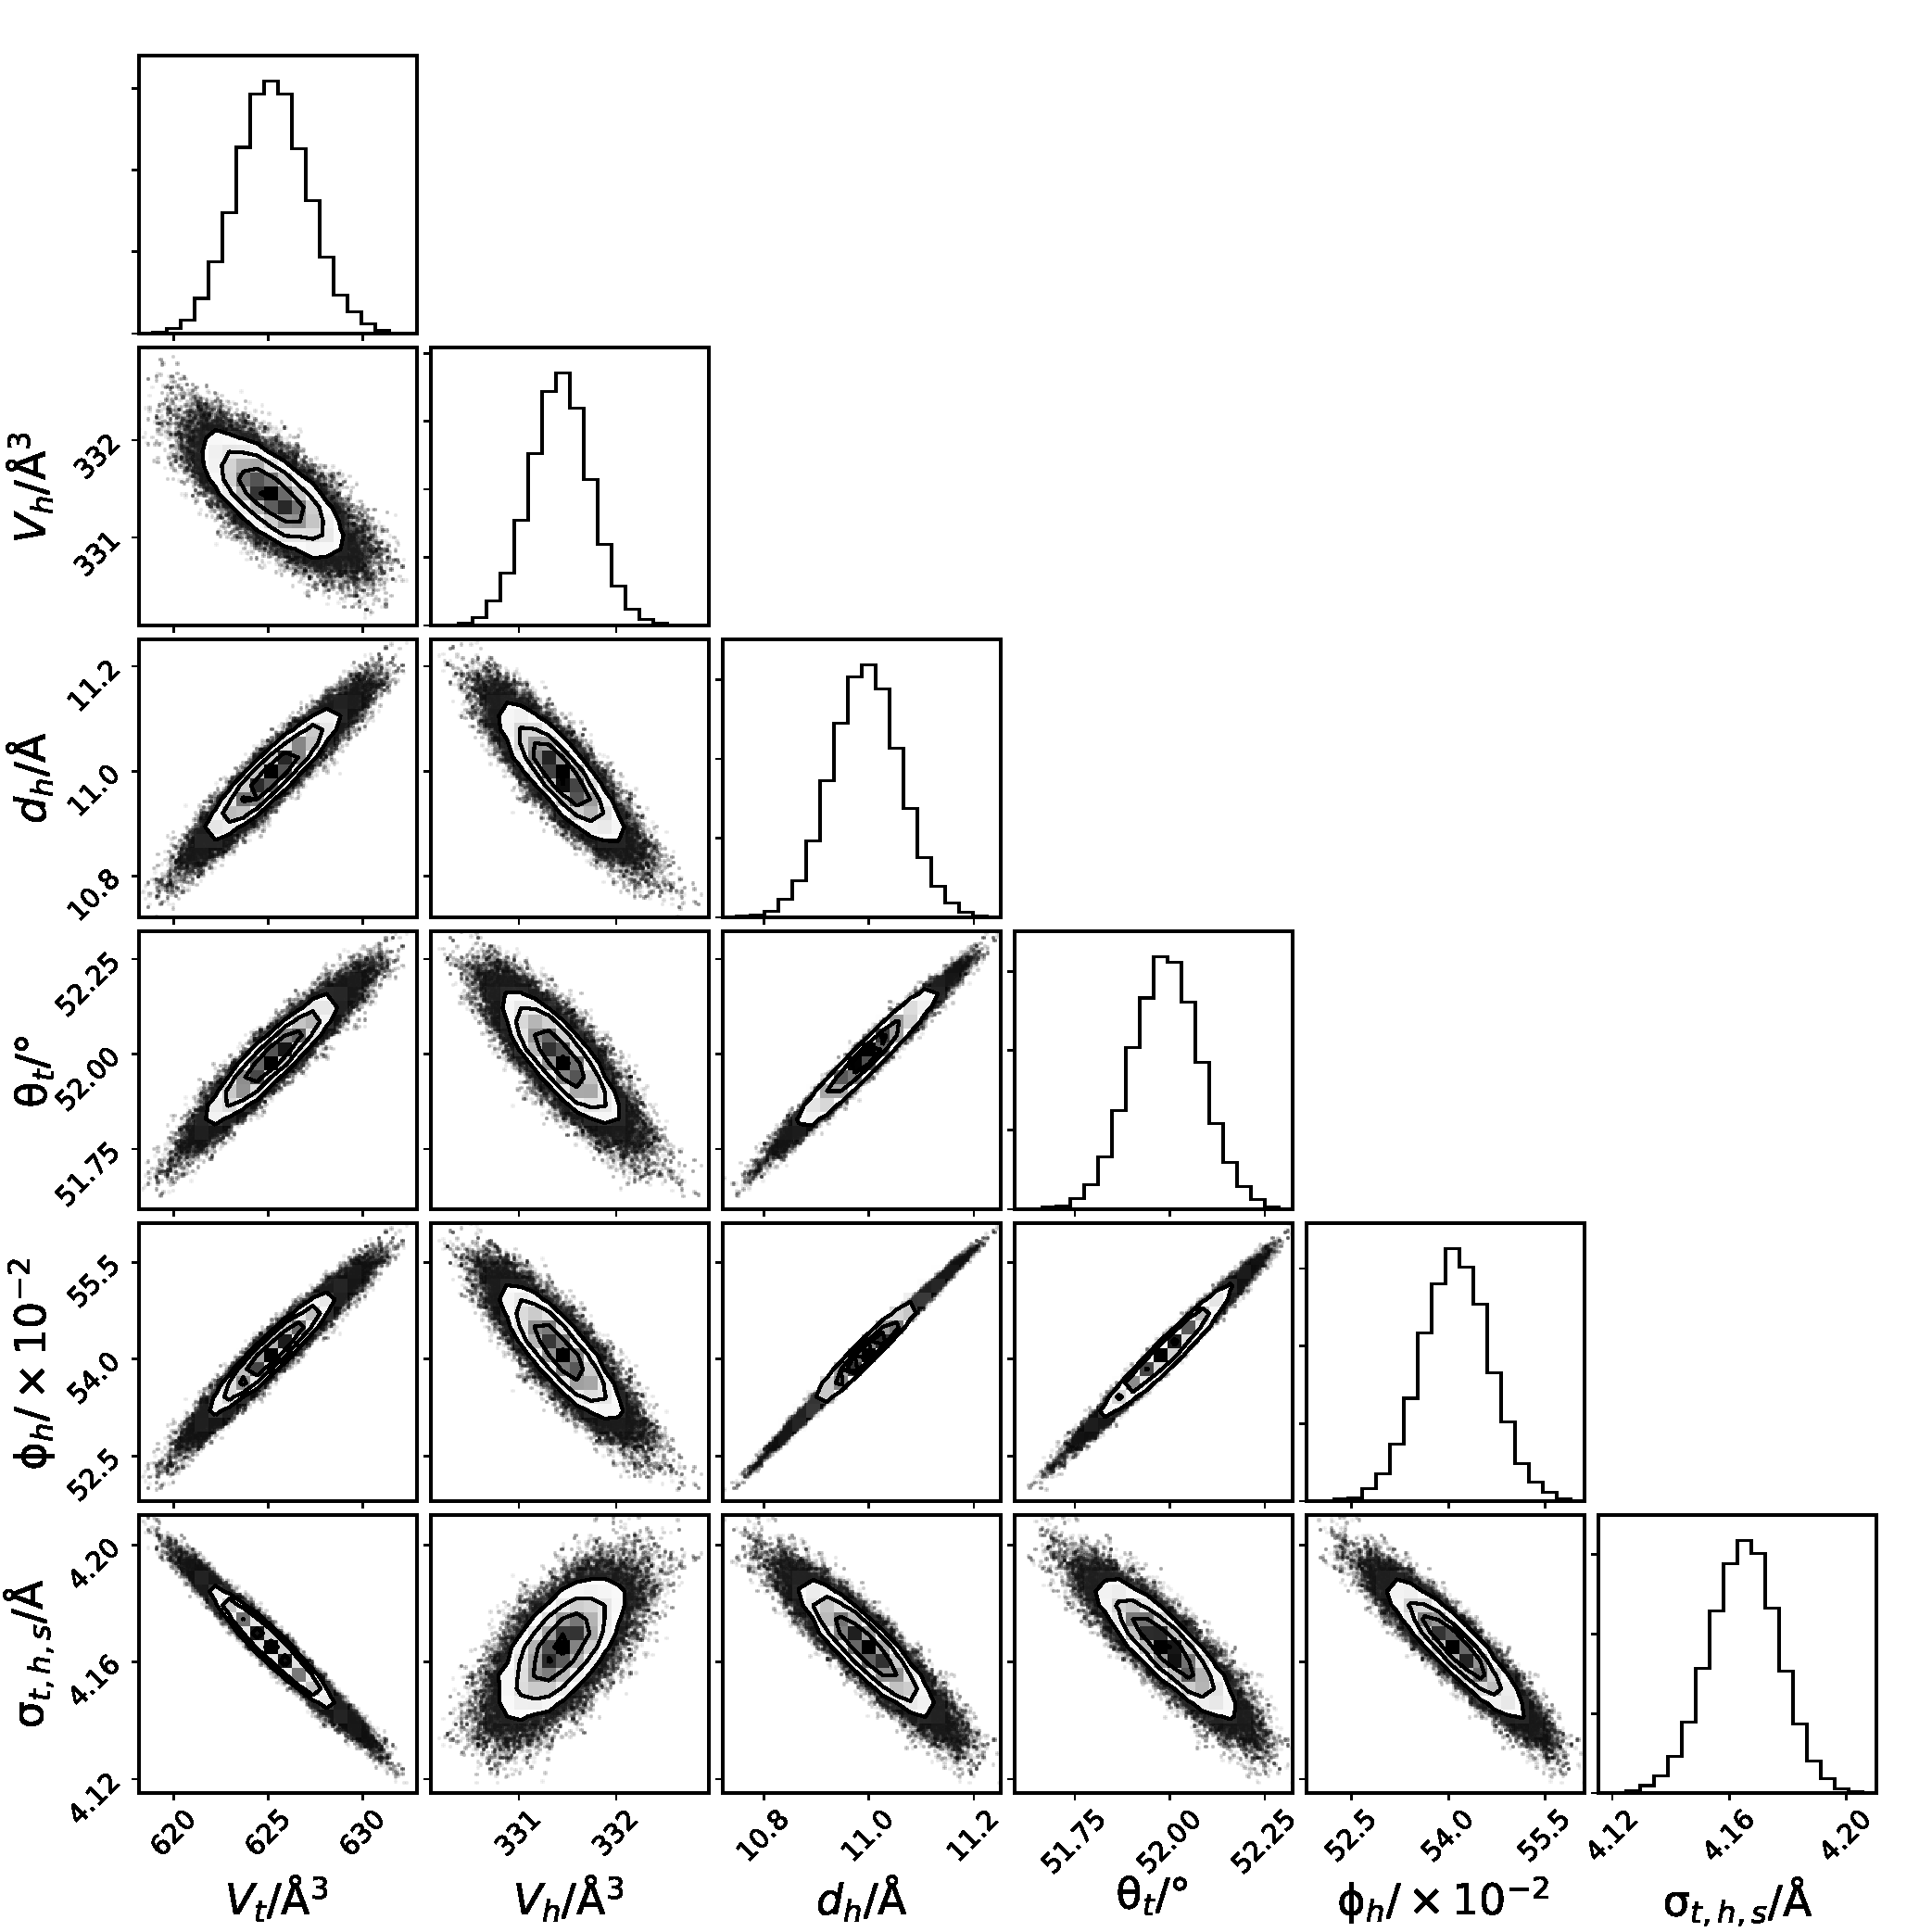
\includegraphics[width=0.50\textwidth]{figures/dlpc3_all_corner}
	\caption{The multi-parameter PDFs for the chemically-relevant model of DLPC X-ray reflectometry data at 30 mNm$^{-1}$. Source: Datasets, figure files and running/plotting scripts are available under CC-BY.\cite{mccluskey_2018}}
	\label{fig:dlpc4}
\end{figure}
\begin{figure}
	\centering
	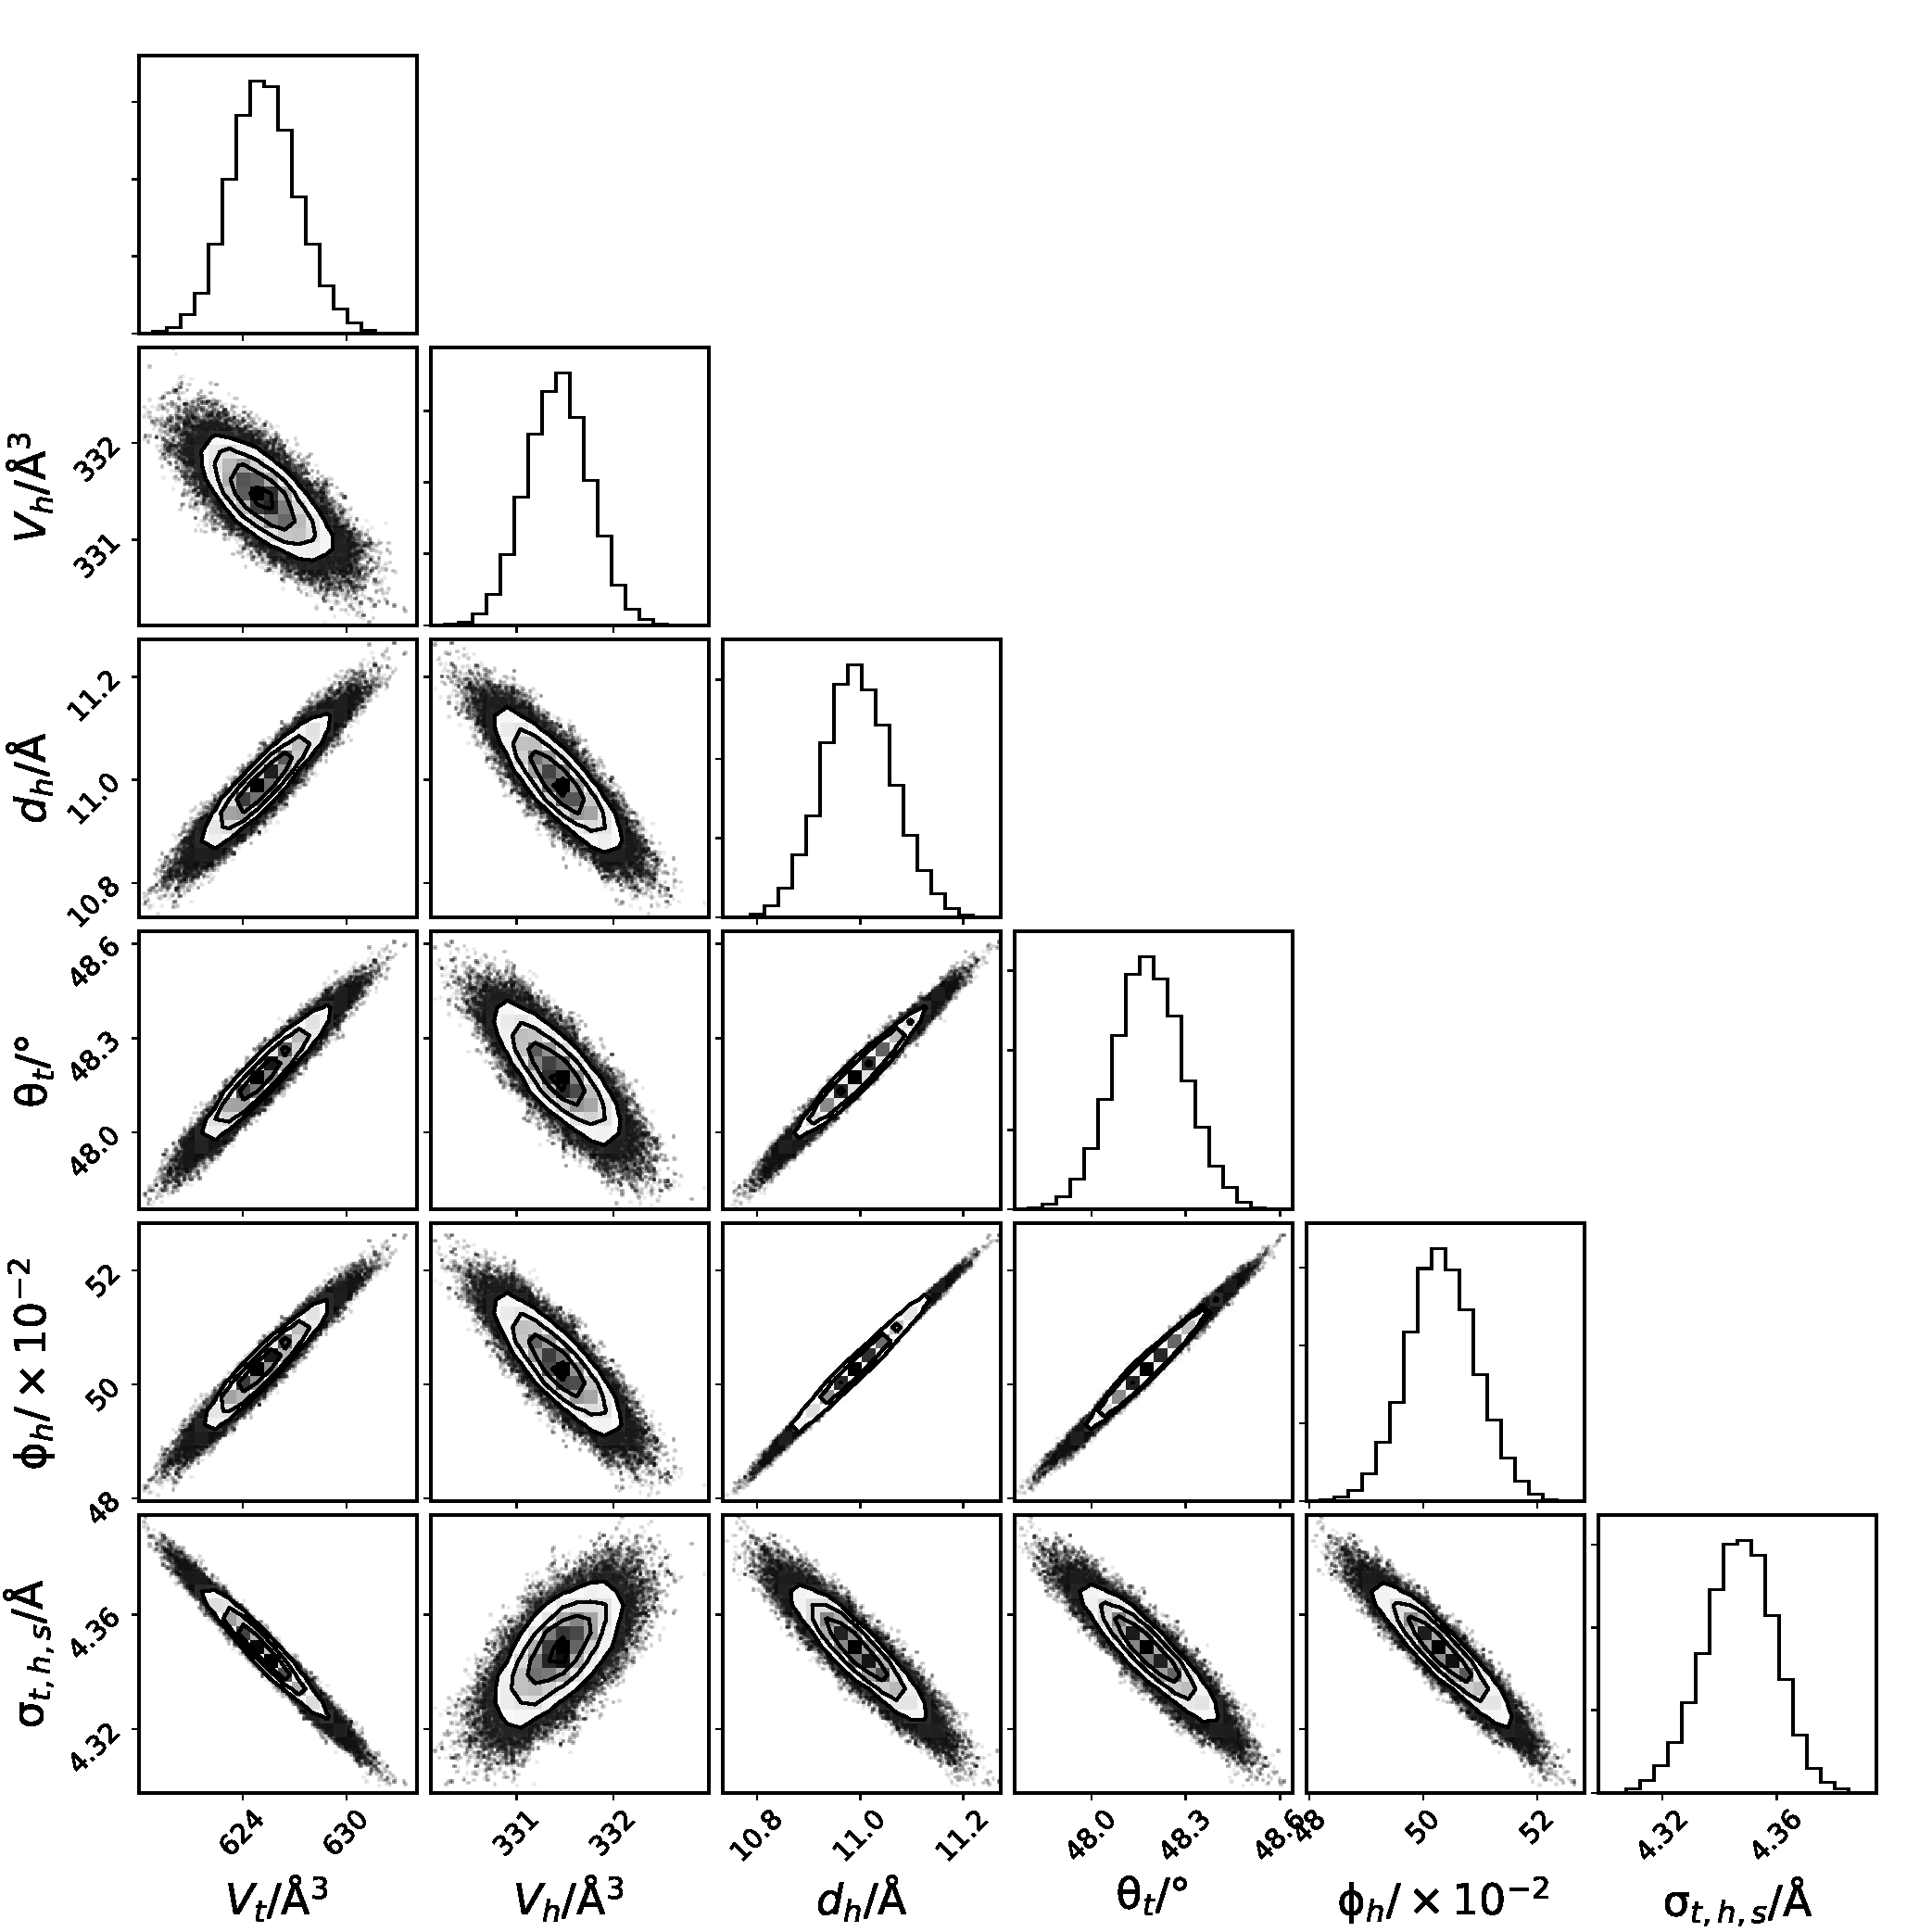
\includegraphics[width=0.50\textwidth]{figures/dlpc4_all_corner}
	\caption{The multi-parameter PDFs for the chemically-relevant model of DLPC X-ray reflectometry data at 35 mNm$^{-1}$. Source: Datasets, figure files and running/plotting scripts are available under CC-BY.\cite{mccluskey_2018}}
	\label{fig:dlpc5}
\end{figure}
\begin{figure}[h]
	\centering
	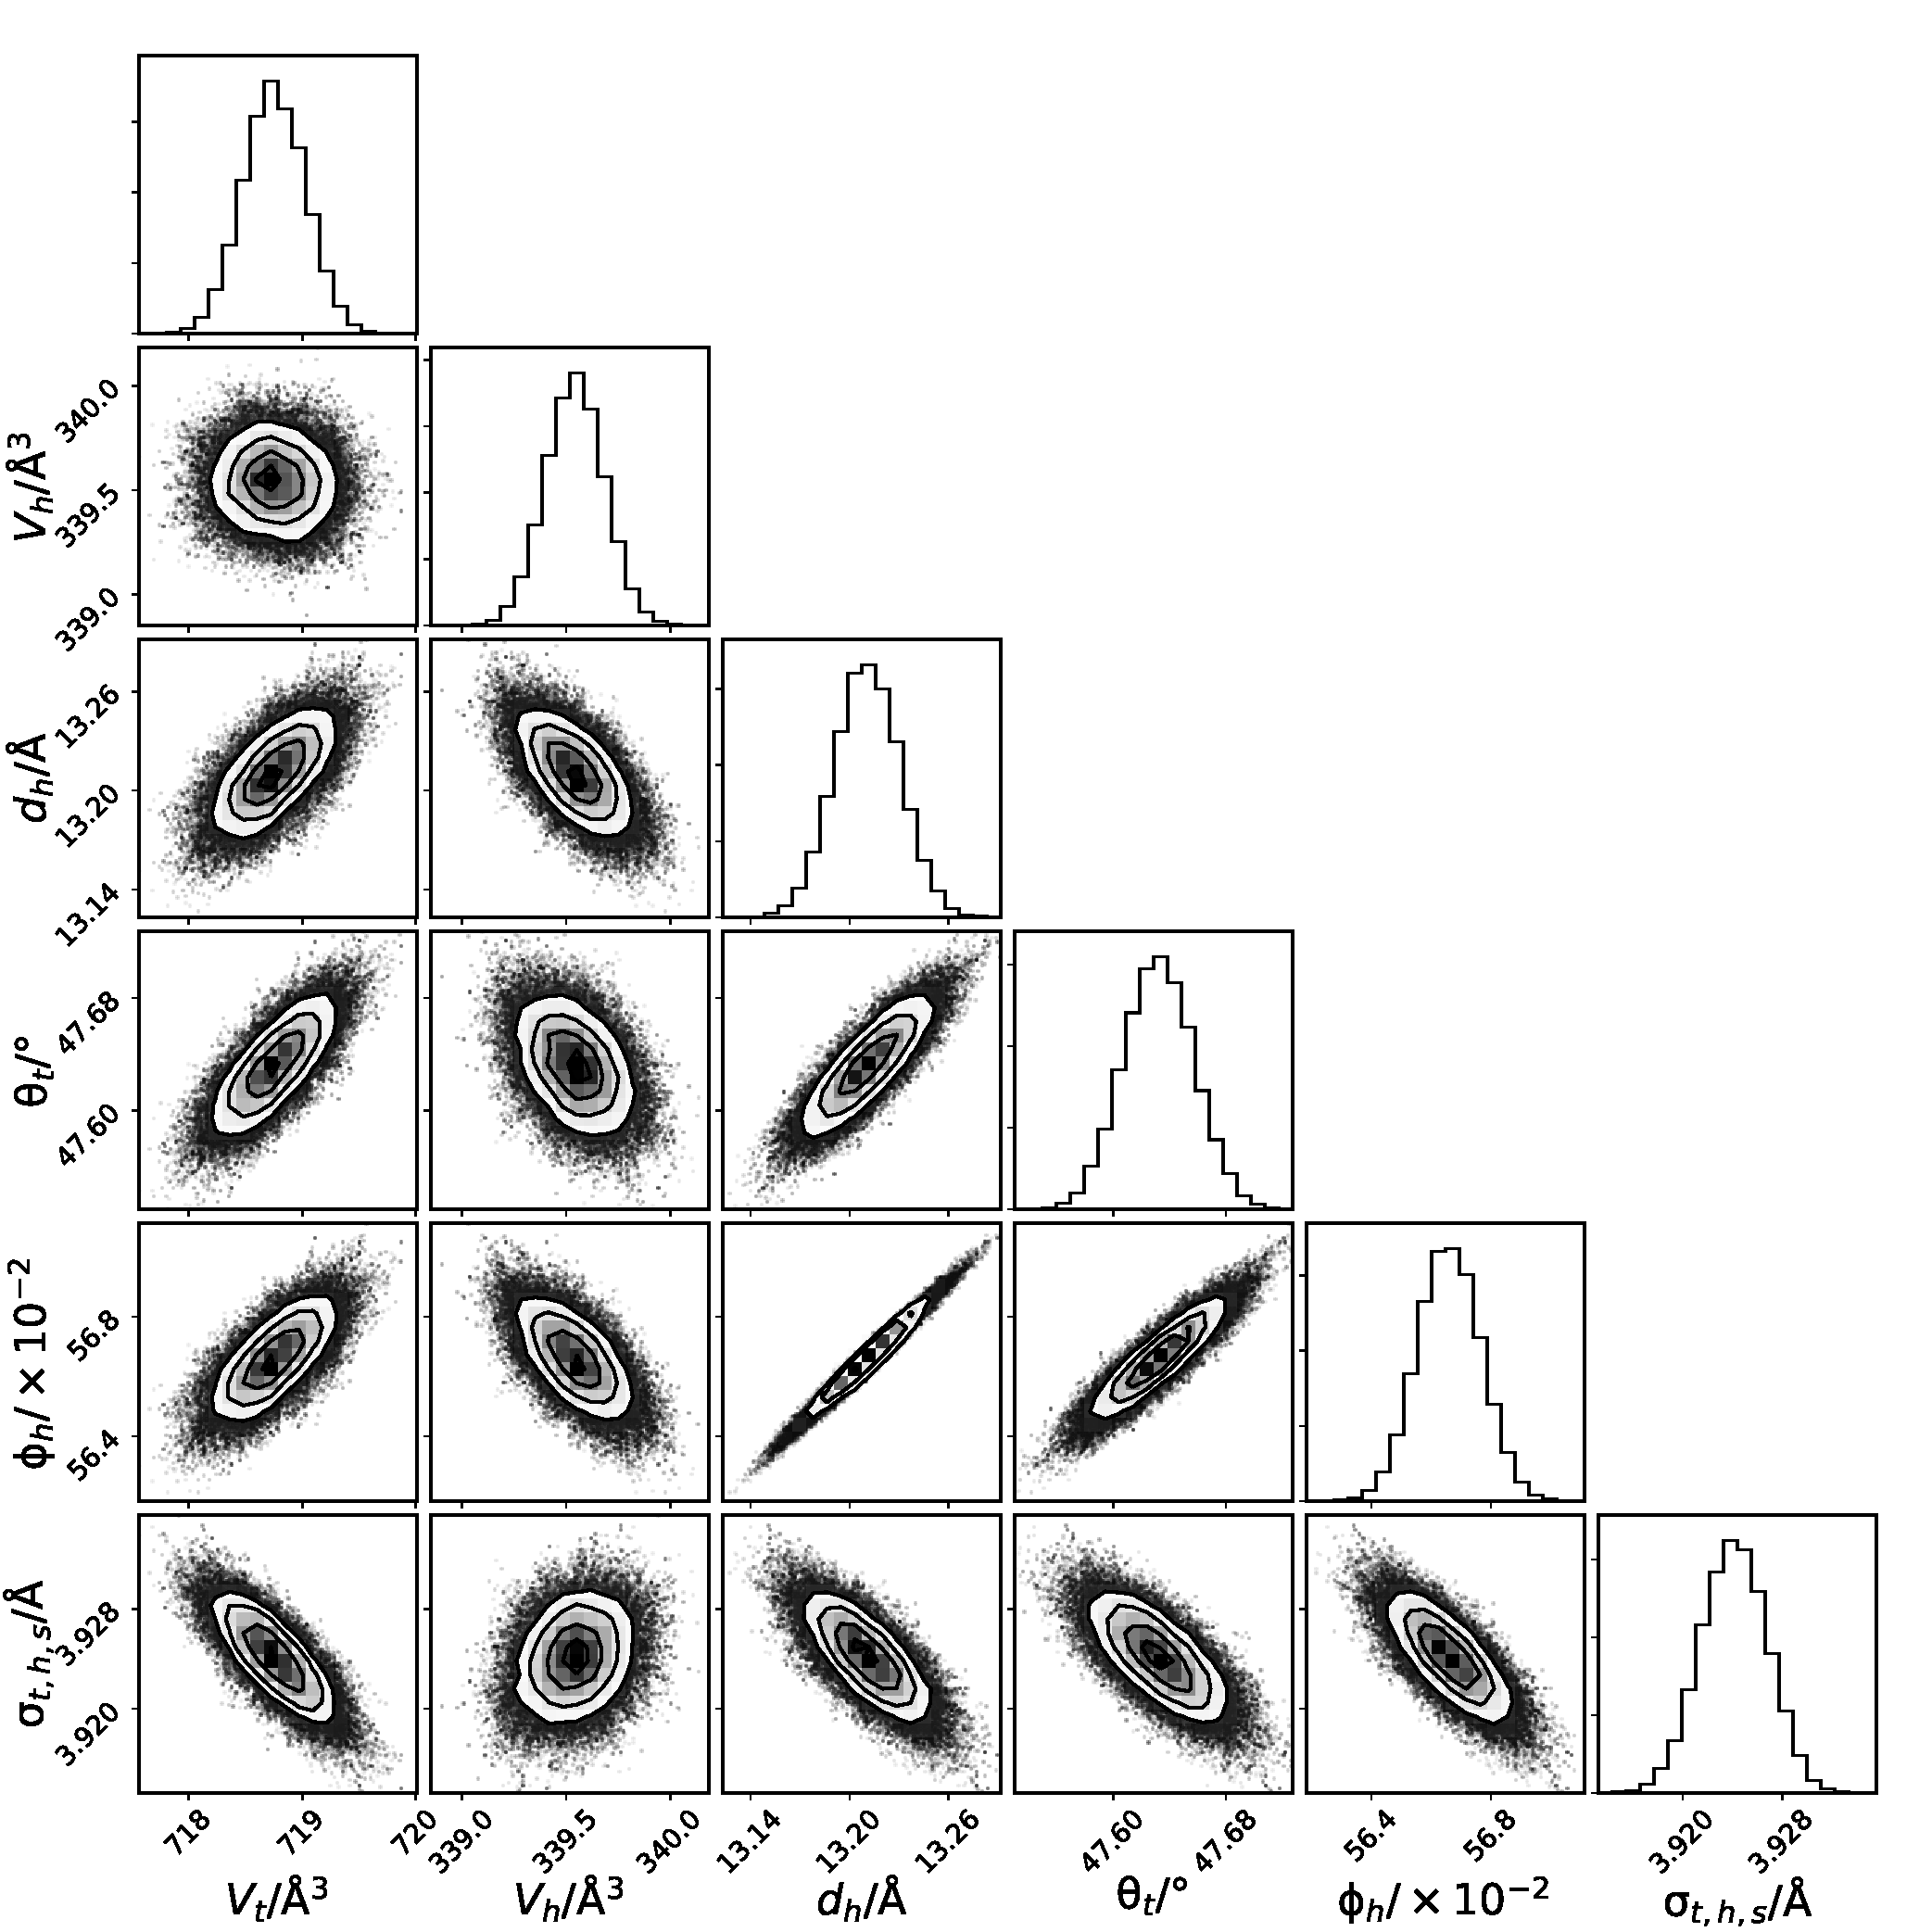
\includegraphics[width=0.50\textwidth]{figures/dmpc2_all_corner}
	\caption{The multi-parameter PDFs for the chemically-relevant model of DMPC X-ray reflectometry data at 20 mNm$^{-1}$. Source: Datasets, figure files and running/plotting scripts are available under CC-BY.\cite{mccluskey_2018}}
	\label{fig:dmpc2}
\end{figure}
\begin{figure}[h]
	\centering
	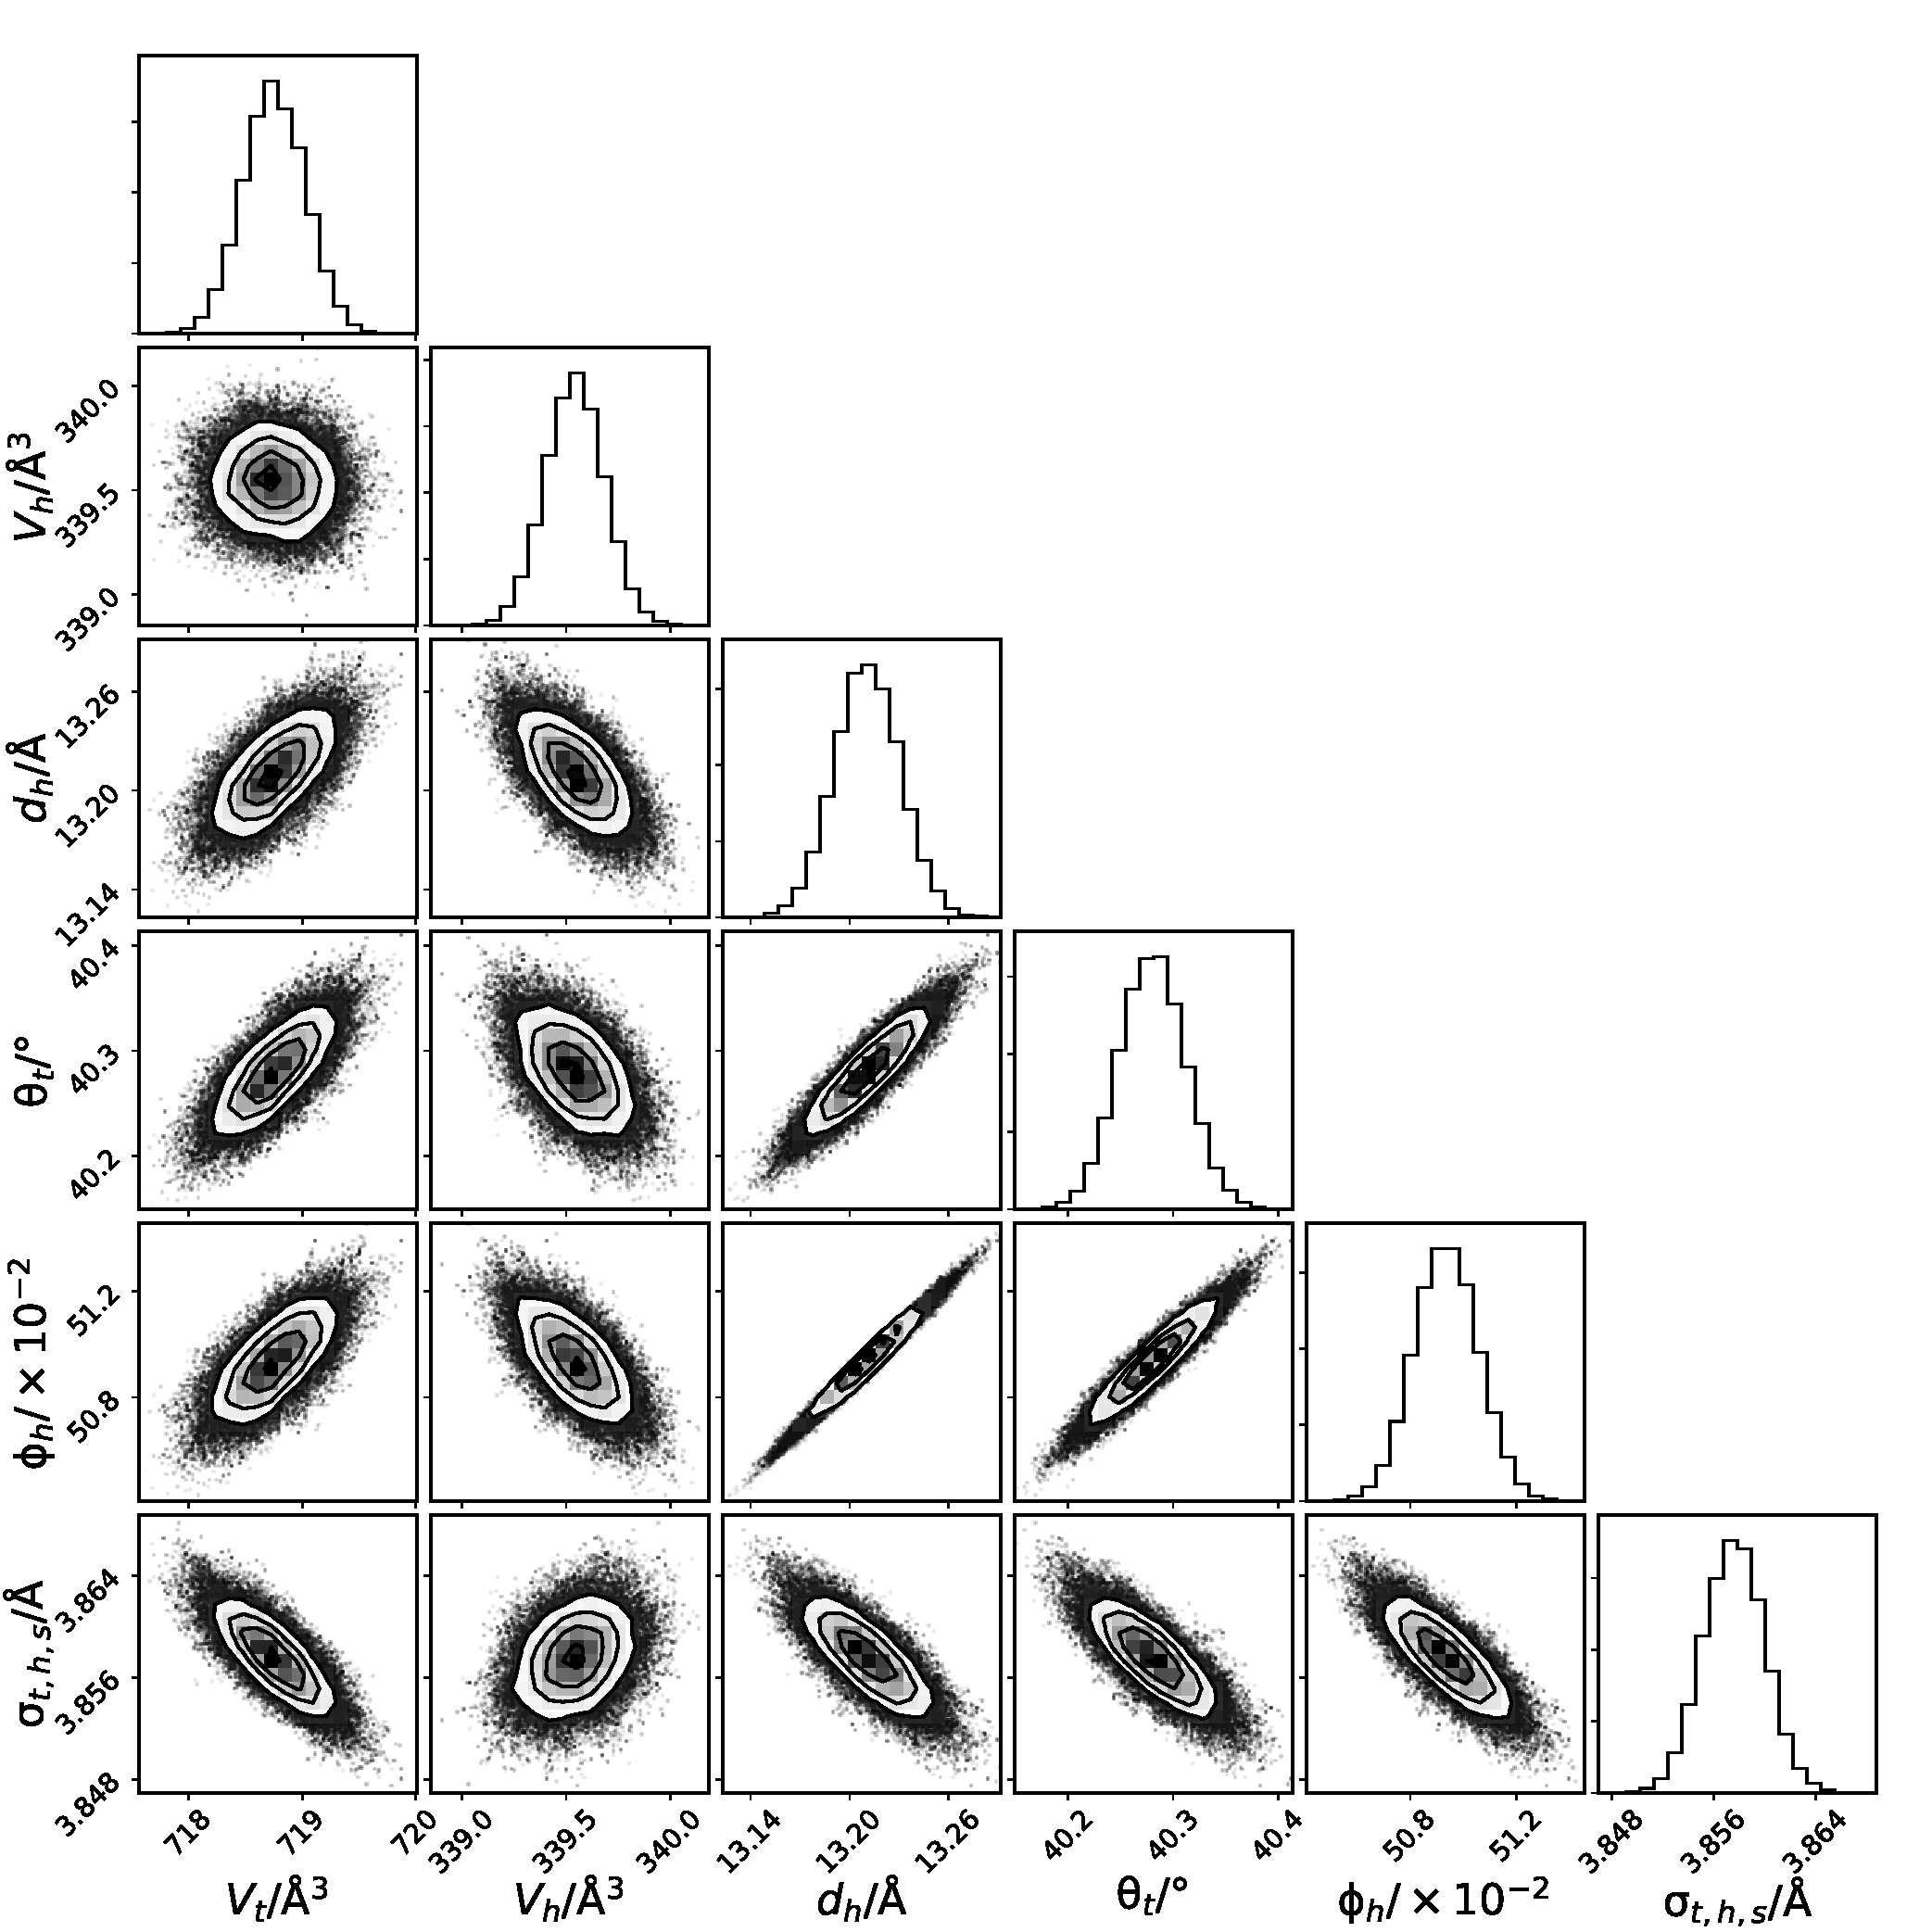
\includegraphics[width=0.50\textwidth]{figures/dmpc3_all_corner}
	\caption{The multi-parameter PDFs for the chemically-relevant model of DMPC X-ray reflectometry data at 25 mNm$^{-1}$. Source: Datasets, figure files and running/plotting scripts are available under CC-BY.\cite{mccluskey_2018}}
	\label{fig:dmpc3}
\end{figure}
\begin{figure}[h]
	\centering
	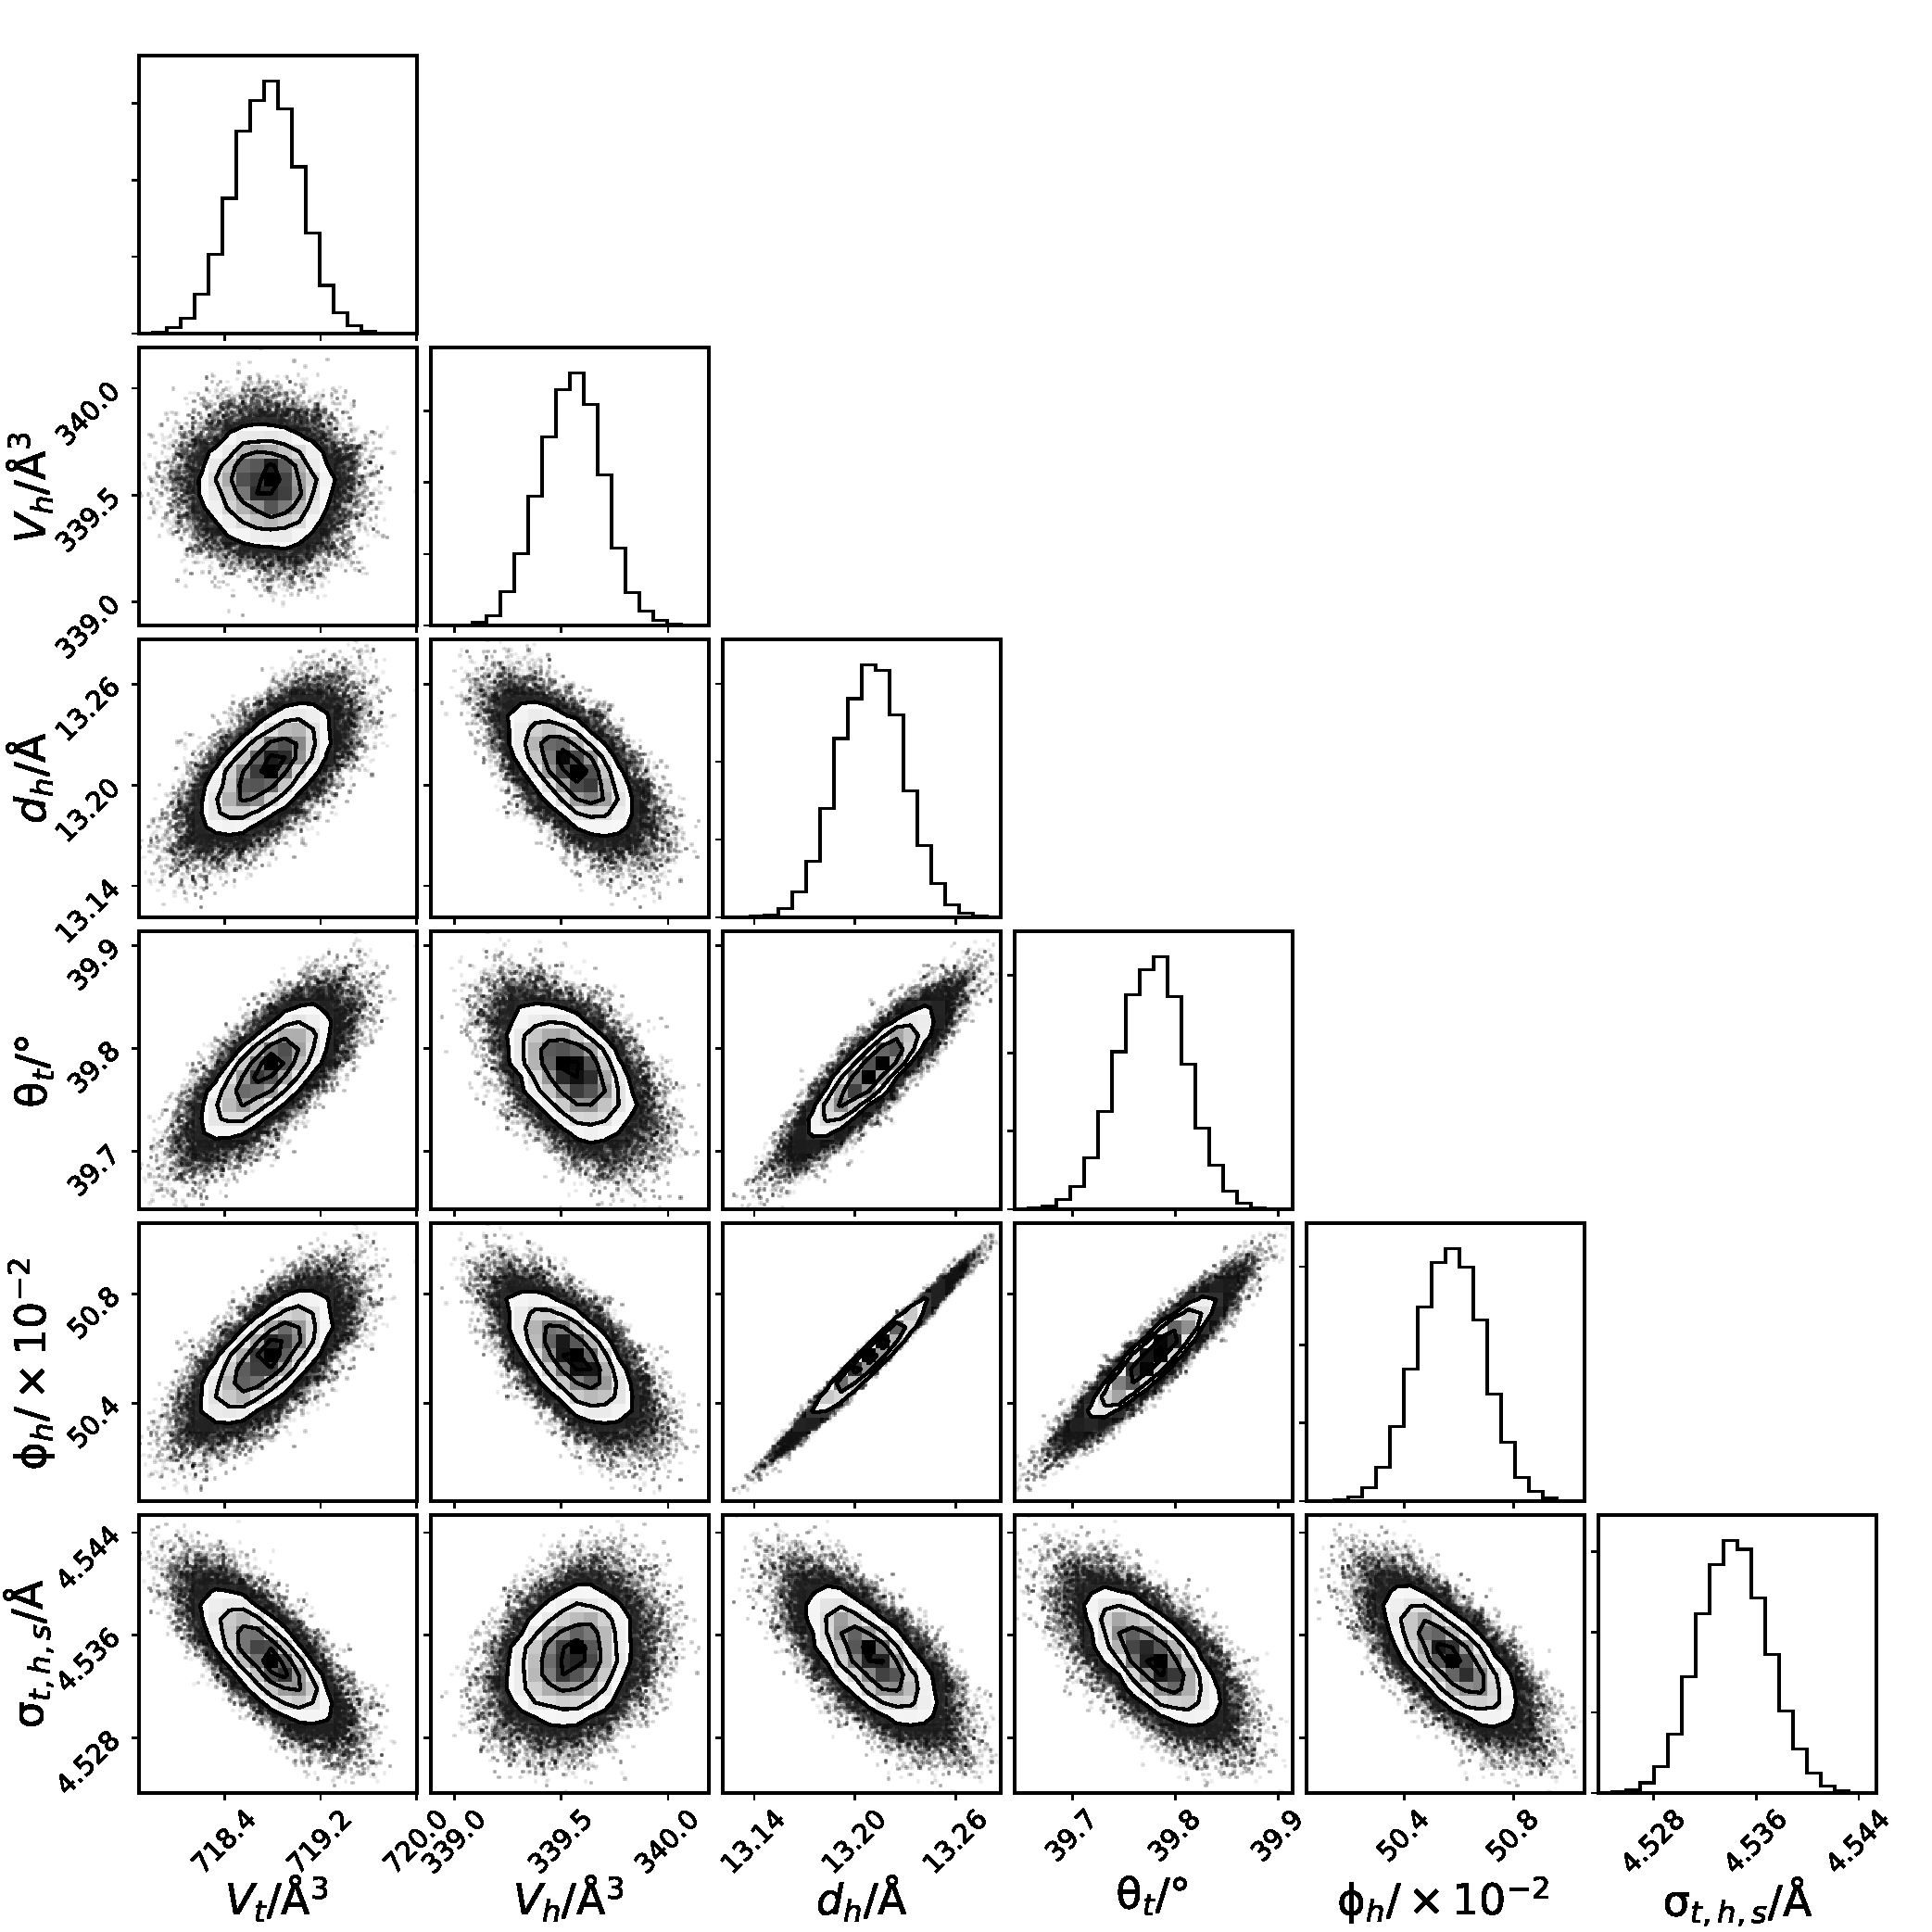
\includegraphics[width=0.50\textwidth]{figures/dmpc4_all_corner}
	\caption{The multi-parameter PDFs for the chemically-relevant model of DMPC X-ray reflectometry data at 30 mNm$^{-1}$. Source: Datasets, figure files and running/plotting scripts are available under CC-BY.\cite{mccluskey_2018}}
	\label{fig:dmpc4}
\end{figure}
\begin{figure}
	\centering
	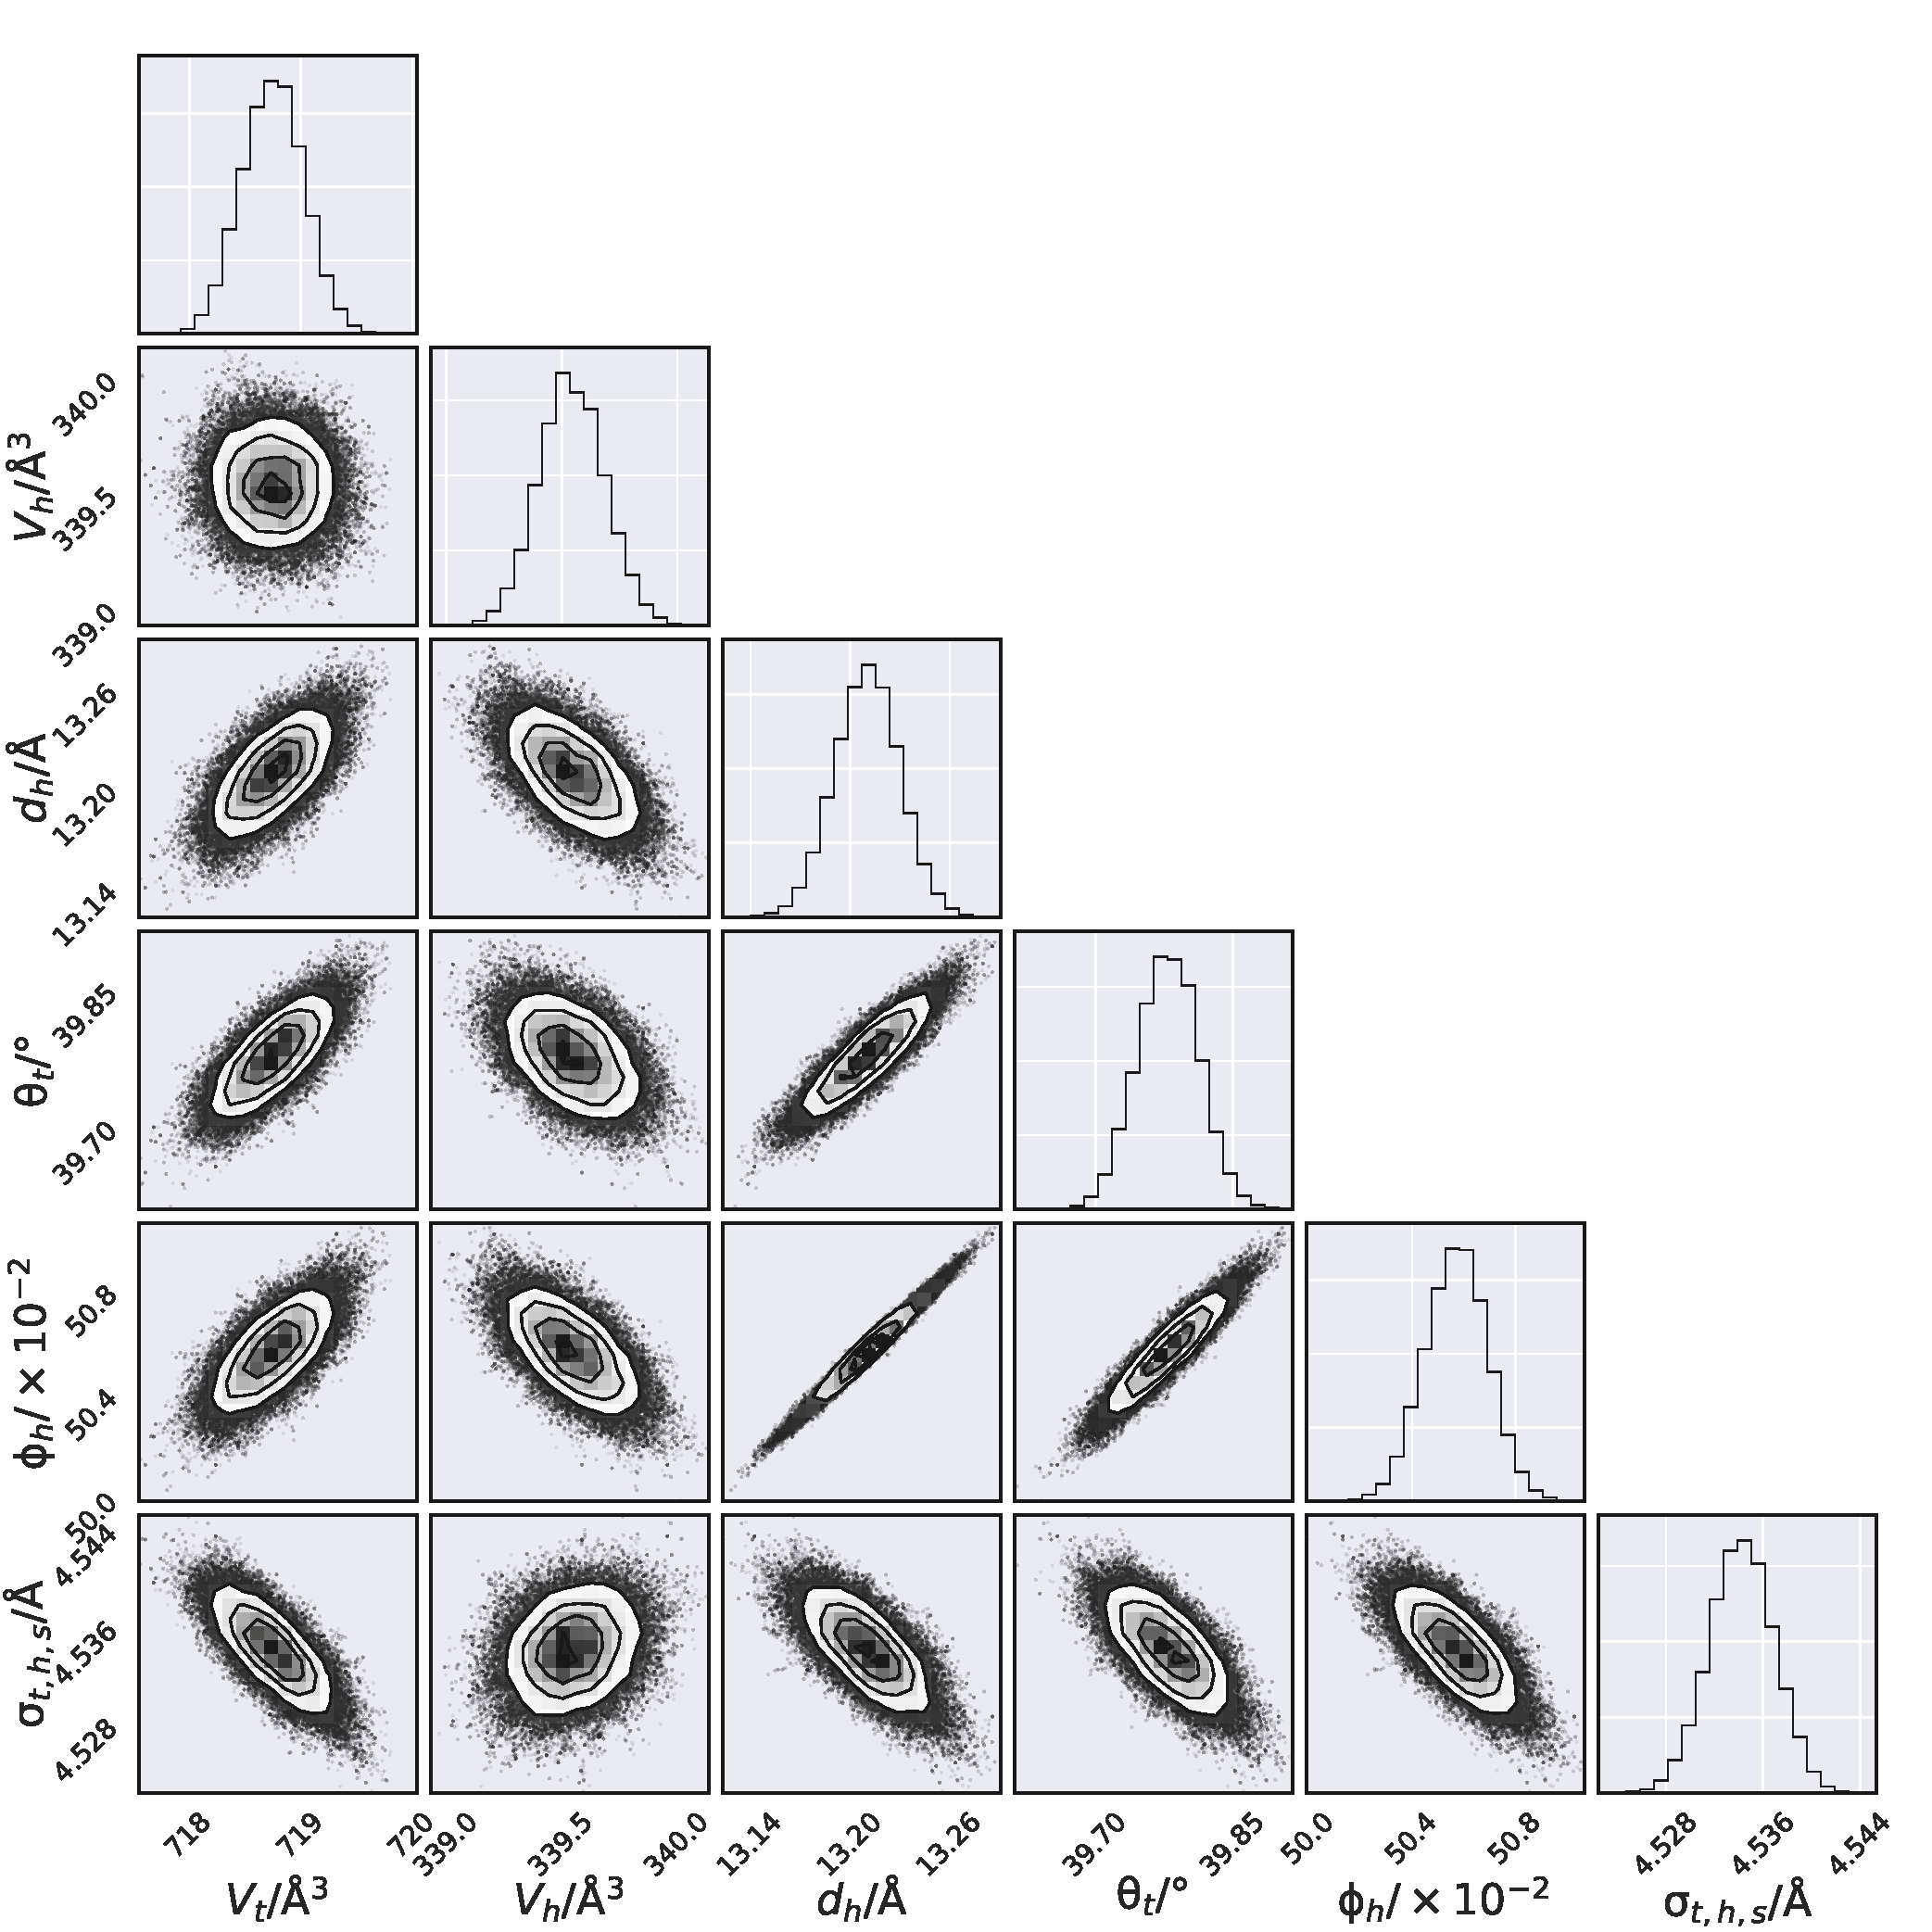
\includegraphics[width=0.50\textwidth]{figures/dmpc5_all_corner}
	\caption{The multi-parameter PDFs for the chemically-relevant model of DMPC X-ray reflectometry data at 40 mNm$^{-1}$. Source: Datasets, figure files and running/plotting scripts are available under CC-BY.\cite{mccluskey_2018}}
	\label{fig:dmpc5}
\end{figure}
\begin{figure}[h]
	\centering
	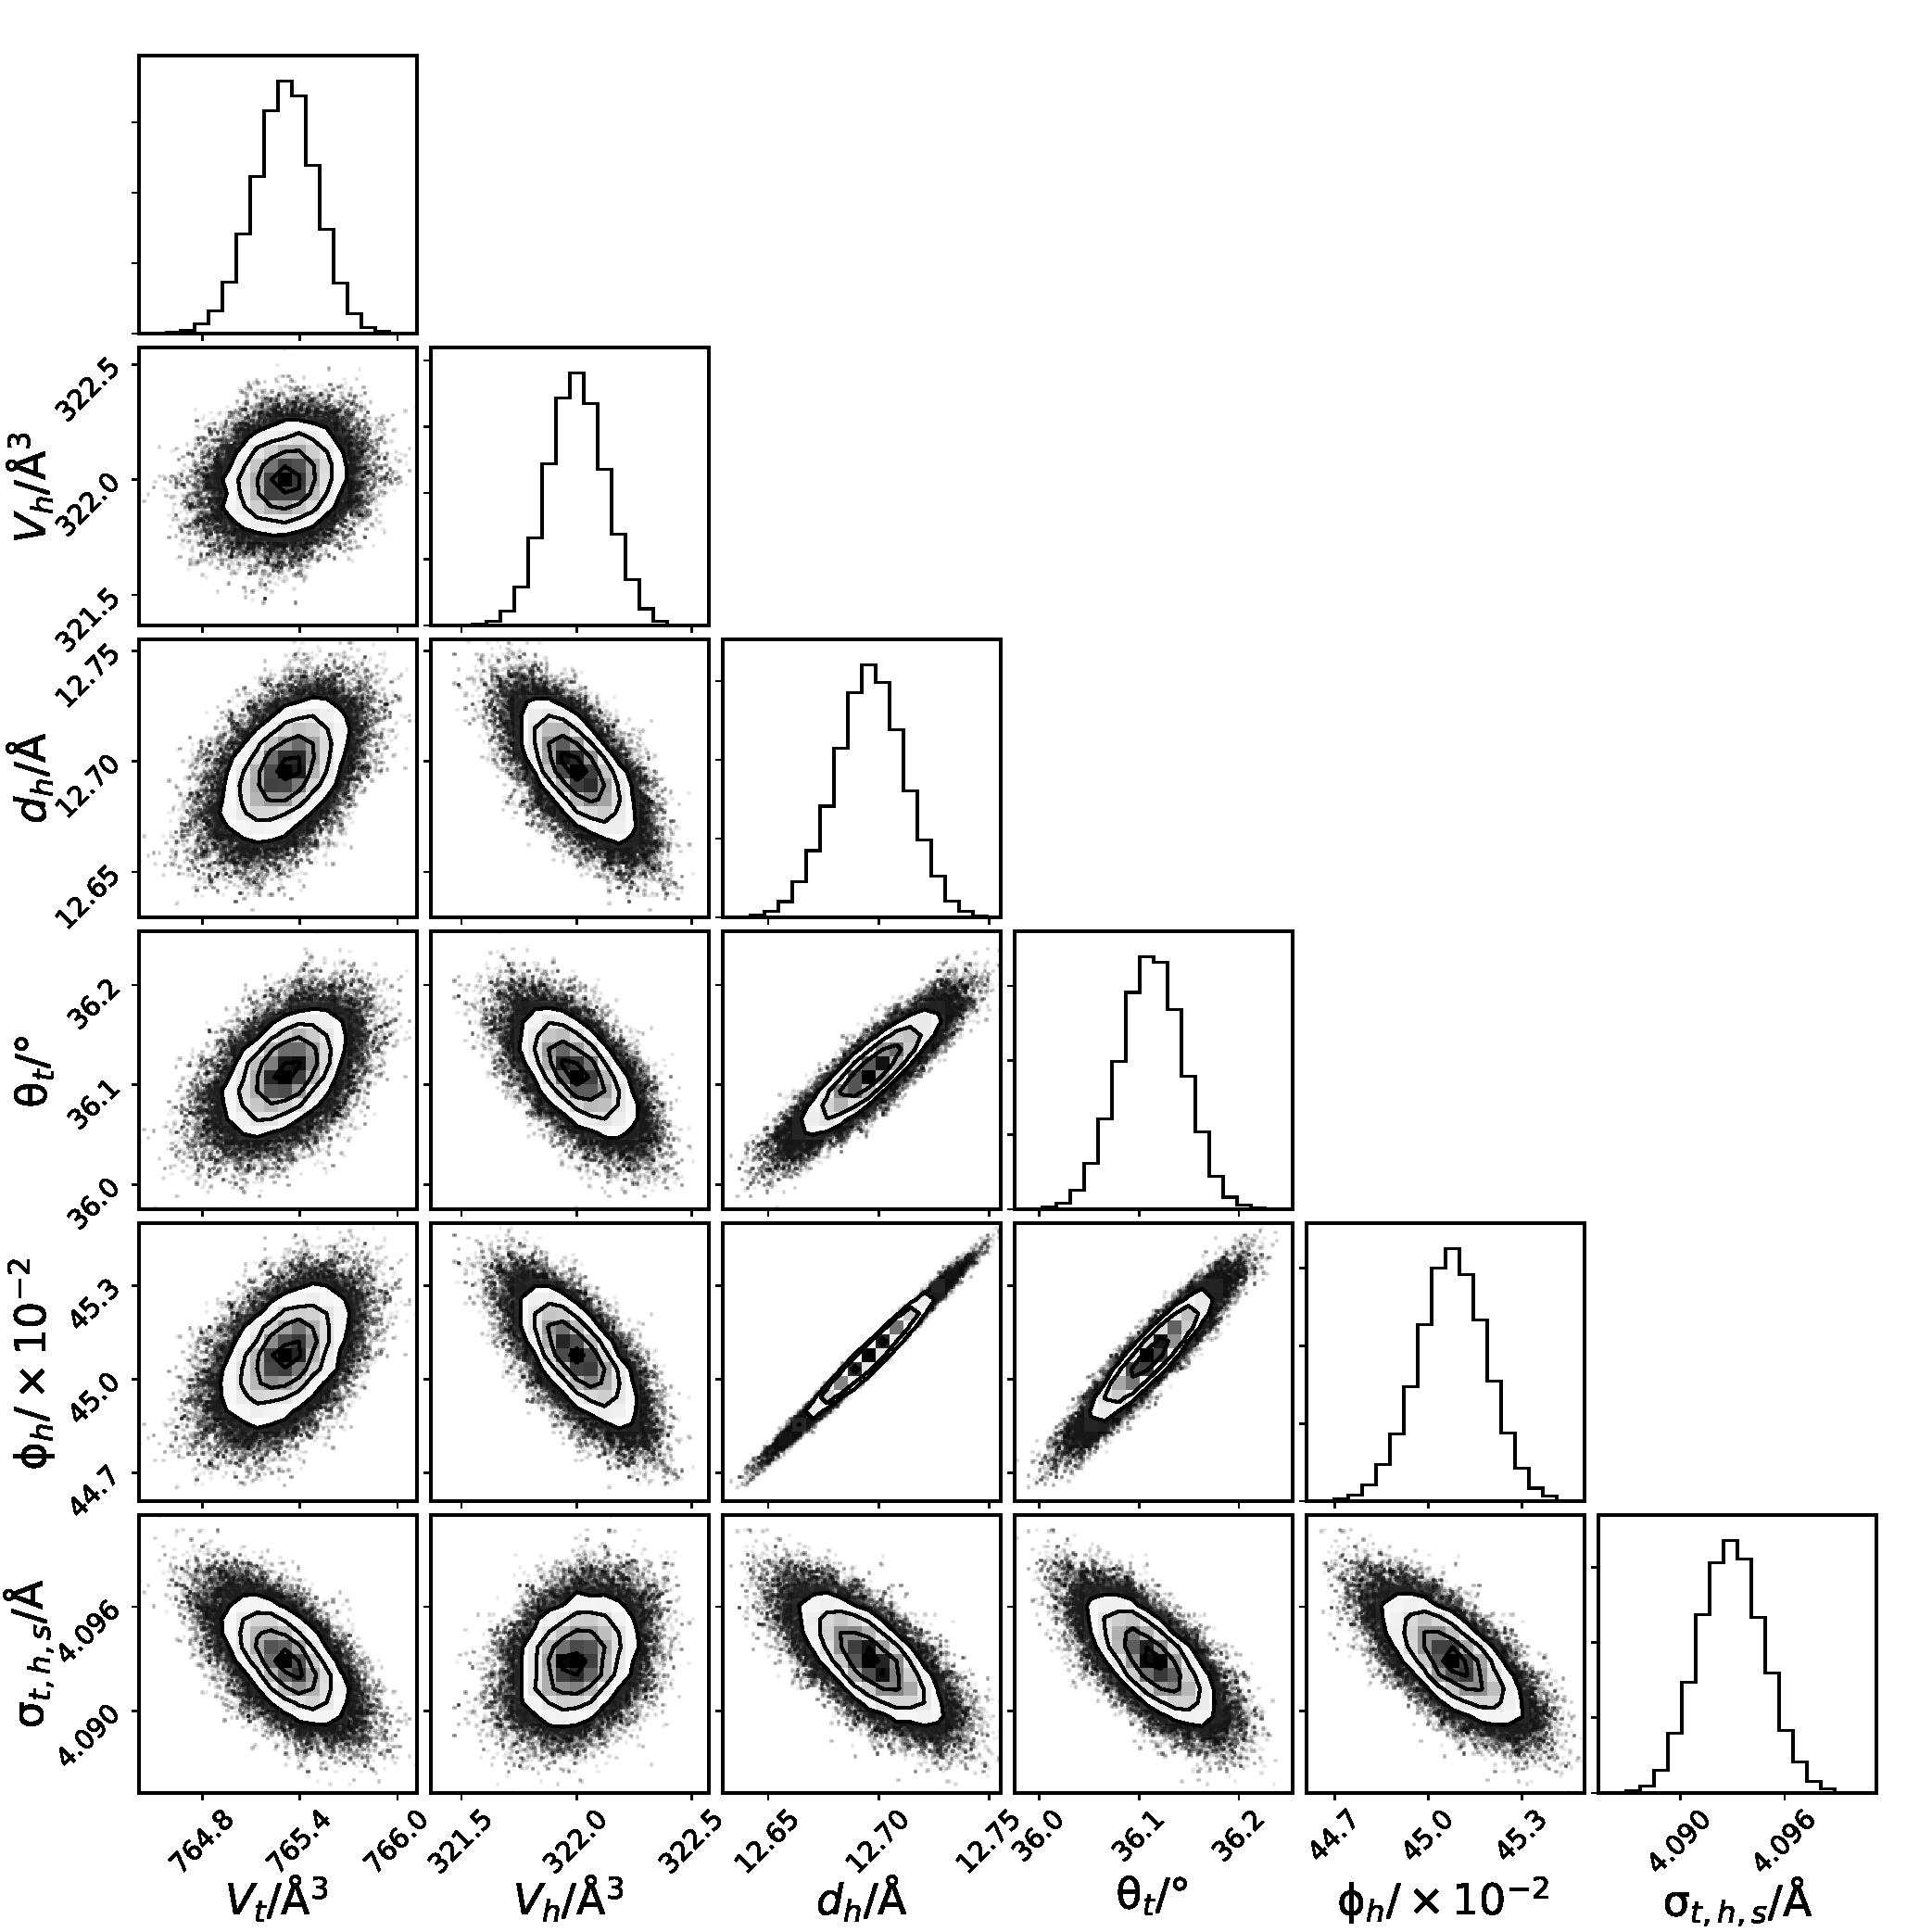
\includegraphics[width=0.50\textwidth]{figures/dppc2_all_corner}
	\caption{The multi-parameter PDFs for the chemically-relevant model of DPPC X-ray reflectometry data at 15 mNm$^{-1}$. Source: Datasets, figure files and running/plotting scripts are available under CC-BY.\cite{mccluskey_2018}}
	\label{fig:dppc2}
\end{figure}
\begin{figure}[h]
	\centering
	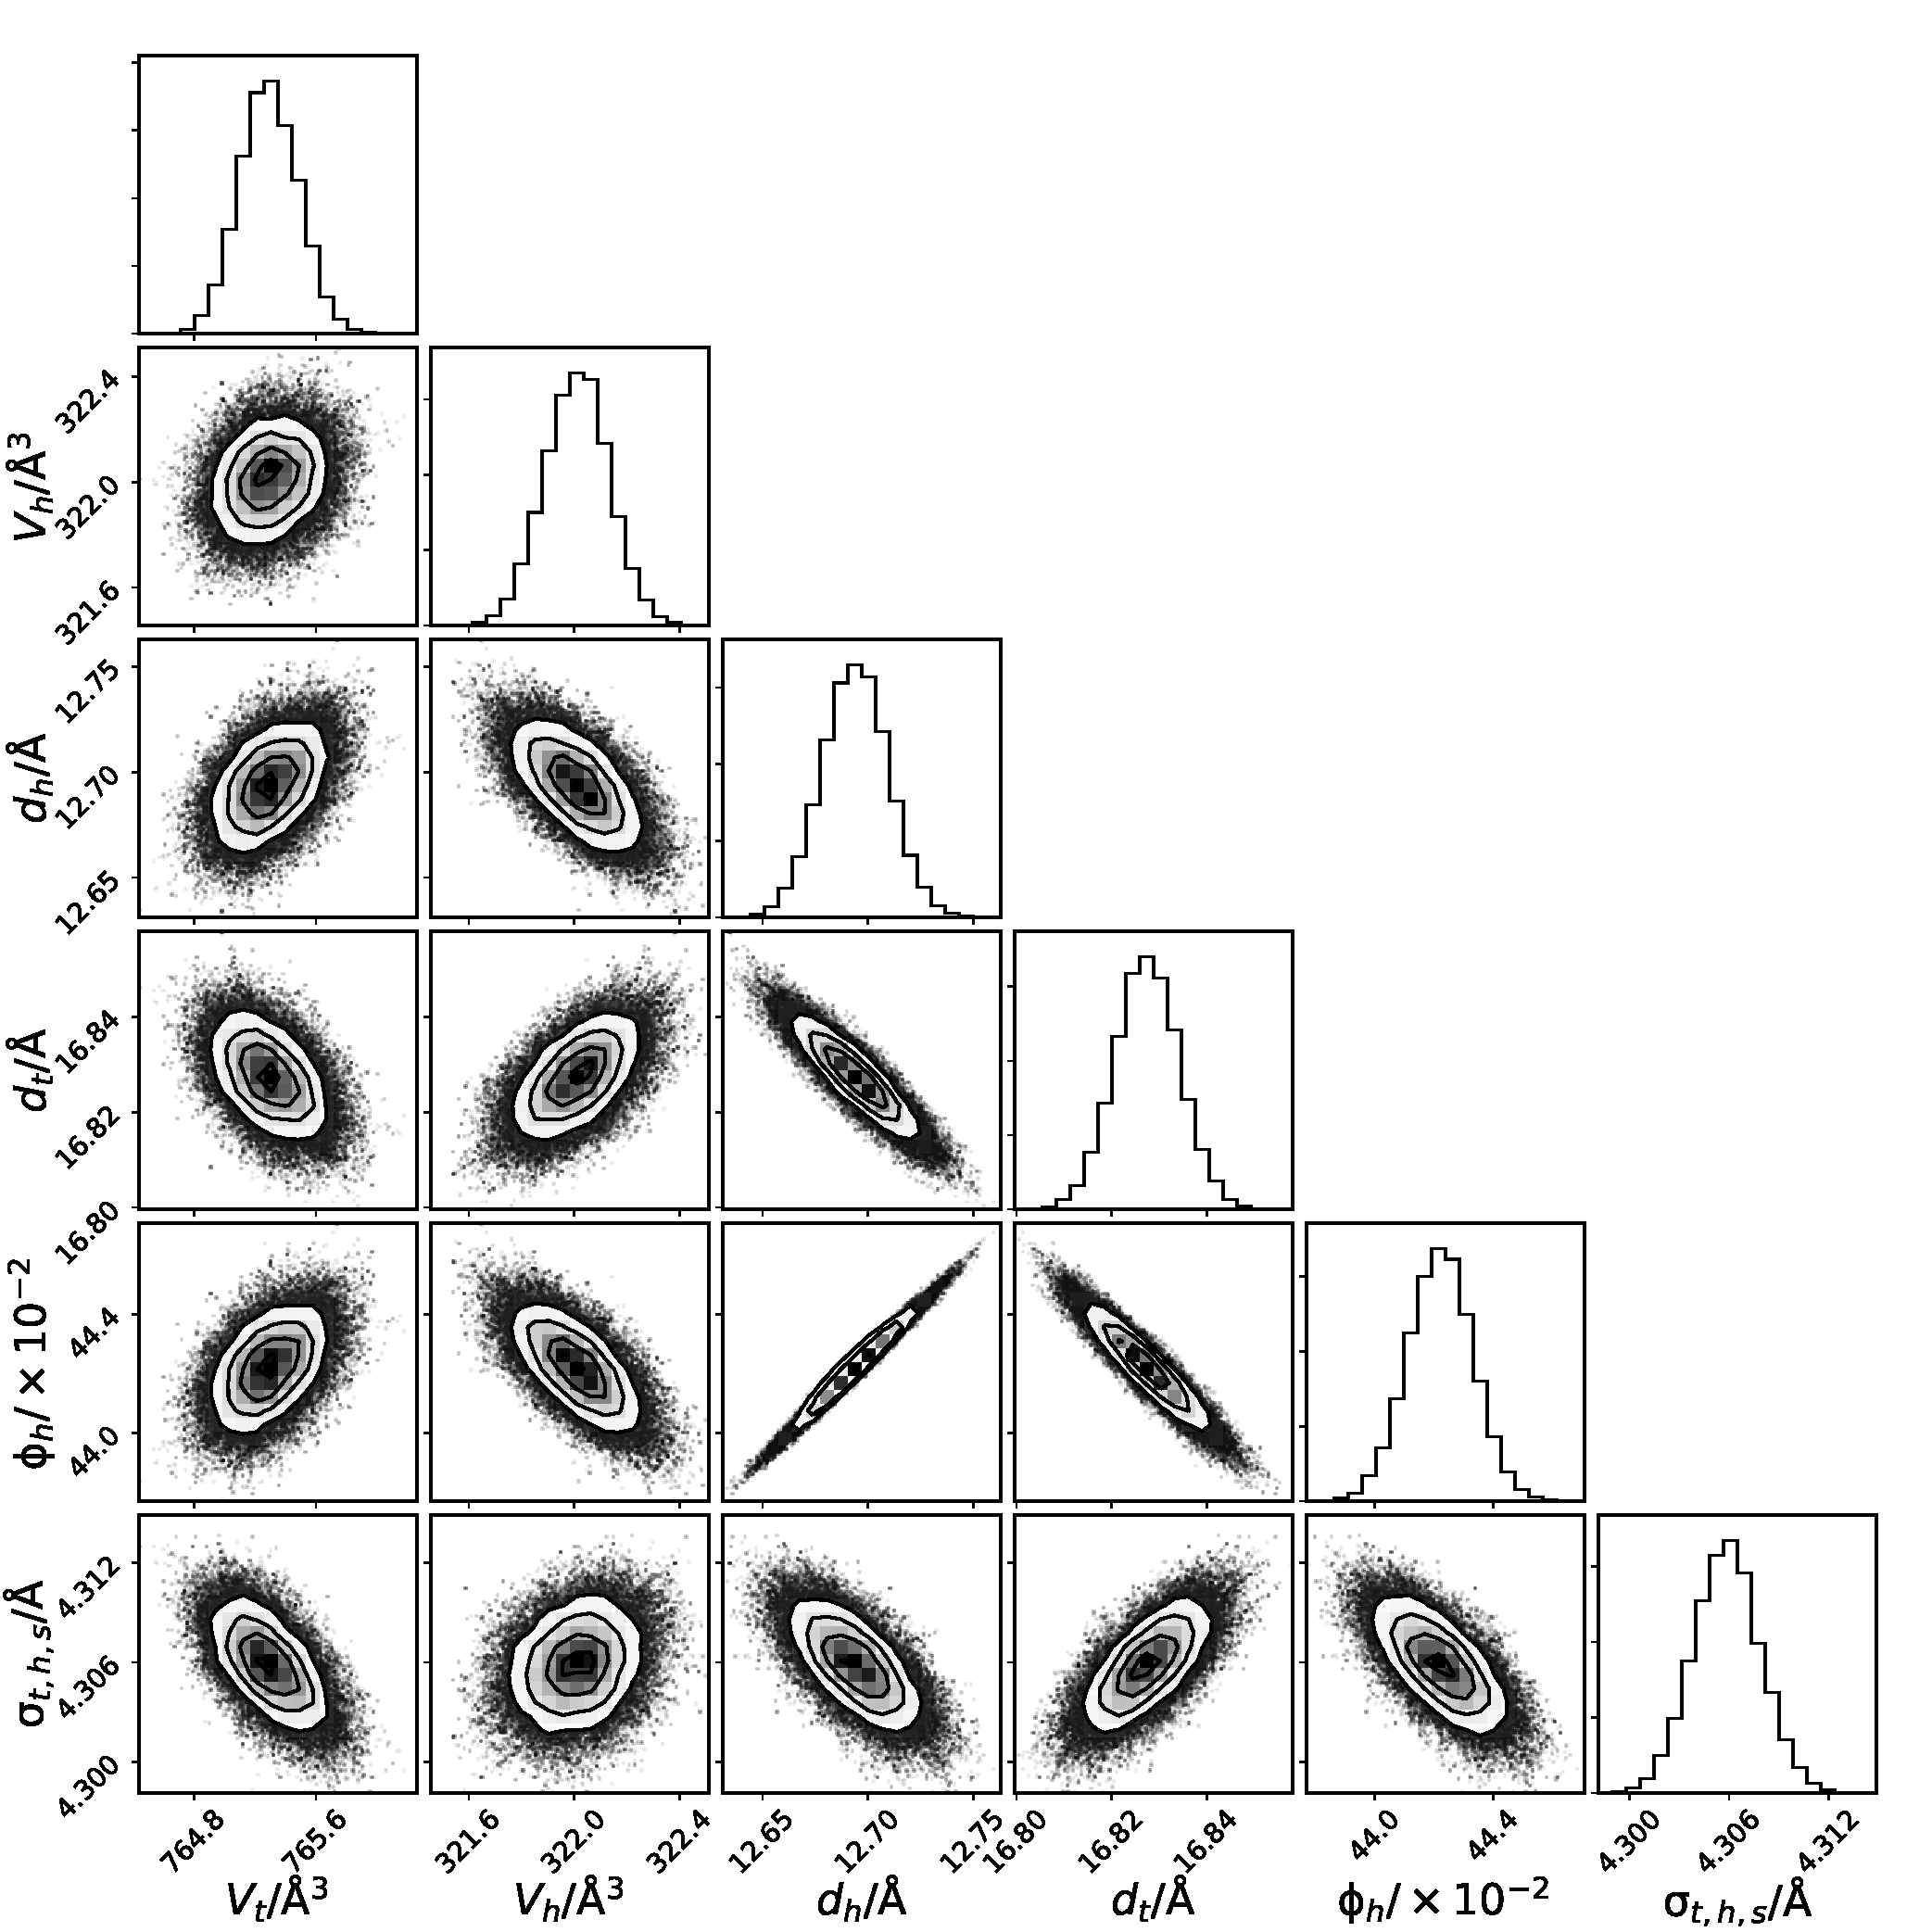
\includegraphics[width=0.50\textwidth]{figures/dppc3_all_corner}
	\caption{The multi-parameter PDFs for the chemically-relevant model of DPPC X-ray reflectometry data at 20 mNm$^{-1}$. Source: Datasets, figure files and running/plotting scripts are available under CC-BY.\cite{mccluskey_2018}}
	\label{fig:dppc3}
\end{figure}
\begin{figure}[h]
	\centering
	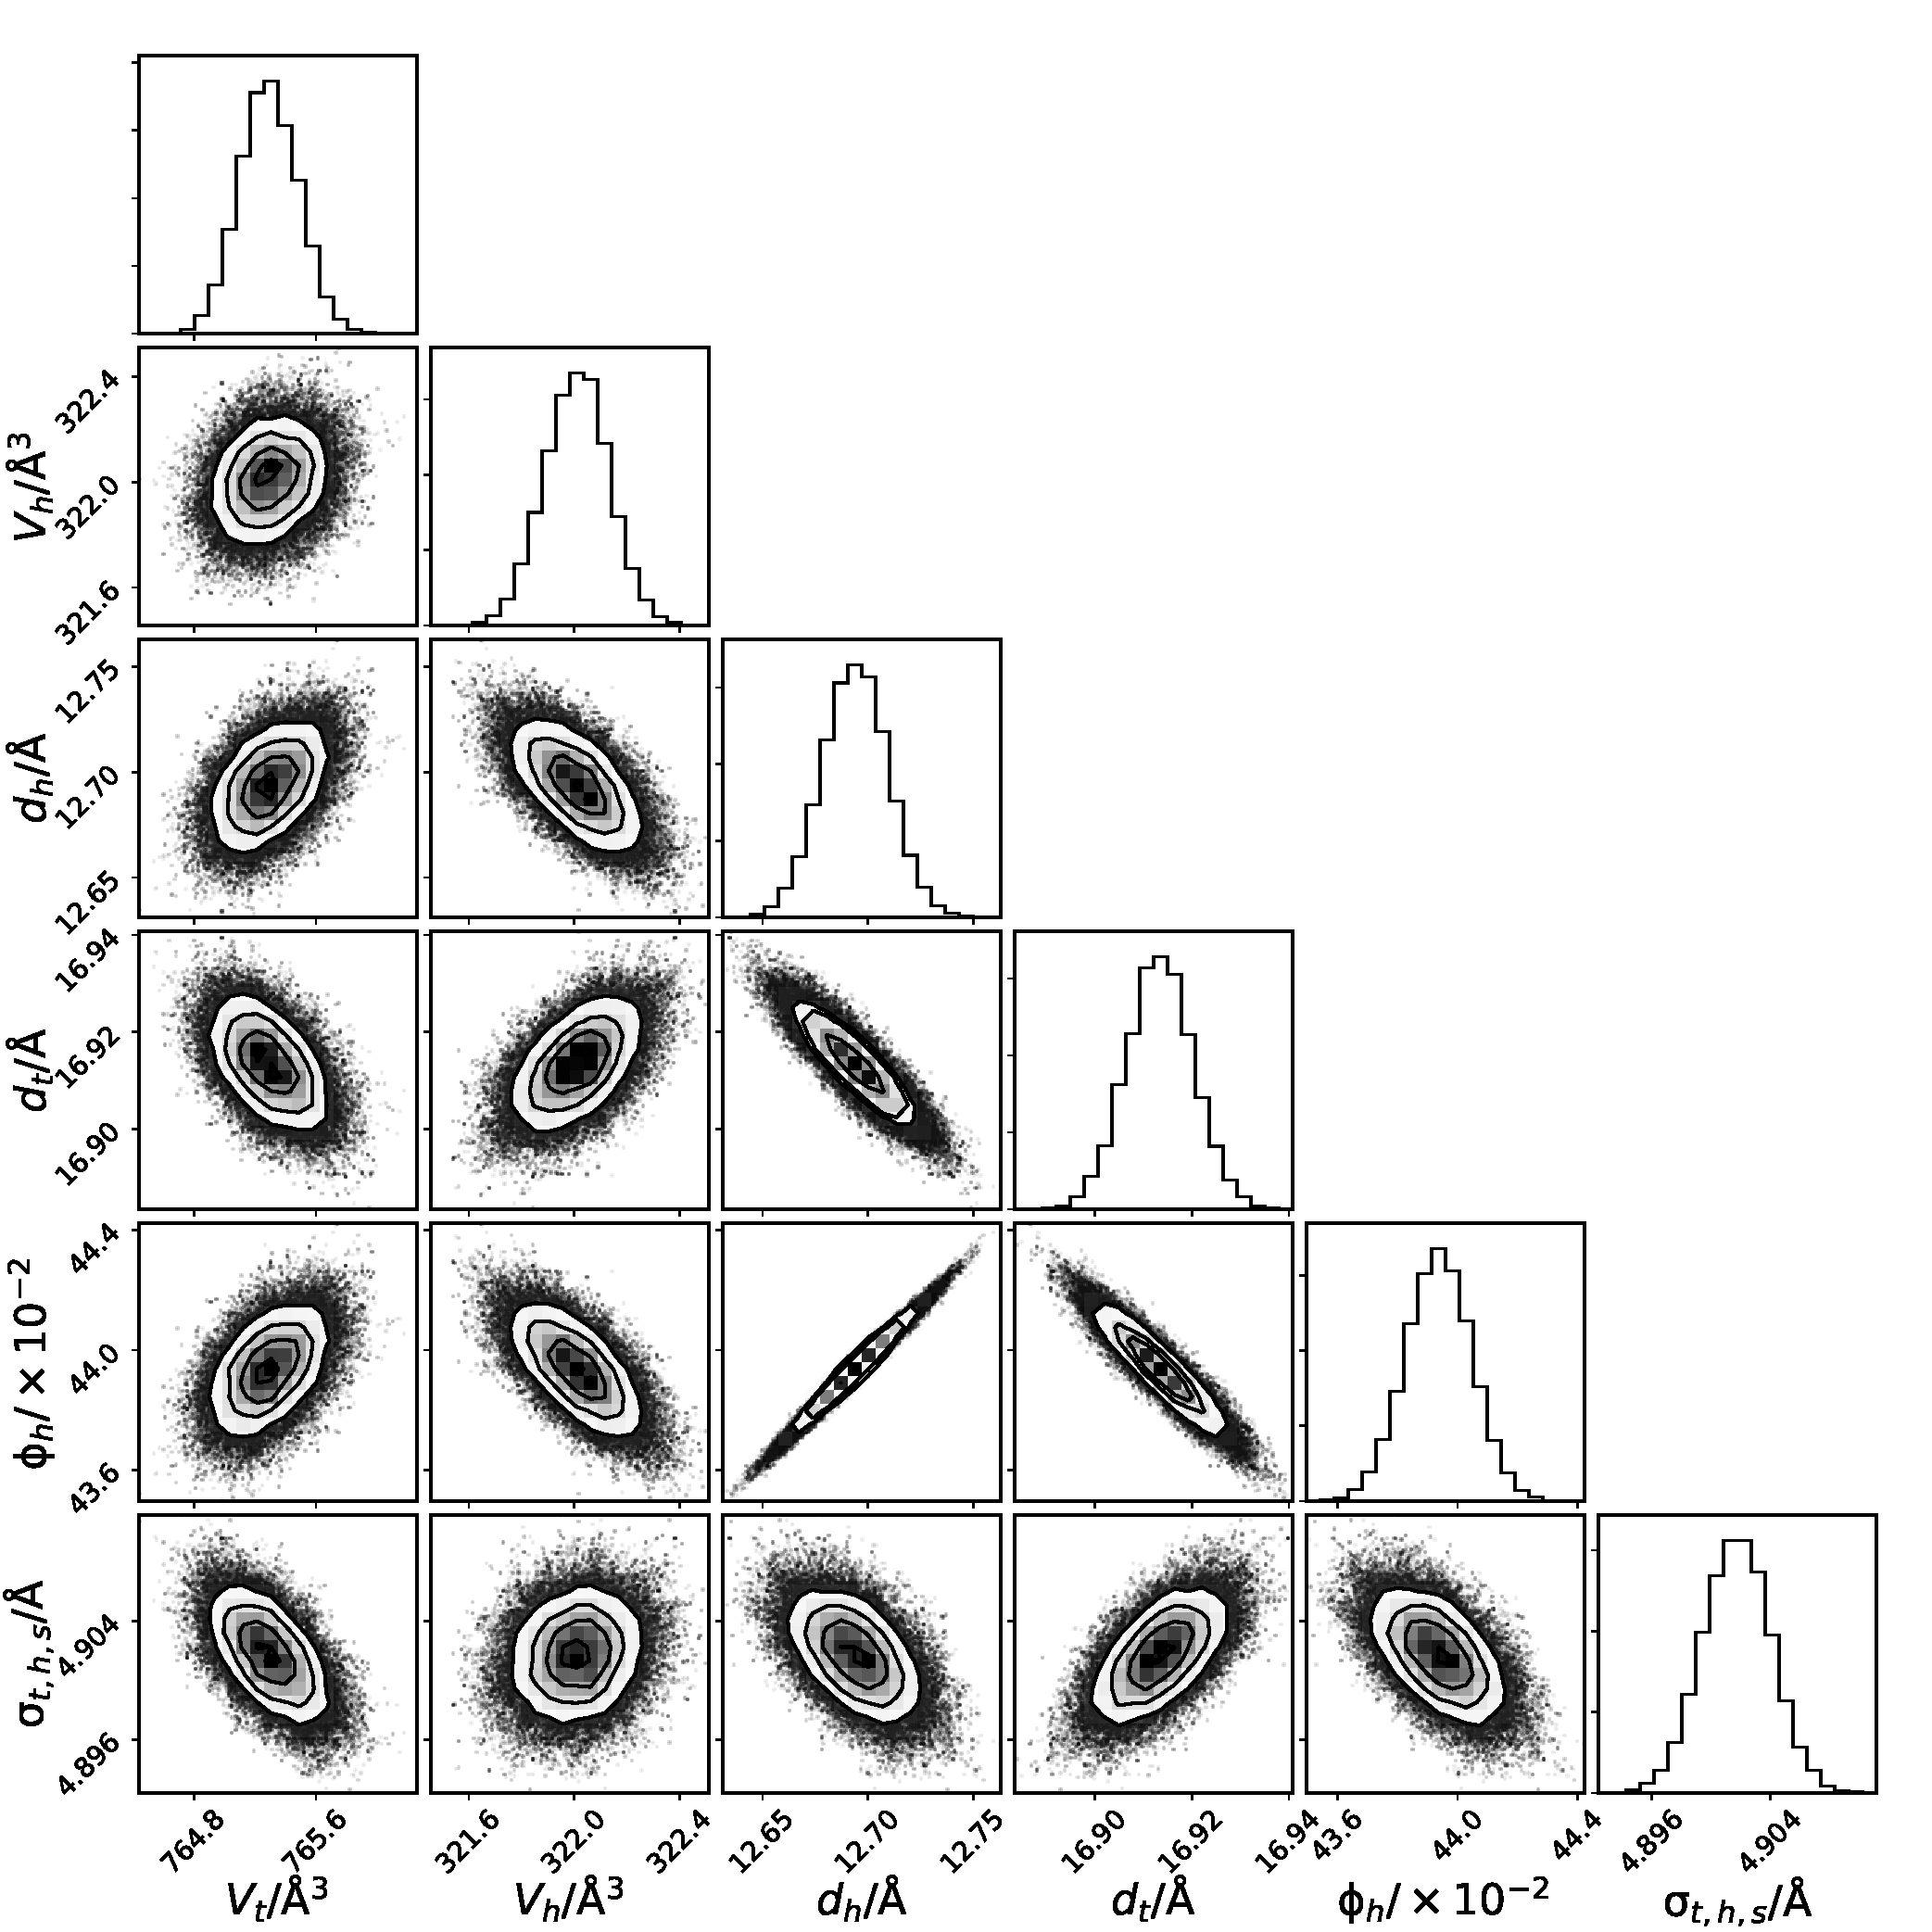
\includegraphics[width=0.50\textwidth]{figures/dppc4_all_corner}
	\caption{The multi-parameter PDFs for the chemically-relevant model of DPPC X-ray reflectometry data at 25 mNm$^{-1}$. Source: Datasets, figure files and running/plotting scripts are available under CC-BY.\cite{mccluskey_2018}}
	\label{fig:dppc4}
\end{figure}
\begin{figure}
	\centering
	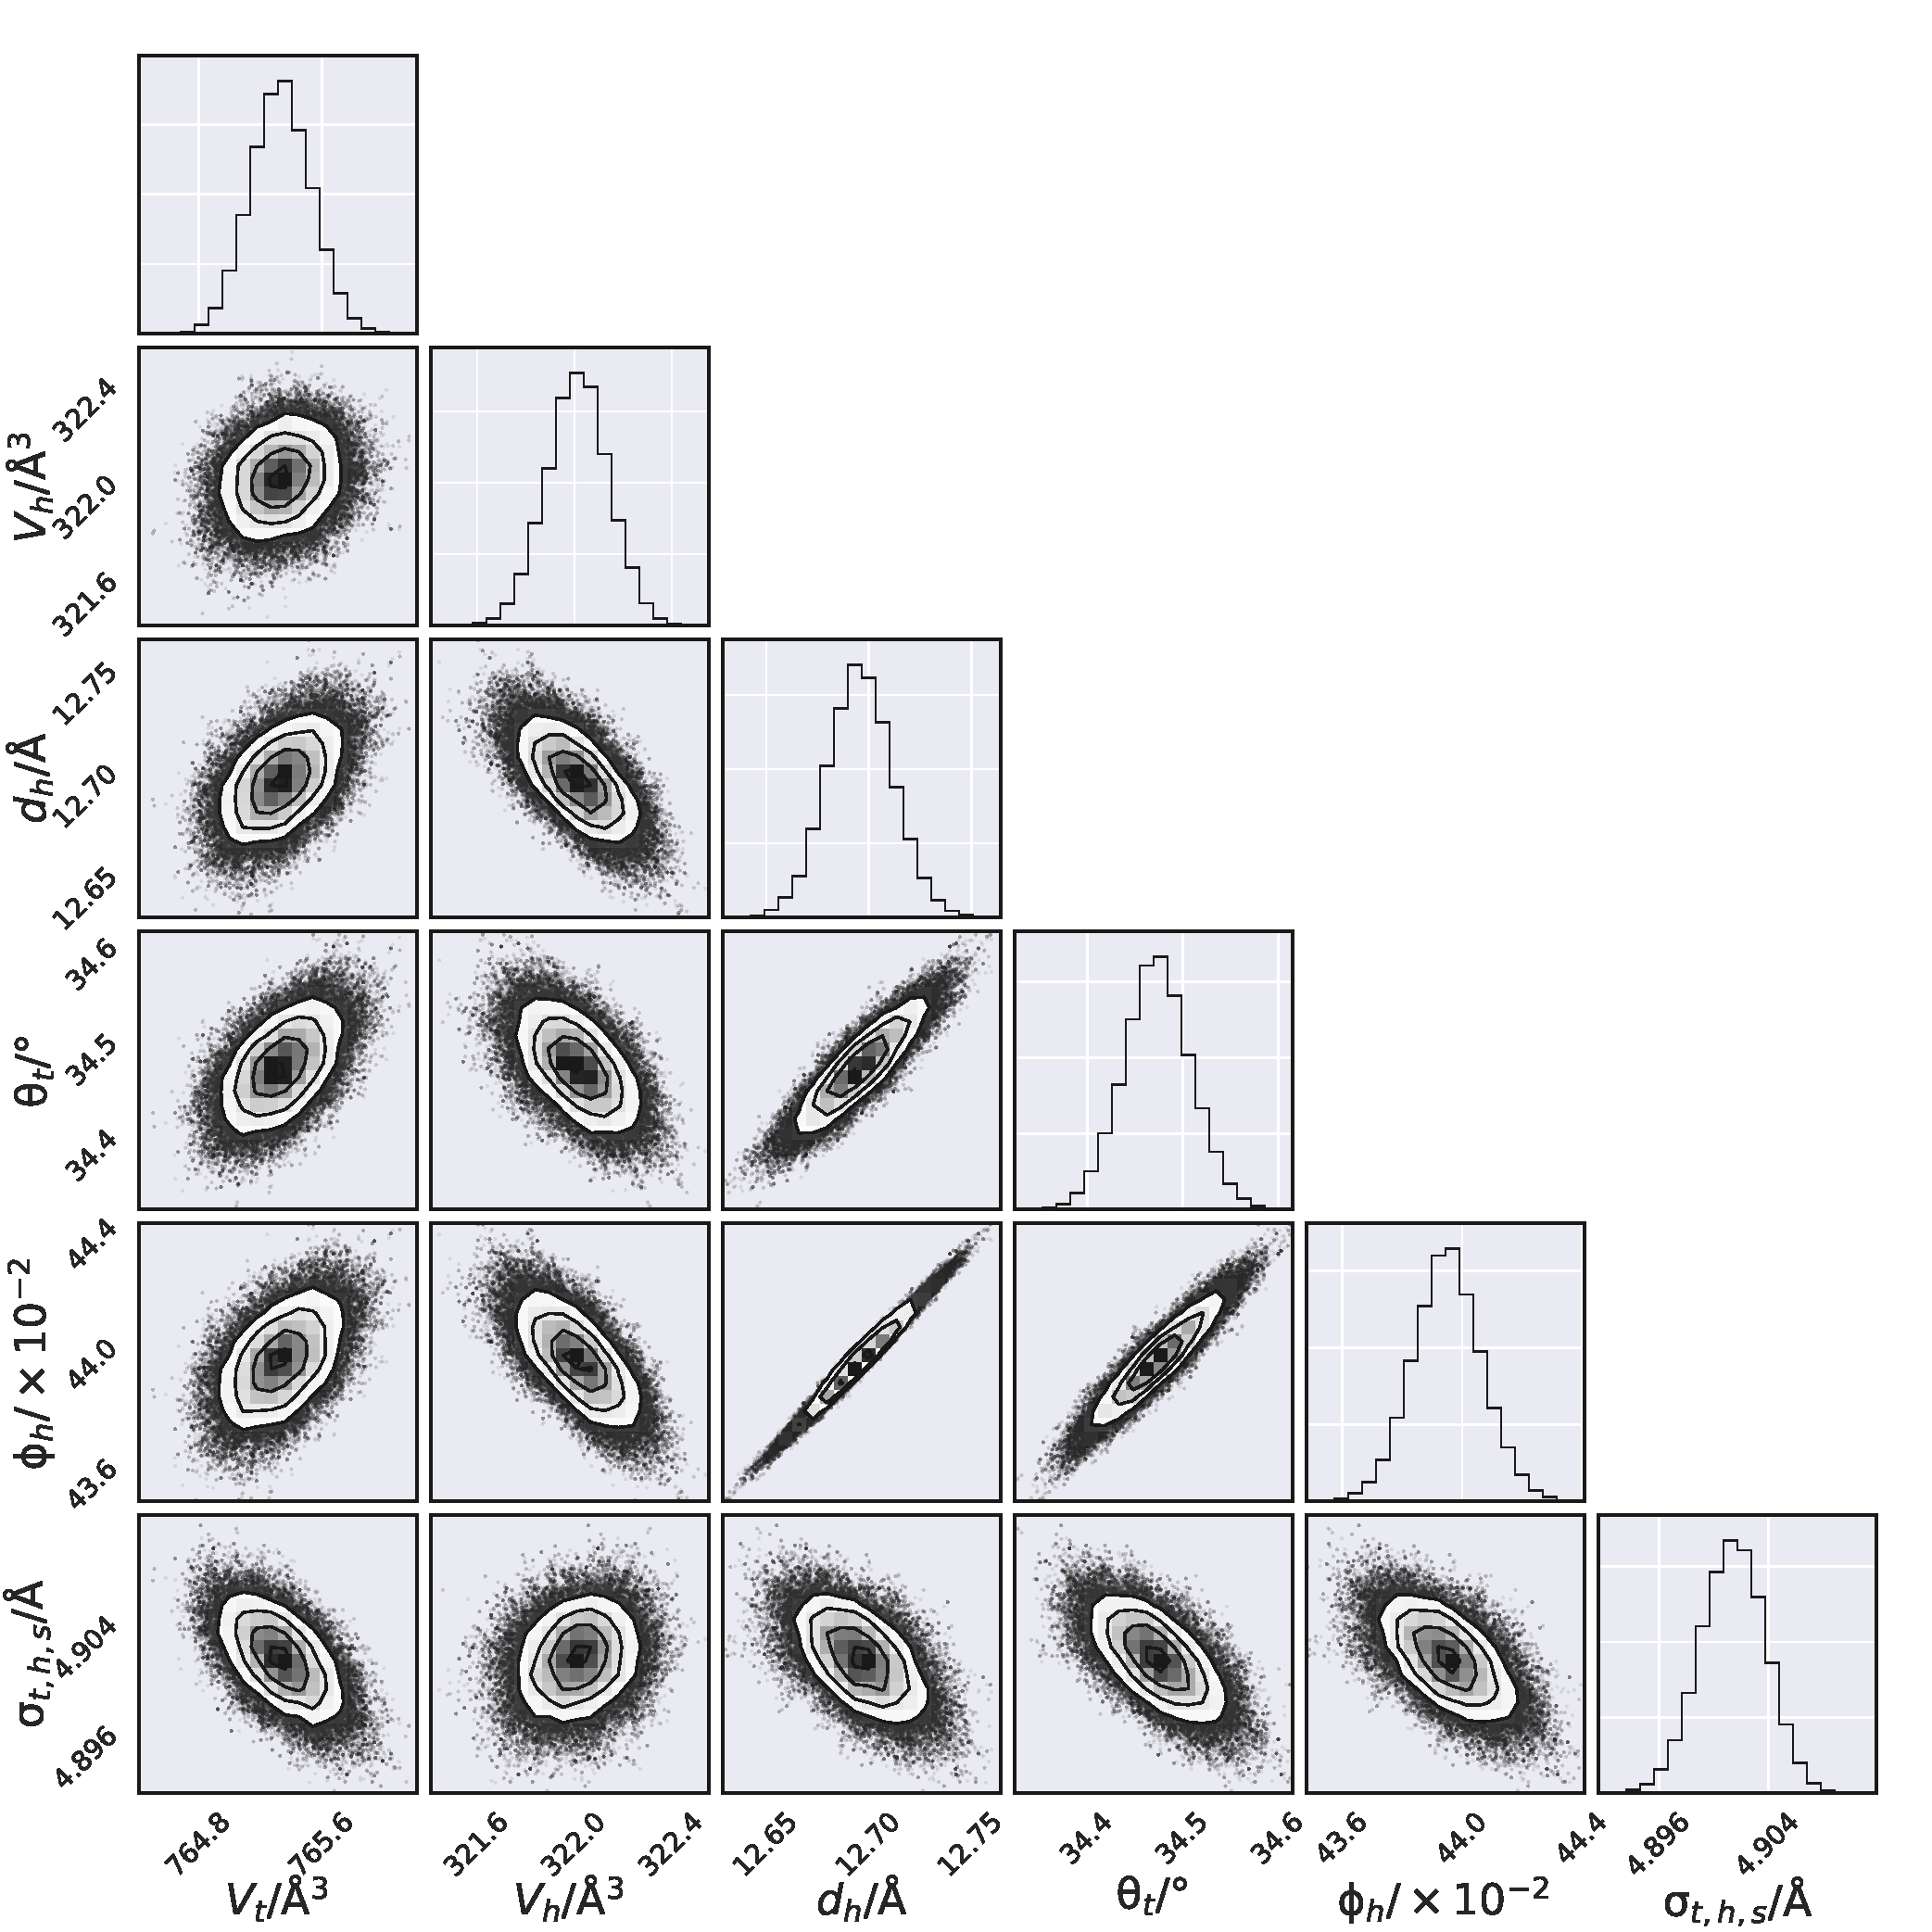
\includegraphics[width=0.50\textwidth]{figures/dppc5_all_corner}
	\caption{The multi-parameter PDFs for the chemically-relevant model of DPPC X-ray reflectometry data at 30 mNm$^{-1}$. Source: Datasets, figure files and running/plotting scripts are available under CC-BY.\cite{mccluskey_2018}}
	\label{fig:dppc5}
\end{figure}
\begin{figure}[h]
	\centering
	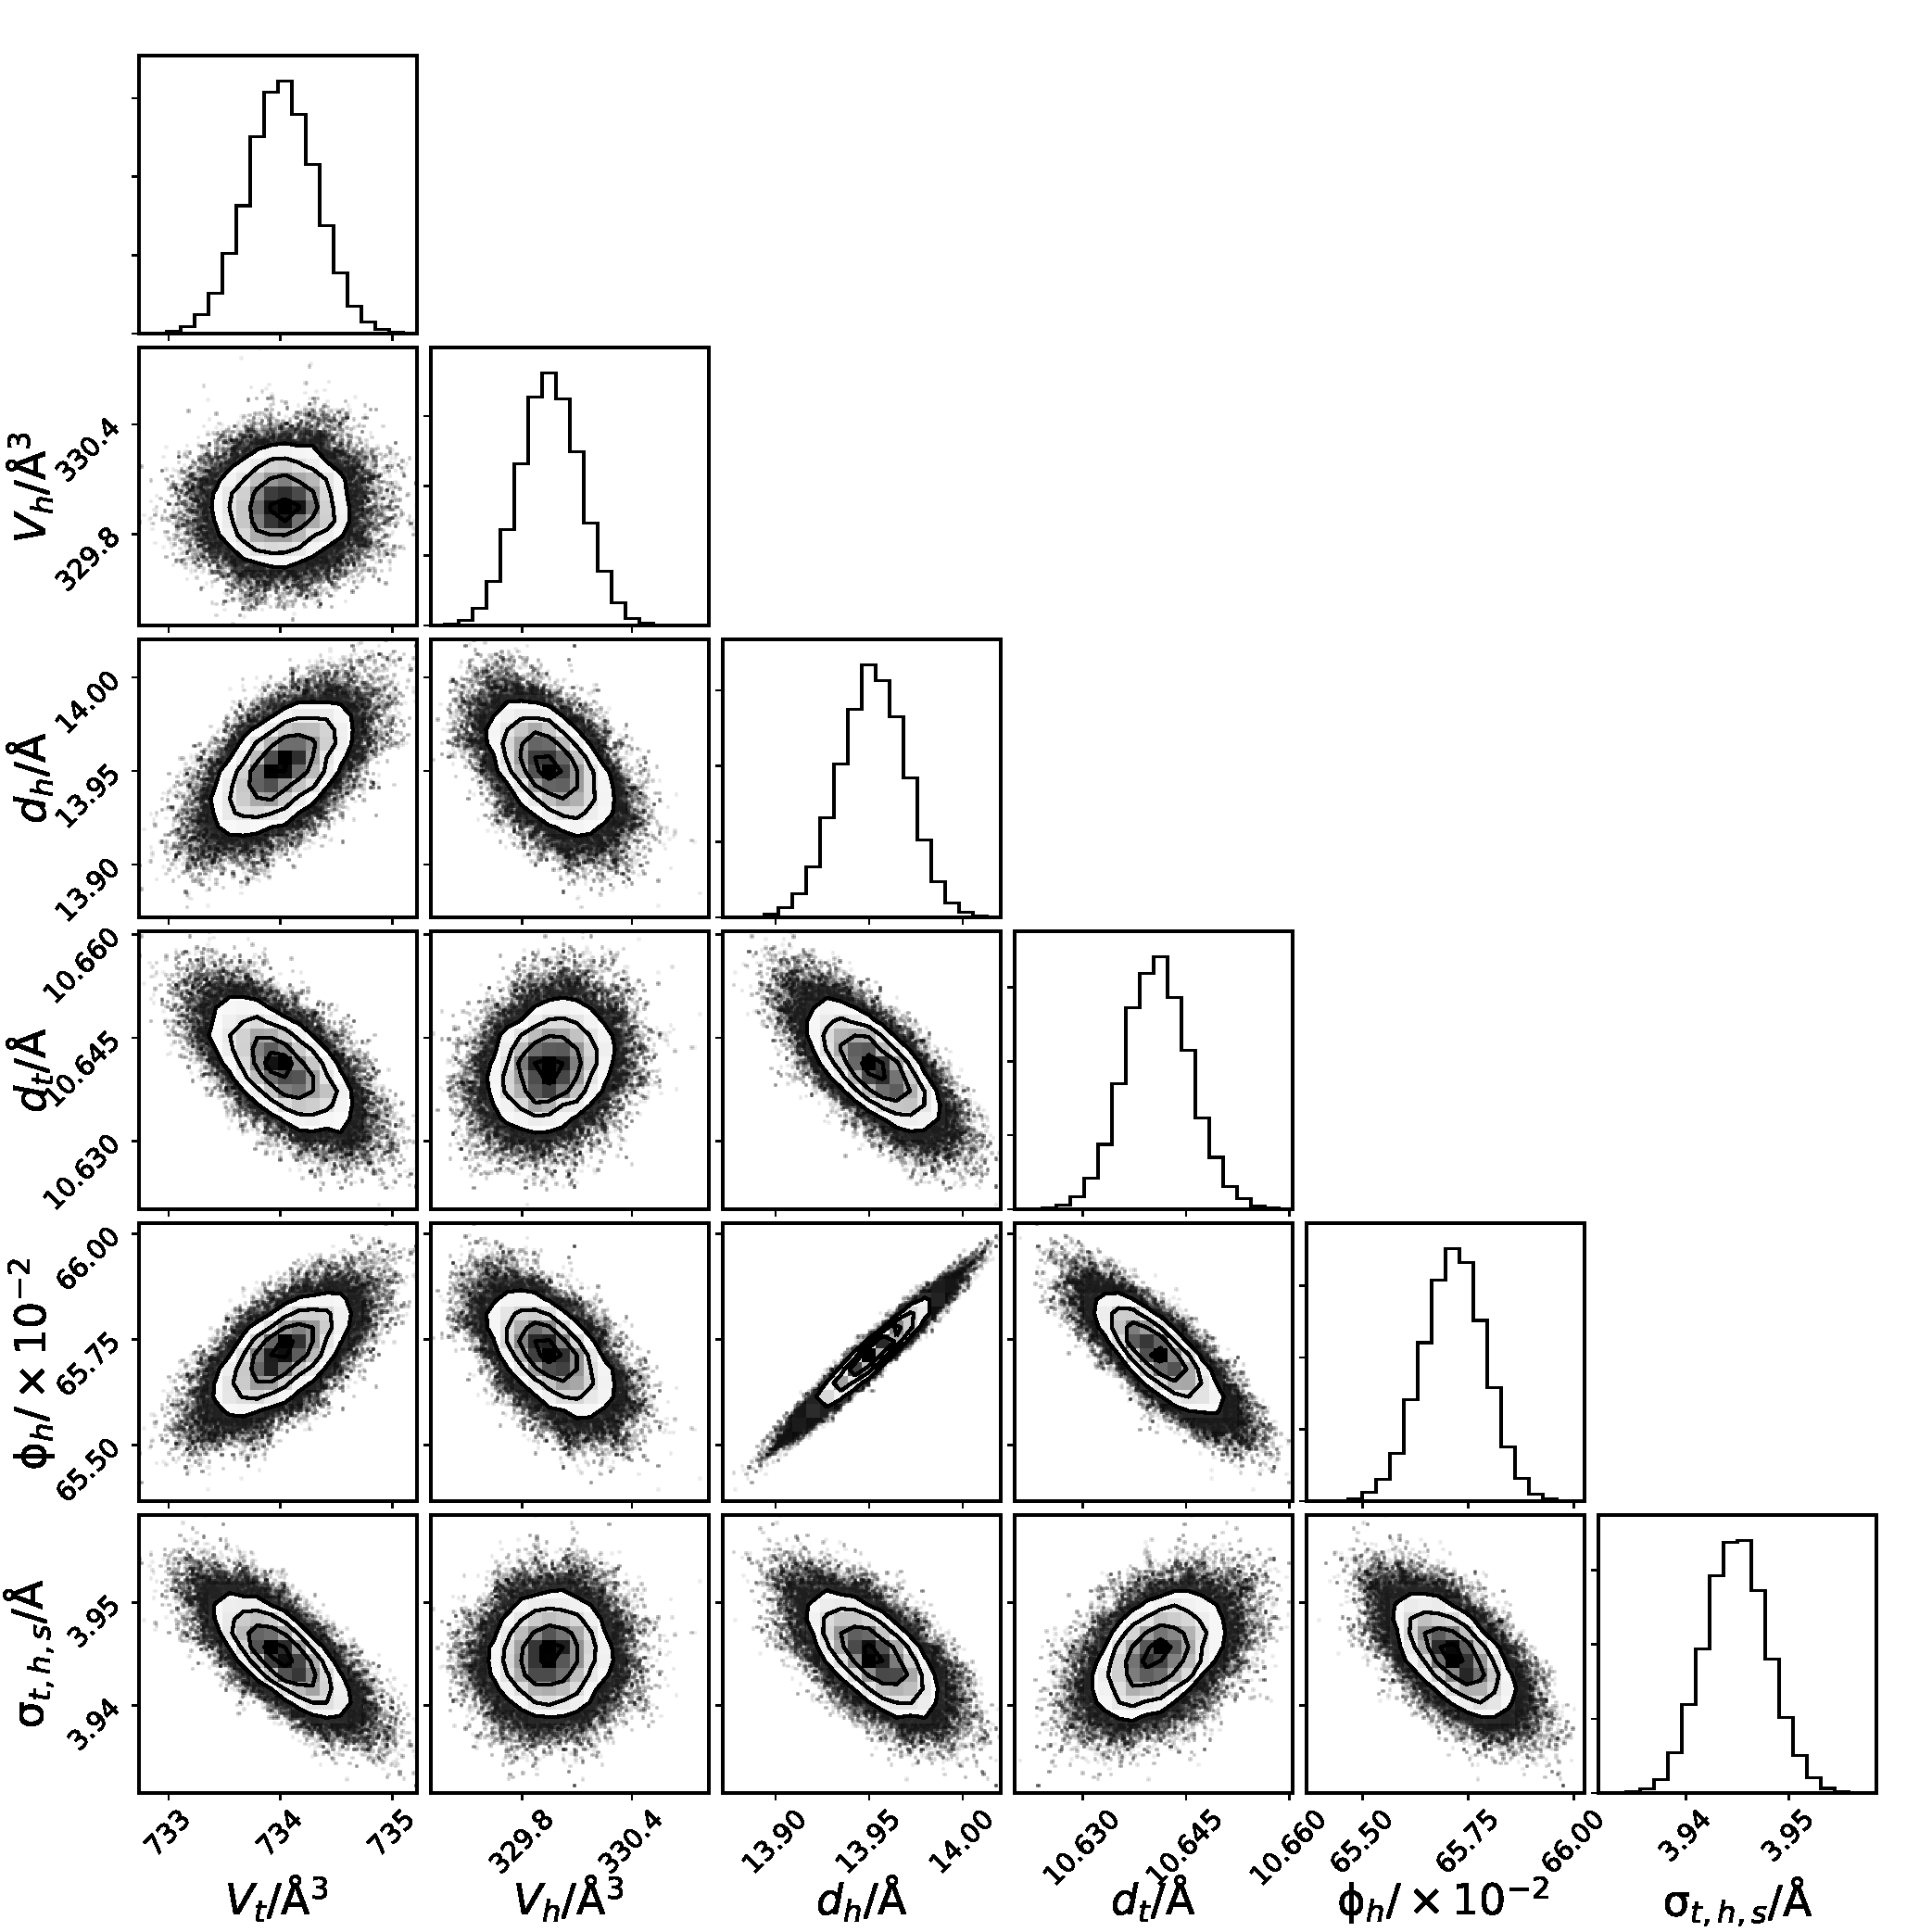
\includegraphics[width=0.50\textwidth]{figures/dmpg2_all_corner}
	\caption{The multi-parameter PDFs for the chemically-relevant model of DMPG X-ray reflectometry data at 15 mNm$^{-1}$. Source: Datasets, figure files and running/plotting scripts are available under CC-BY.\cite{mccluskey_2018}}
	\label{fig:dmpg2}
\end{figure}
\begin{figure}[h]
	\centering
	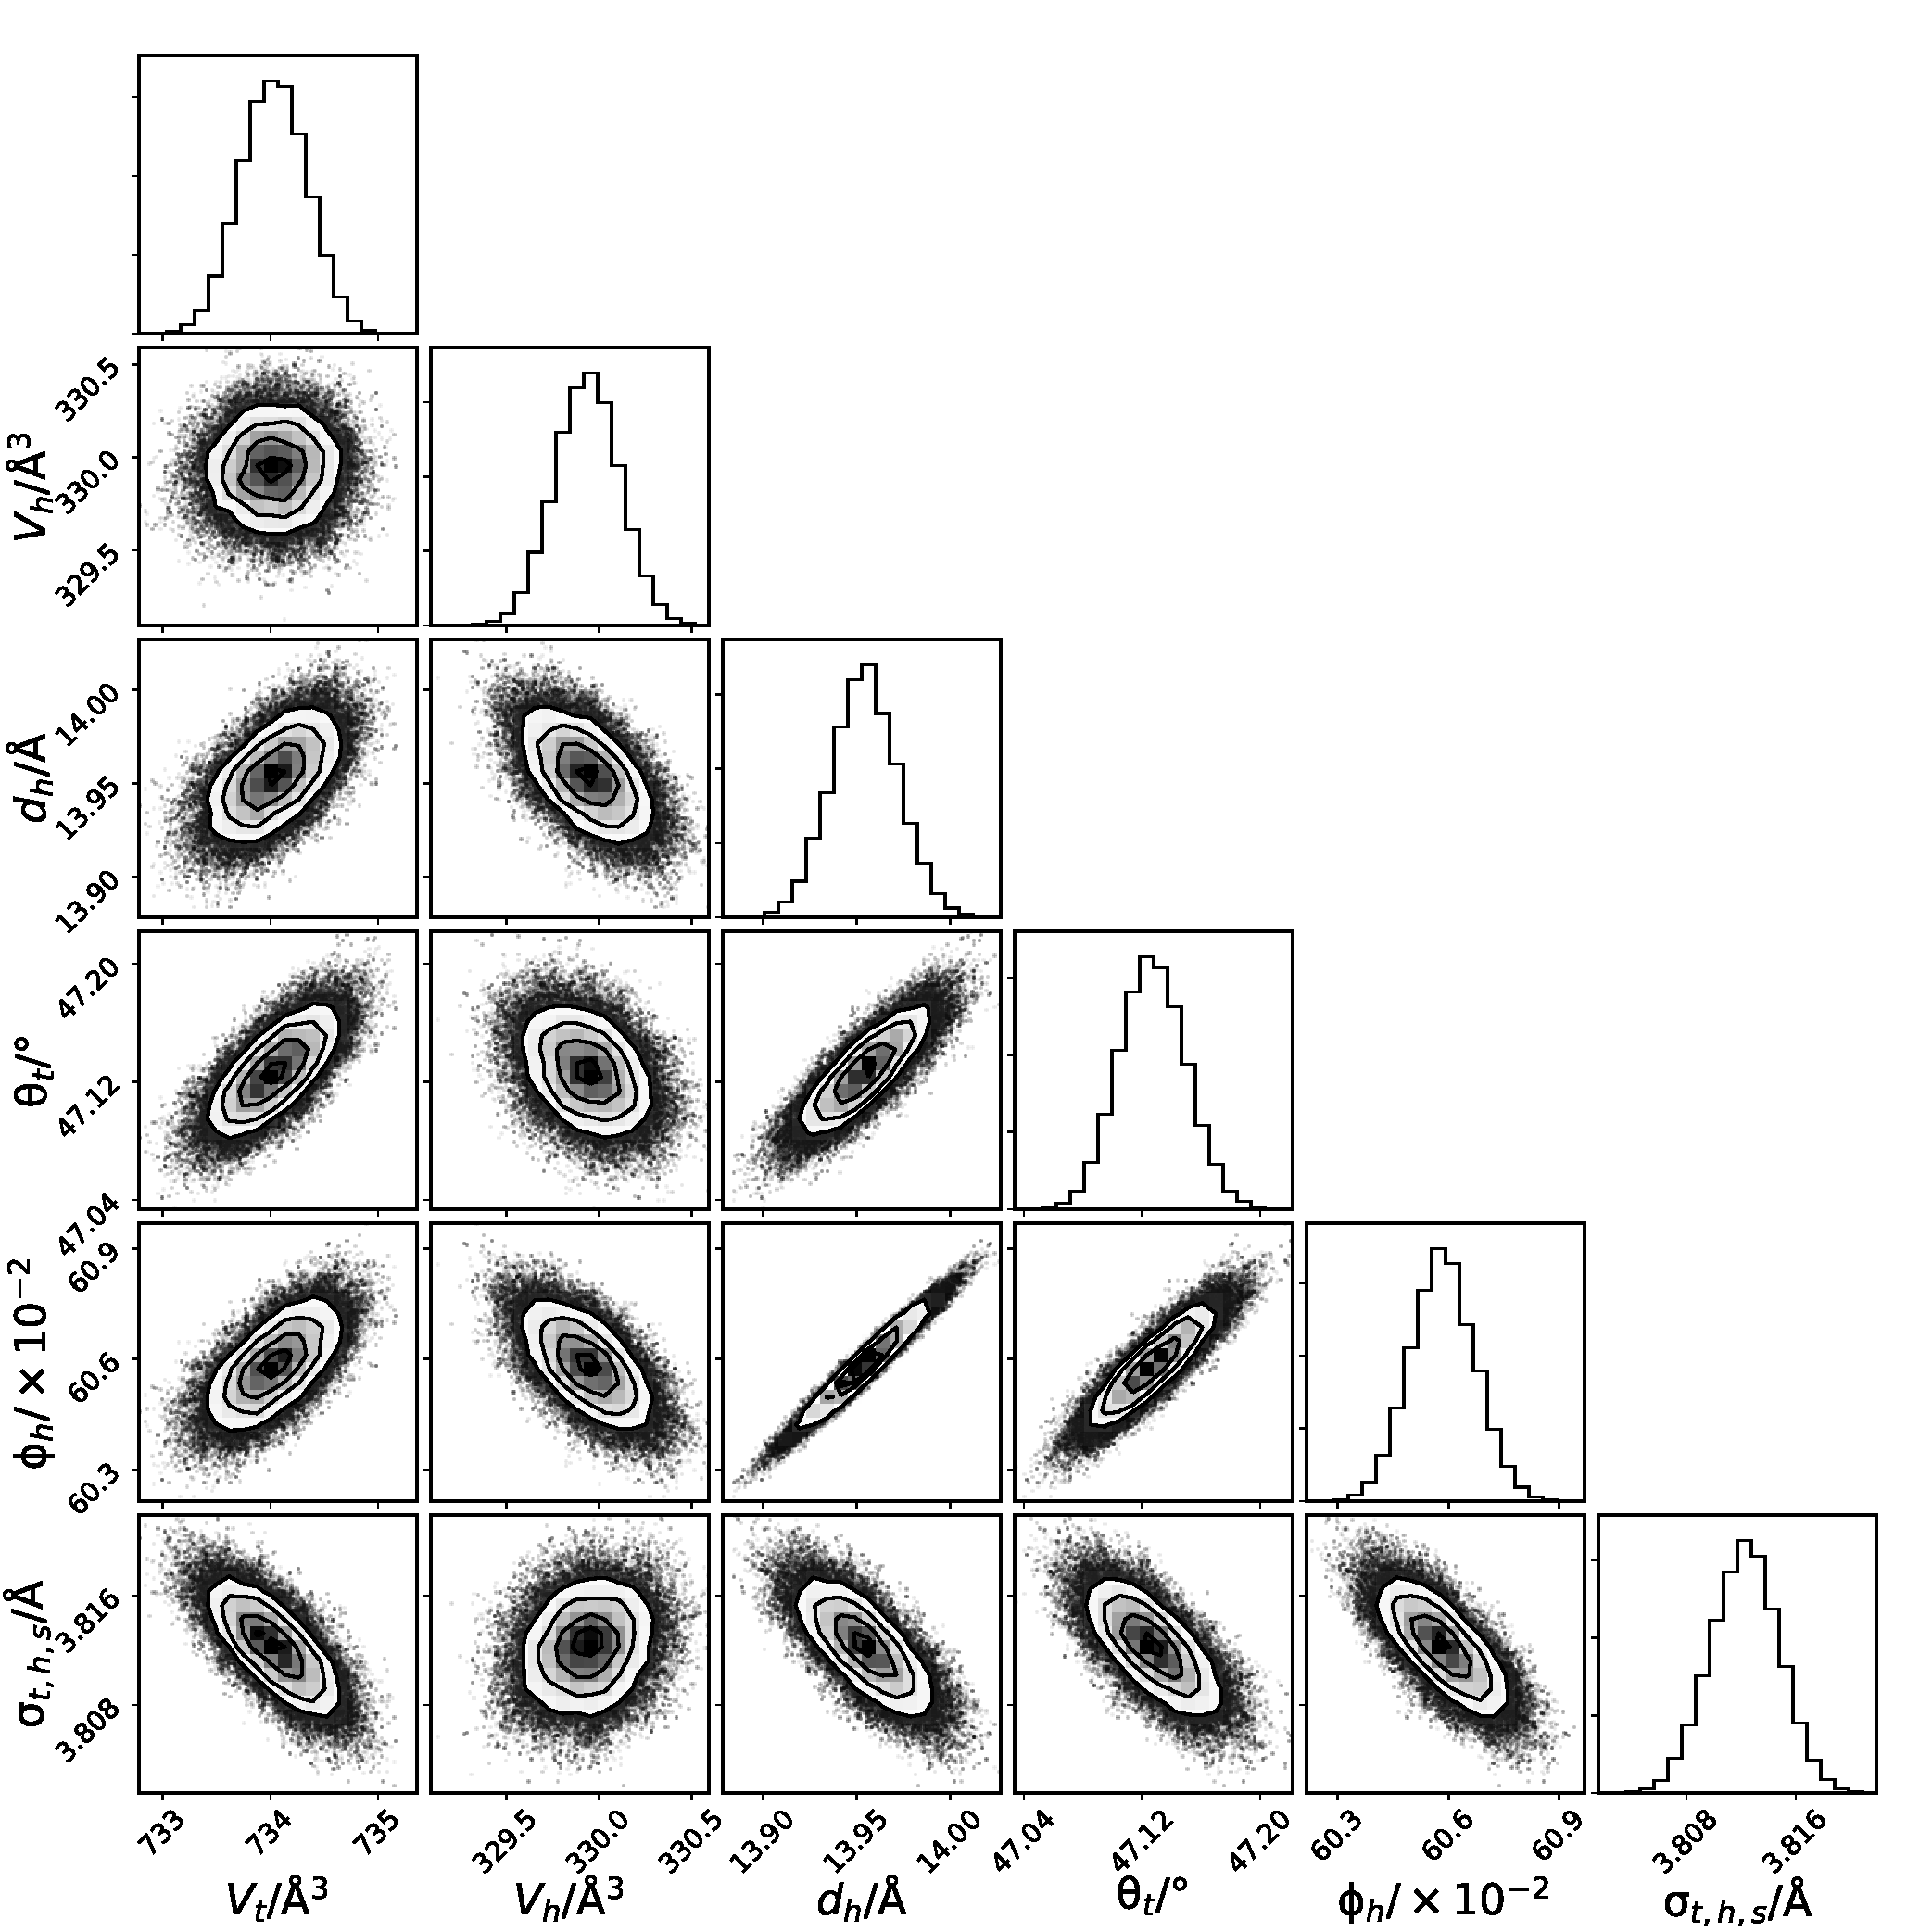
\includegraphics[width=0.50\textwidth]{figures/dmpg3_all_corner}
	\caption{The multi-parameter PDFs for the chemically-relevant model of DMPG X-ray reflectometry data at 20 mNm$^{-1}$. Source: Datasets, figure files and running/plotting scripts are available under CC-BY.\cite{mccluskey_2018}}
	\label{fig:dmpg3}
\end{figure}
\begin{figure}[h]
	\centering
	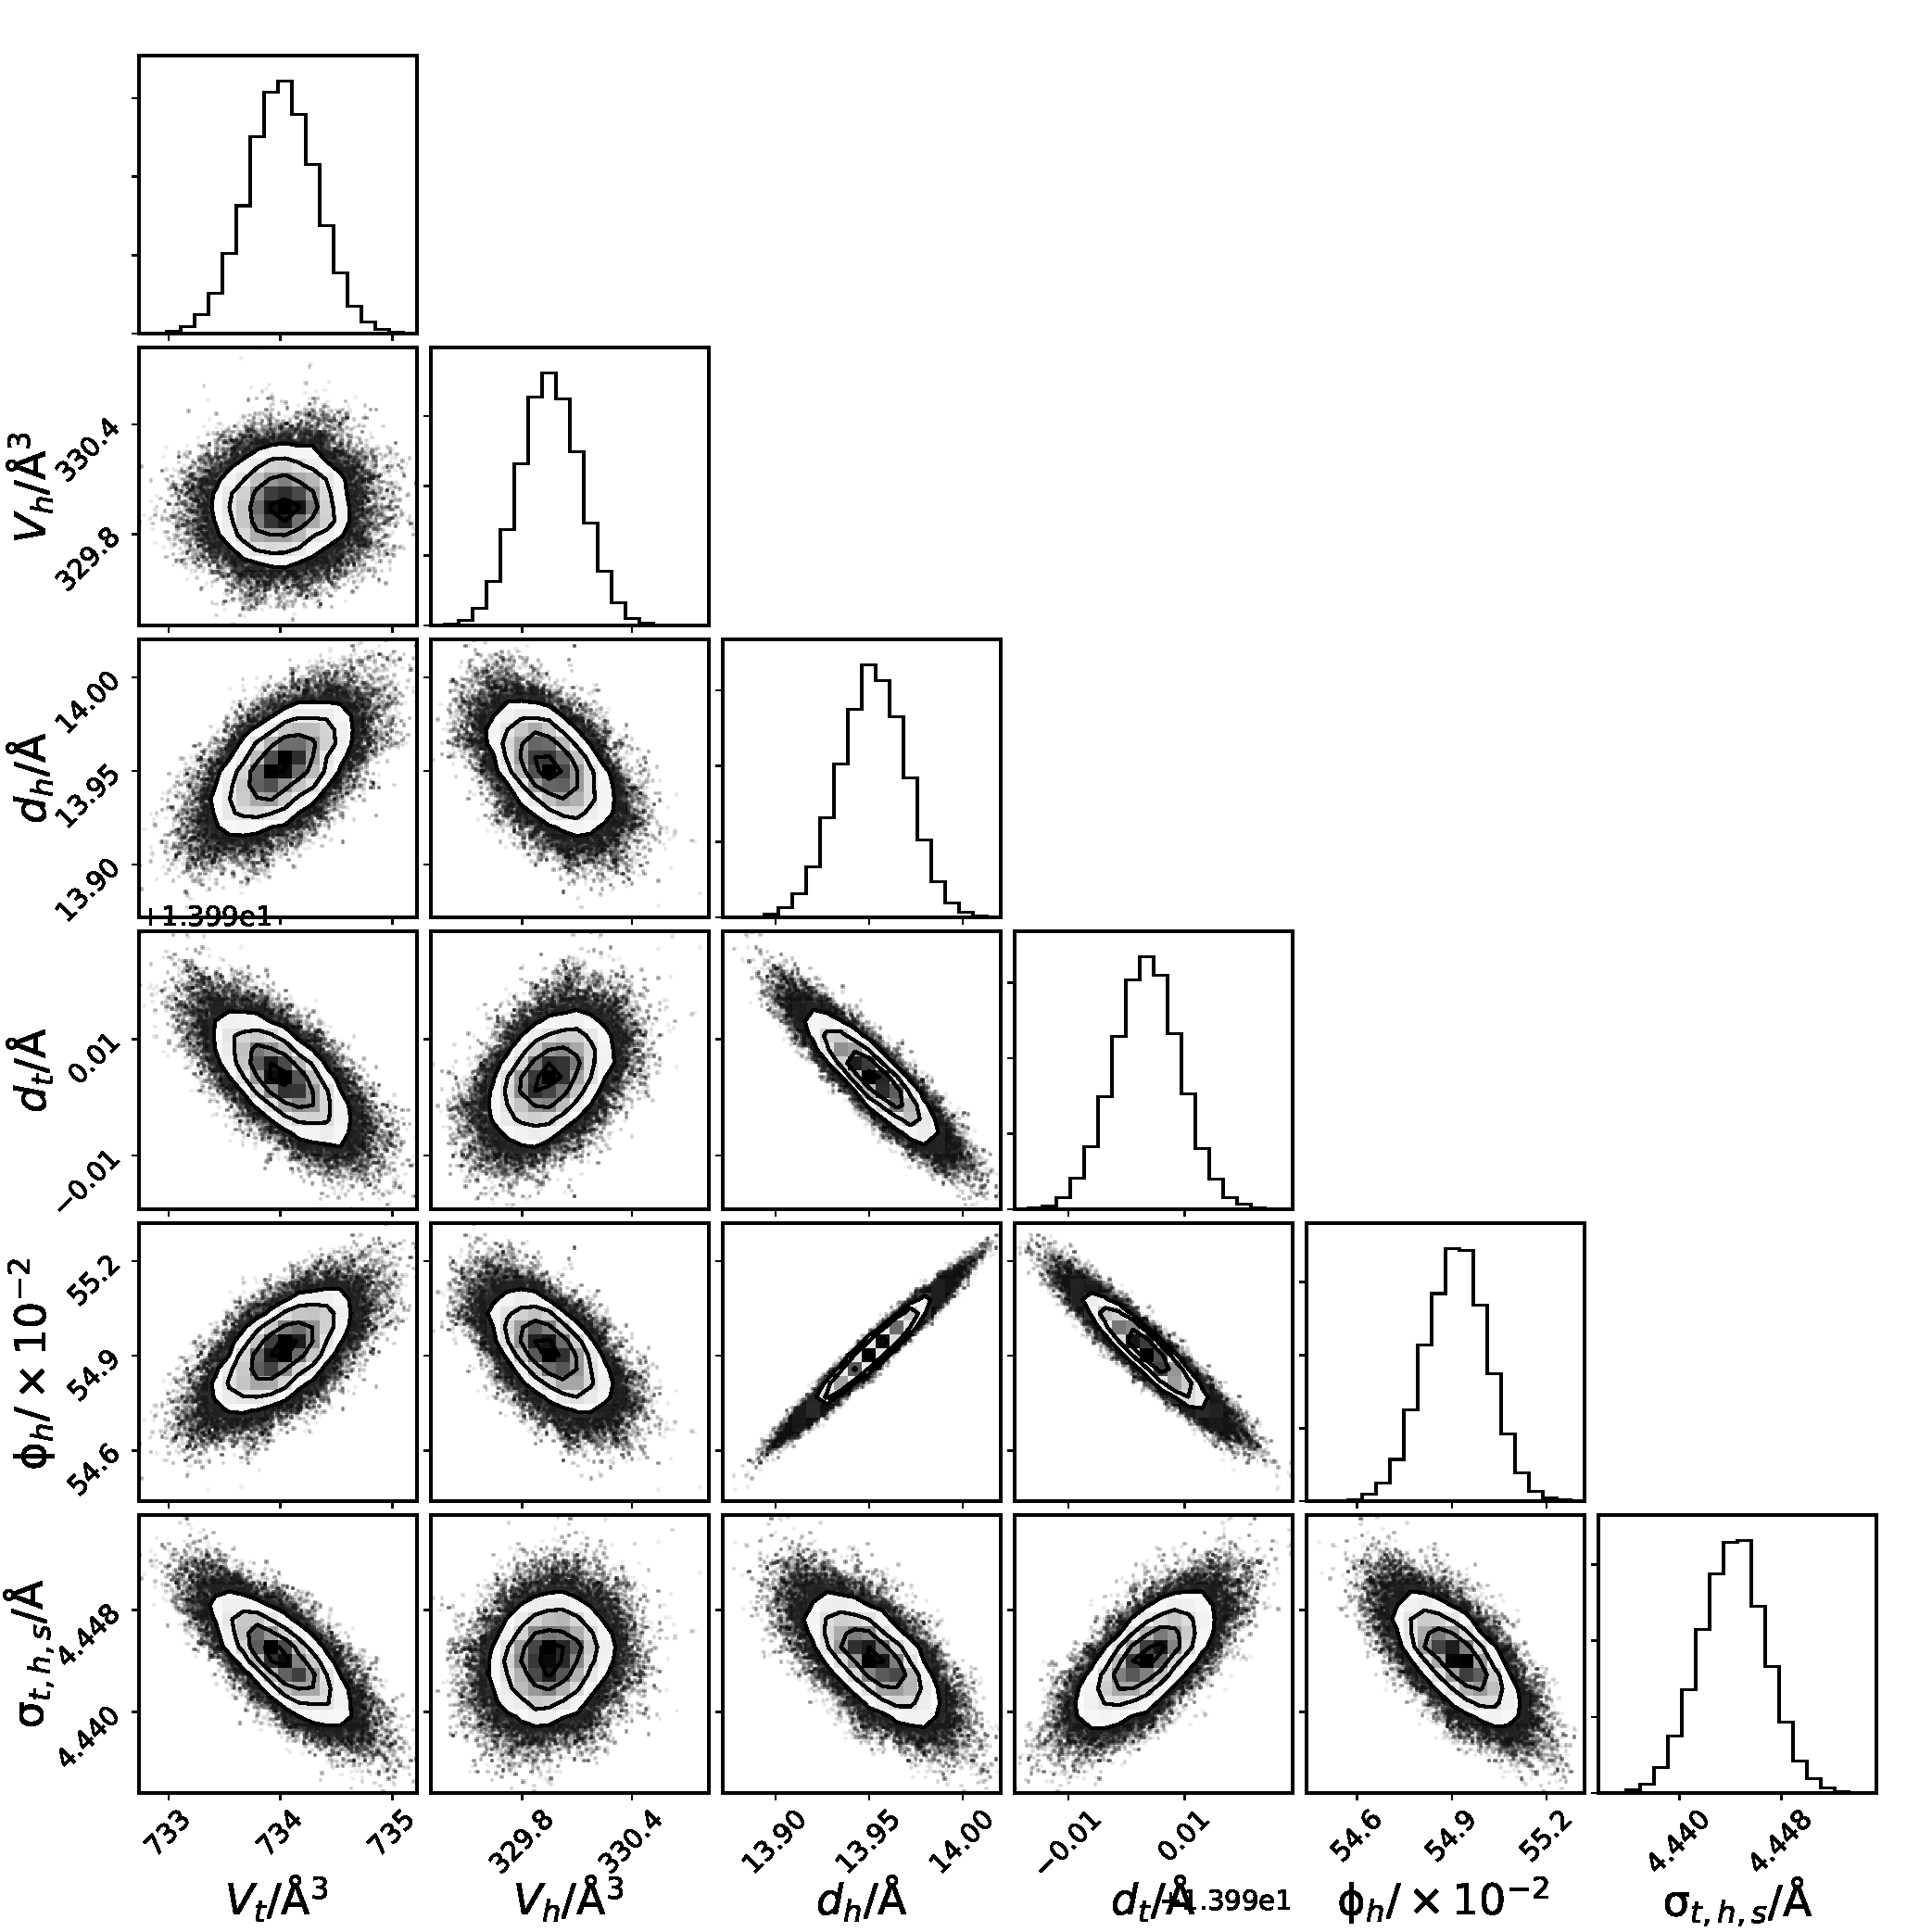
\includegraphics[width=0.50\textwidth]{figures/dmpg4_all_corner}
	\caption{The multi-parameter PDFs for the chemically-relevant model of DMPG X-ray reflectometry data at 25 mNm$^{-1}$. Source: Datasets, figure files and running/plotting scripts are available under CC-BY.\cite{mccluskey_2018}}
	\label{fig:dmpg4}
\end{figure}
\begin{figure}
	\centering
	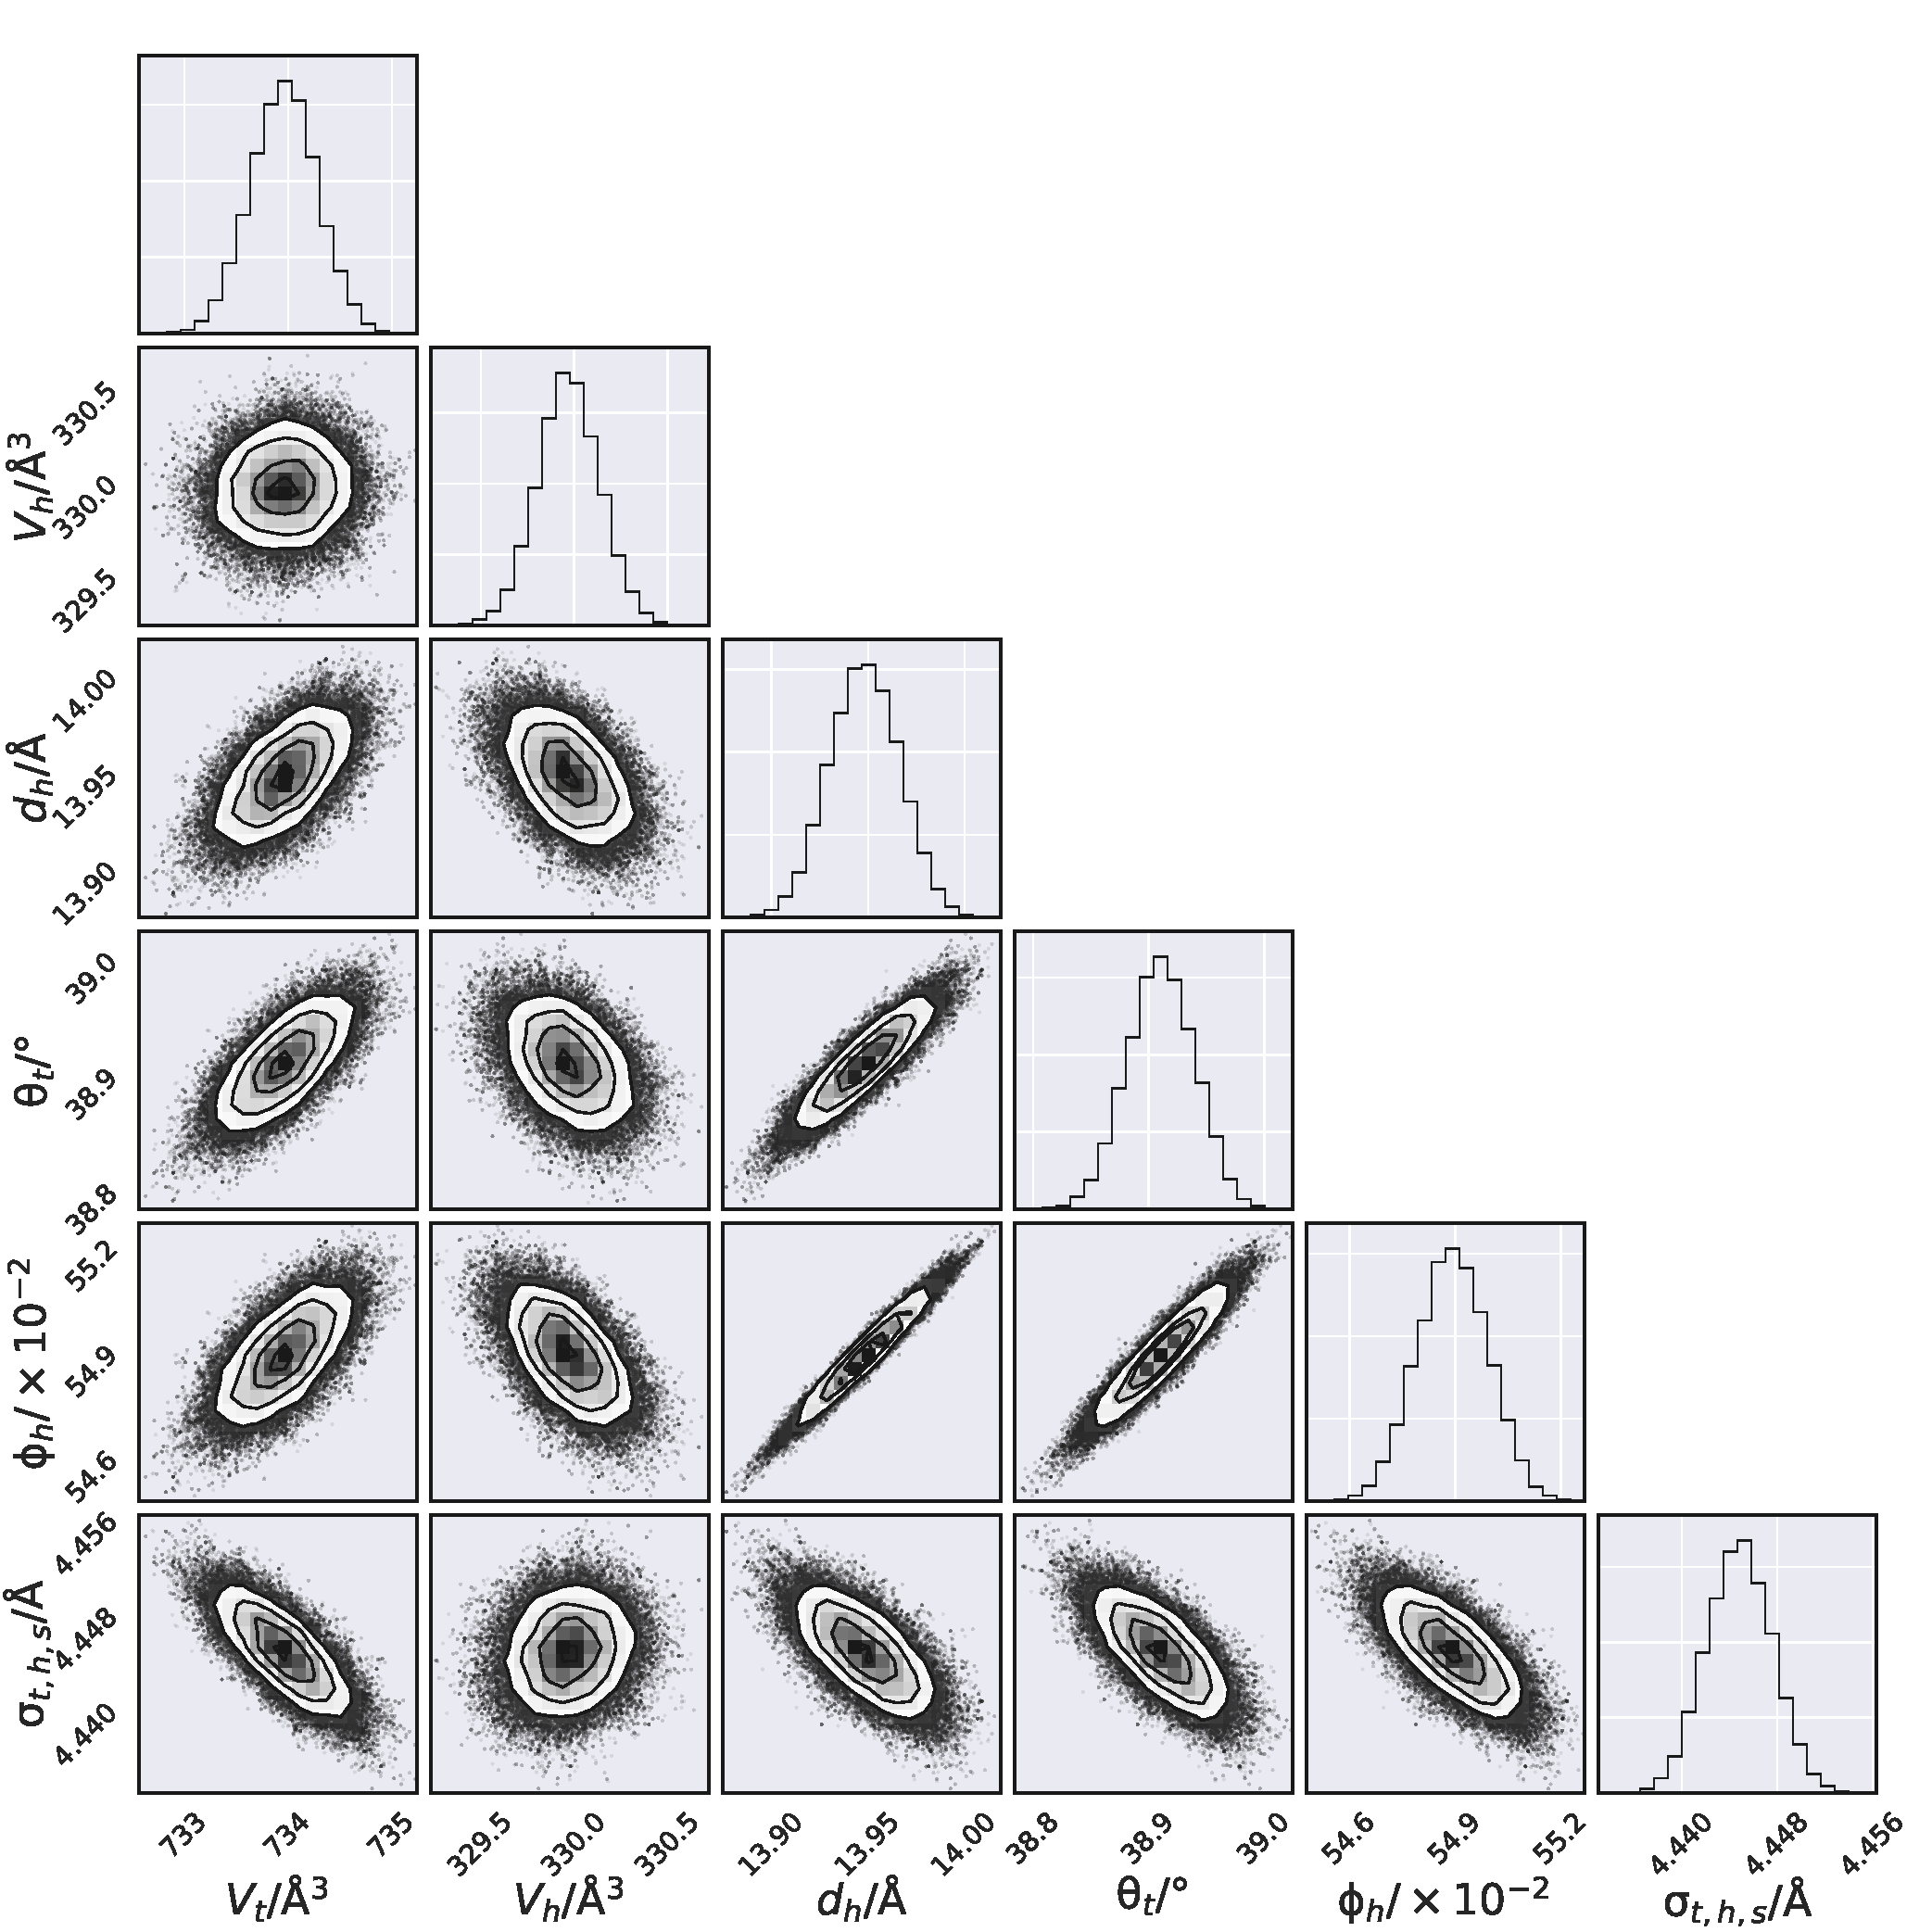
\includegraphics[width=0.50\textwidth]{figures/dmpg5_all_corner}
	\caption{The multi-parameter PDFs for the chemically-relevant model of DMPG X-ray reflectometry data at 30 mNm$^{-1}$. Source: Datasets, figure files and running/plotting scripts are available under CC-BY.\cite{mccluskey_2018}}
	\label{fig:dmpg5}
\end{figure}
\begin{figure}[h]
	\centering
	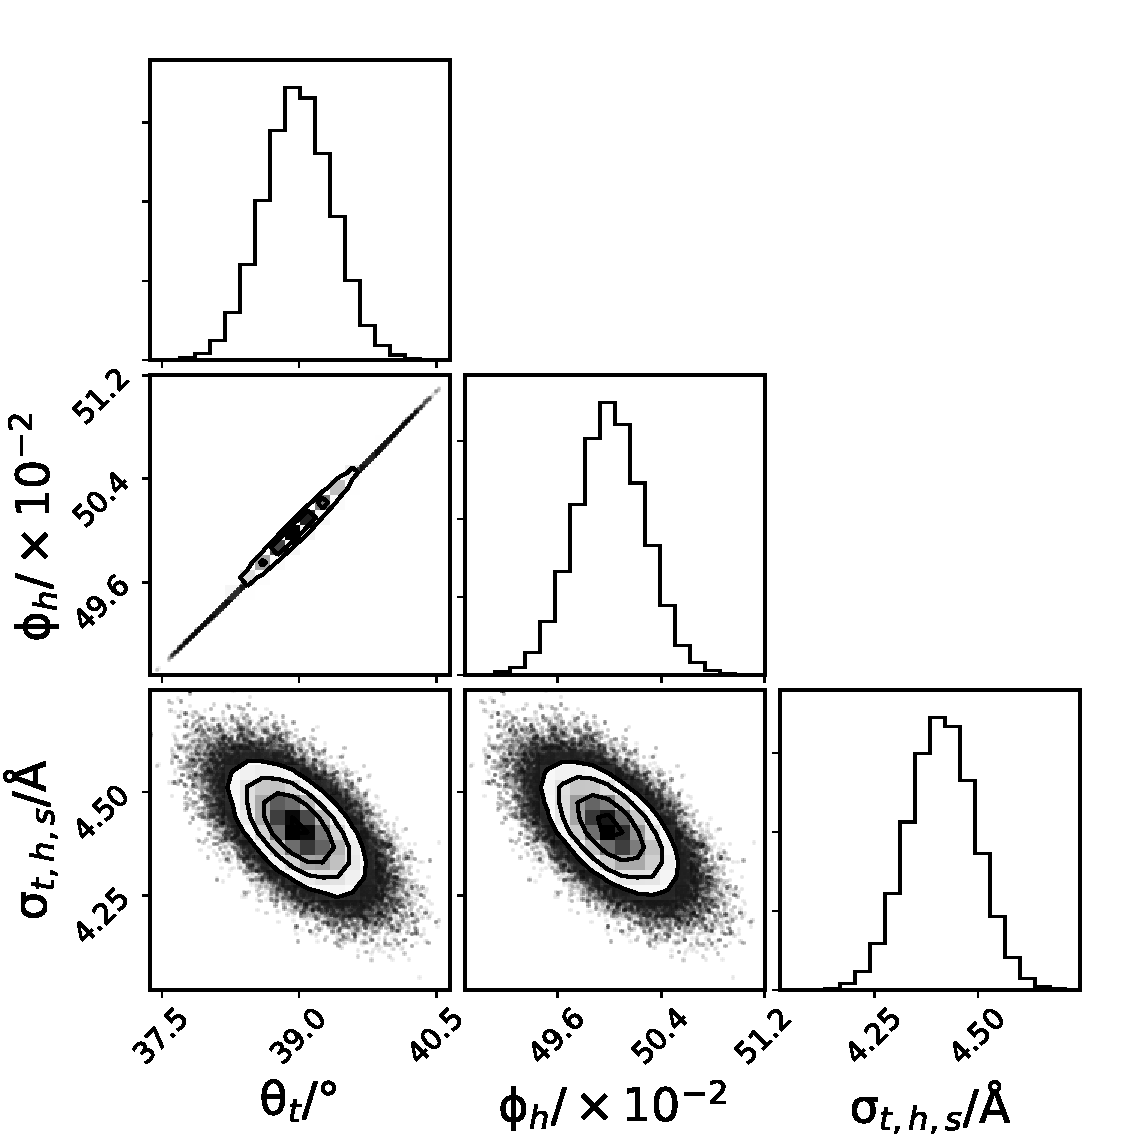
\includegraphics[width=0.50\textwidth]{figures/dmpc_20n_all_corner}
	\caption{The multi-parameter PDFs for the chemically-relevant model of two contrast DMPC neutron reflectometry data at 20 mNm$^{-1}$. Source: Datasets, figure files and running/plotting scripts are available under CC-BY.\cite{mccluskey_2018}}
	\label{fig:dmpcn1}
\end{figure}
\begin{figure}[h]
	\centering
	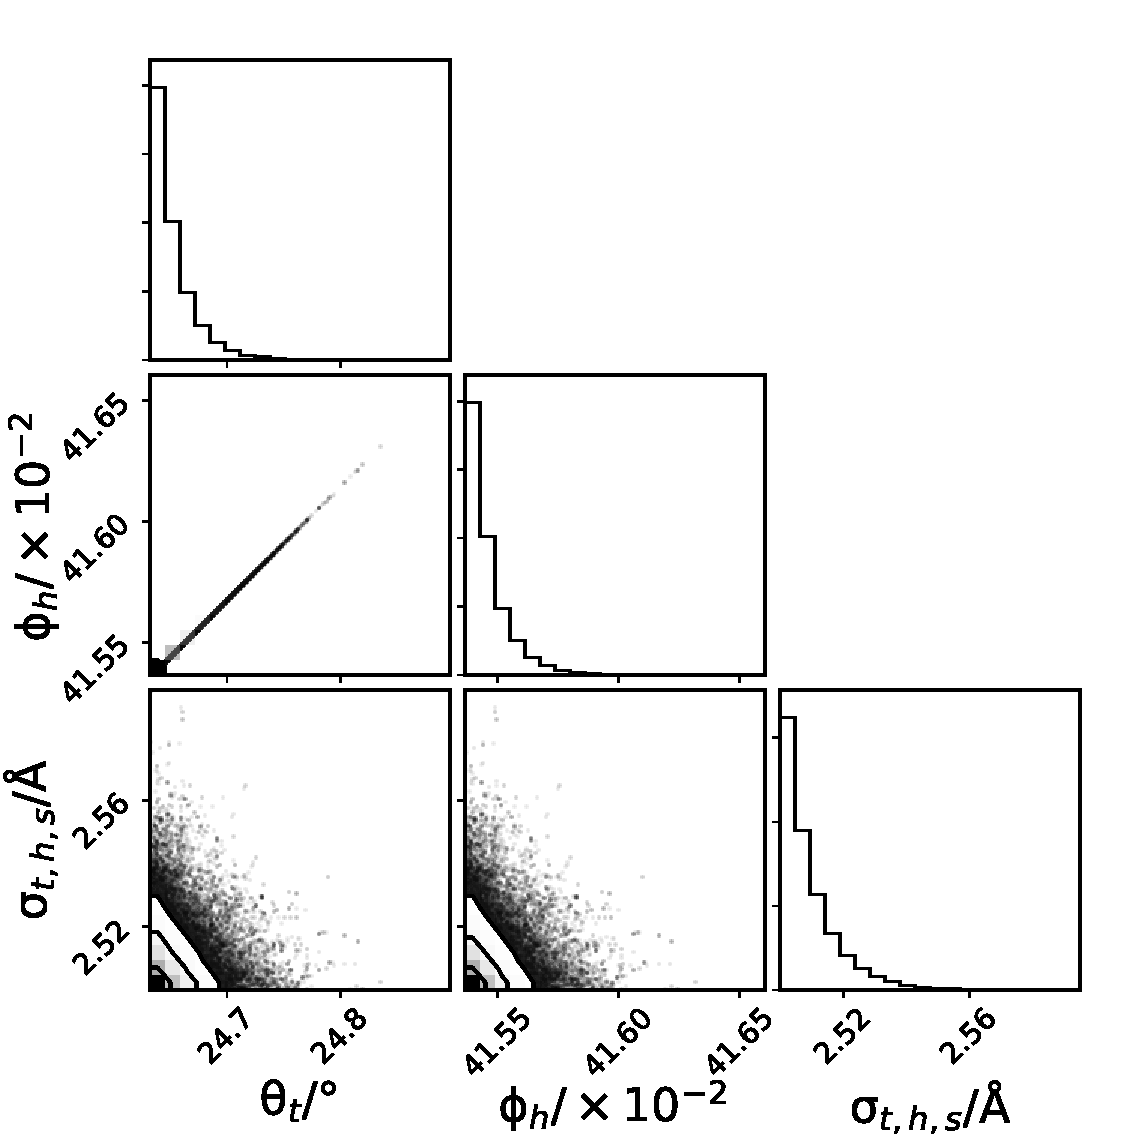
\includegraphics[width=0.50\textwidth]{figures/dmpc_25n_all_corner}
	\caption{The multi-parameter PDFs for the chemically-relevant model of two contrast DMPC neutron reflectometry data at 25 mNm$^{-1}$. Source: Datasets, figure files and running/plotting scripts are available under CC-BY.\cite{mccluskey_2018}}
	\label{fig:dmpcn2}
\end{figure}
\begin{figure}[h]
	\centering
	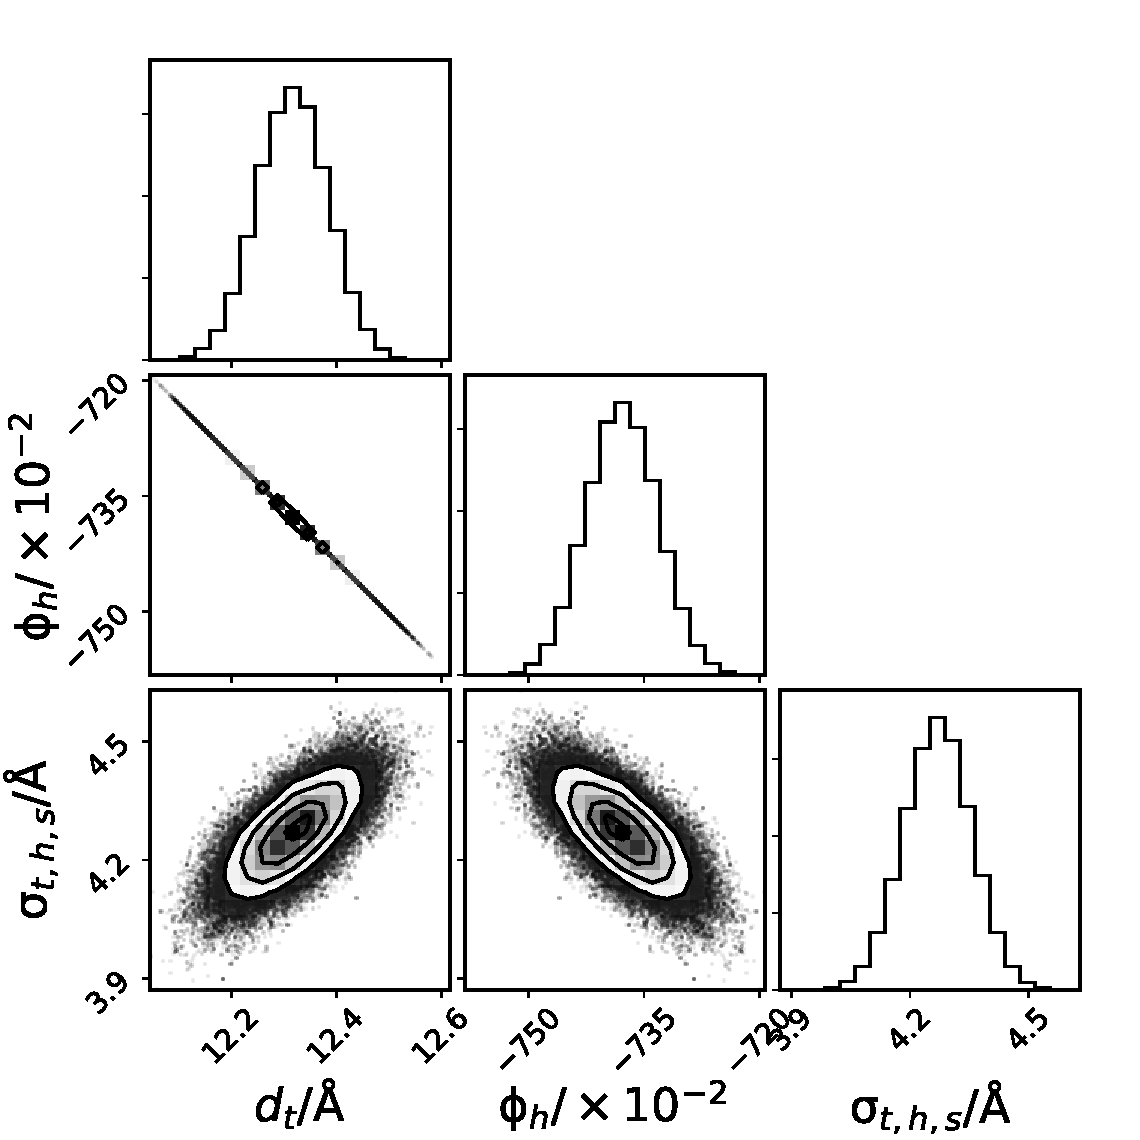
\includegraphics[width=0.50\textwidth]{figures/dppc_15n_all_corner}
	\caption{The multi-parameter PDFs for the chemically-relevant model of two contrast DPPC neutron reflectometry data at 15 mNm$^{-1}$. Source: Datasets, figure files and running/plotting scripts are available under CC-BY.\cite{mccluskey_2018}}
	\label{fig:dppcn1}
\end{figure}
\begin{figure}[h]
	\centering
	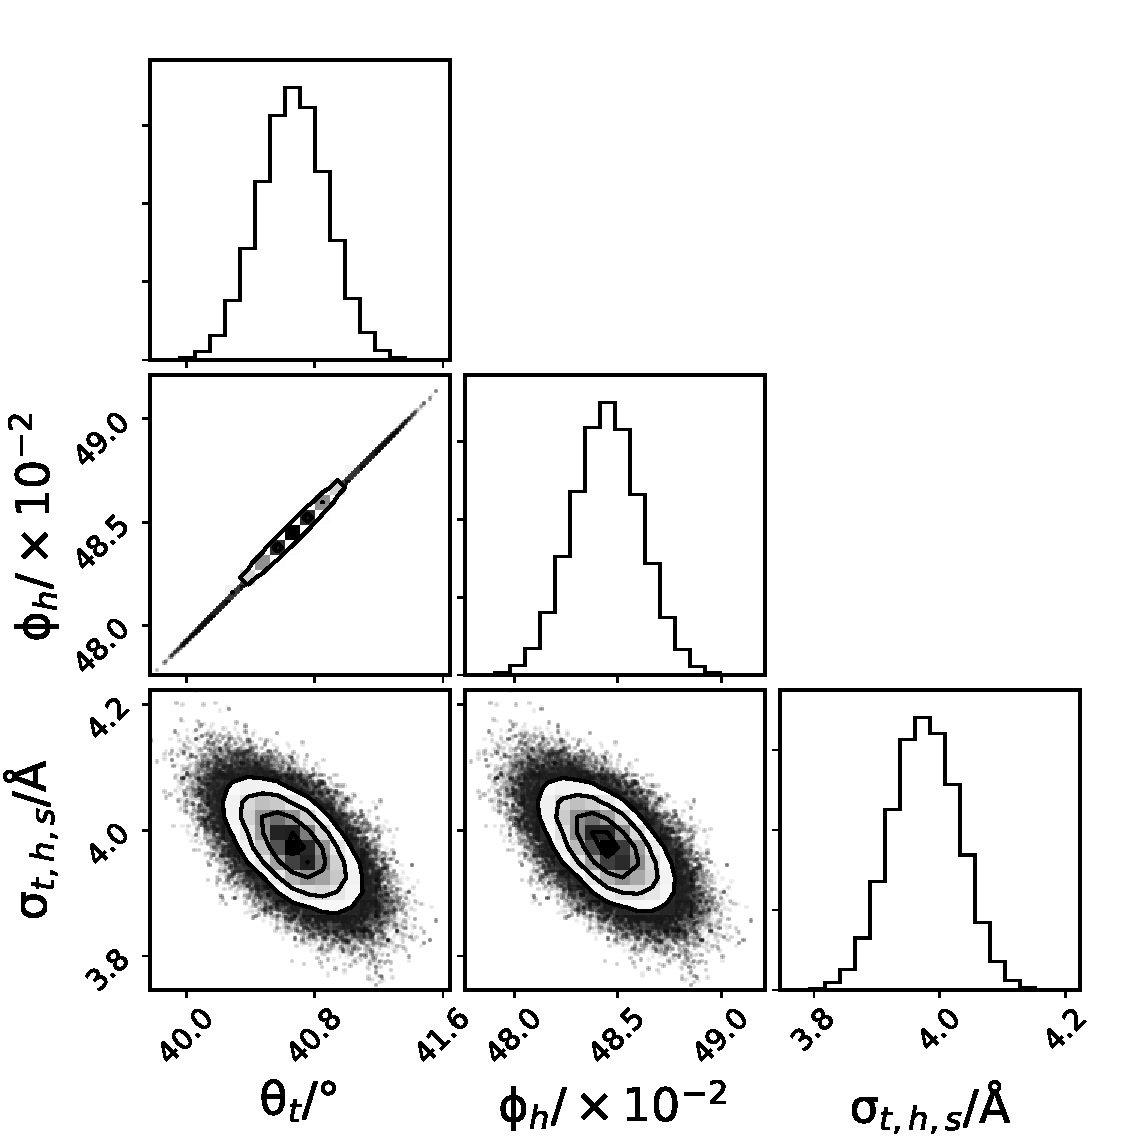
\includegraphics[width=0.50\textwidth]{figures/dppc_20n_all_corner}
	\caption{The multi-parameter PDFs for the chemically-relevant model of two contrast DMPC neutron reflectometry data at 20 mNm$^{-1}$. Source: Datasets, figure files and running/plotting scripts are available under CC-BY.\cite{mccluskey_2018}}
	\label{fig:dppcn2}
\end{figure}

%%%REFERENCES%%%
\bibliography{rsc} %You need to replace "rsc" on this line with the name of your .bib file
\bibliographystyle{rsc} %the RSC's .bst file
\end{document}
